%%%%%%%%%%%%%%%%%%%%%%%%%%%%%%%%%%%%%%%%%
% The Legrand Orange Book
% LaTeX Template
% Version 2.1.1 (14/2/16)
%
% This template has been downloaded from:
% http://www.LaTeXTemplates.com
%
% Original author:
% Mathias Legrand (legrand.mathias@gmail.com) with modifications by:
% Vel (vel@latextemplates.com)
%
% License:
% CC BY-NC-SA 3.0 (http://creativecommons.org/licenses/by-nc-sa/3.0/)
%
% Compiling this template:
% This template uses biber for its bibliography and makeindex for its index.
% When you first open the template, compile it from the command line with the
% commands below to make sure your LaTeX distribution is configured correctly:
%
% 1) pdflatex main
% 2) makeindex main.idx -s StyleInd.ist
% 3) biber main
% 4) pdflatex main x 2
%
% After this, when you wish to update the bibliography/index use the appropriate
% command above and make sure to compile with pdflatex several times
% afterwards to propagate your changes to the document.
%
% This template also uses a number of packages which may need to be
% updated to the newest versions for the template to compile. It is strongly
% recommended you update your LaTeX distribution if you have any
% compilation errors.
%
% Important note:
% Chapter heading images should have a 2:1 width:height ratio,
% e.g. 920px width and 460px height.
%
%%%%%%%%%%%%%%%%%%%%%%%%%%%%%%%%%%%%%%%%%

%----------------------------------------------------------------------------------------
%	PACKAGES AND OTHER DOCUMENT CONFIGURATIONS
%----------------------------------------------------------------------------------------

\documentclass[11pt,fleqn]{book} % Default font size and left-justified equations

%----------------------------------------------------------------------------------------

%%%%%%%%%%%%%%%%%%%%%%%%%%%%%%%%%%%%%%%%%
% The Legrand Orange Book
% Structural Definitions File
% Version 2.0 (9/2/15)
%
% Original author:
% Mathias Legrand (legrand.mathias@gmail.com) with modifications by:
% Vel (vel@latextemplates.com)
%
% This file has been downloaded from:
% http://www.LaTeXTemplates.com
%
% License:
% CC BY-NC-SA 3.0 (http://creativecommons.org/licenses/by-nc-sa/3.0/)
%
%%%%%%%%%%%%%%%%%%%%%%%%%%%%%%%%%%%%%%%%%

%----------------------------------------------------------------------------------------
%	VARIOUS REQUIRED PACKAGES AND CONFIGURATIONS
%----------------------------------------------------------------------------------------

\usepackage[top=25mm,bottom=17mm,left=20mm,right=15mm,headsep=10pt,a4paper]{geometry} % Page margins

\usepackage{wrapfig}
\usepackage{graphicx} % Required for including pictures
\graphicspath{{images/}} % Specifies the directory where pictures are stored

\usepackage{lipsum} % Inserts dummy text

\usepackage{tikz} % Required for drawing custom shapes

\usepackage[ngerman]{babel} % German language/hyphenation

\usepackage{enumitem} % Customize lists
\setlist{nolistsep} % Reduce spacing between bullet points and numbered lists

\usepackage{booktabs} % Required for nicer horizontal rules in tables

\usepackage{xcolor} % Required for specifying colors by name
\definecolor{hhublue}{RGB}{0,106,179} % Define the orange color used for highlighting throughout the book

\usepackage{sectsty}
\usepackage{algpseudocode}
%\usepackage{algorithm}
\usepackage{algorithm2e}
\usepackage{listingsutf8}
\usepackage{pgf}
\usepackage{float}
\usetikzlibrary{arrows, calc}

\lstset{float,frame=single,basicstyle=\small\ttfamily,numbers=left,firstnumber=1}


%----------------------------------------------------------------------------------------
%	FONTS
%----------------------------------------------------------------------------------------

\usepackage{avant} % Use the Avantgarde font for headings
%\usepackage{times} % Use the Times font for headings
\usepackage{mathptmx} % Use the Adobe Times Roman as the default text font together with math symbols from the Sym­bol, Chancery and Com­puter Modern fonts

\usepackage{microtype} % Slightly tweak font spacing for aesthetics
\usepackage[utf8]{inputenc} % Required for including letters with accents
\usepackage[T1]{fontenc} % Use 8-bit encoding that has 256 glyphs
\usepackage{csquotes}

%----------------------------------------------------------------------------------------
%	BIBLIOGRAPHY AND INDEX
%----------------------------------------------------------------------------------------

\usepackage[style=alphabetic,citestyle=alphabetic,sorting=nyt,sortcites=true,autopunct=true,babel=hyphen,hyperref=true,abbreviate=false,backref=true,backend=biber]{biblatex}
\addbibresource{bibliography.bib} % BibTeX bibliography file
\defbibheading{bibempty}{}

\usepackage{calc} % For simpler calculation - used for spacing the index letter headings correctly
\usepackage{makeidx} % Required to make an index
\makeindex % Tells LaTeX to create the files required for indexing

%----------------------------------------------------------------------------------------
%	MAIN TABLE OF CONTENTS
%----------------------------------------------------------------------------------------

\usepackage{titletoc} % Required for manipulating the table of contents

\contentsmargin{0cm} % Removes the default margin

% Part text styling
\titlecontents{part}[0cm]
{\addvspace{20pt}\centering\large\bfseries}
{}
{}
{}

% Chapter text styling
\titlecontents{chapter}[1.25cm] % Indentation
{\addvspace{12pt}\large\sffamily\bfseries} % Spacing and font options for chapters
{\color{hhublue!70}\contentslabel[\Large\thecontentslabel]{1.25cm}\color{hhublue}} % Chapter number
{\color{hhublue}}
{\color{hhublue!70}\normalsize\;\titlerule*[.5pc]{.}\;\thecontentspage} % Page number

% Section text styling
\titlecontents{section}[1.25cm] % Indentation
{\addvspace{3pt}\sffamily\bfseries} % Spacing and font options for sections
{\contentslabel[\thecontentslabel]{1.25cm}} % Section number
{}
{\hfill\color{black}\thecontentspage} % Page number
[]

% Subsection text styling
\titlecontents{subsection}[1.25cm] % Indentation
{\addvspace{1pt}\sffamily\small} % Spacing and font options for subsections
{\contentslabel[\thecontentslabel]{1.25cm}} % Subsection number
{}
{\ \titlerule*[.5pc]{.}\;\thecontentspage} % Page number
[]

% List of figures
\titlecontents{figure}[0em]
{\addvspace{-5pt}\sffamily}
{\thecontentslabel\hspace*{1em}}
{}
{\ \titlerule*[.5pc]{.}\;\thecontentspage}
[]

% List of tables
\titlecontents{table}[0em]
{\addvspace{-5pt}\sffamily}
{\thecontentslabel\hspace*{1em}}
{}
{\ \titlerule*[.5pc]{.}\;\thecontentspage}
[]

%----------------------------------------------------------------------------------------
%	MINI TABLE OF CONTENTS IN PART HEADS
%----------------------------------------------------------------------------------------

% Chapter text styling
\titlecontents{lchapter}[0em] % Indenting
{\addvspace{15pt}\large\sffamily\bfseries} % Spacing and font options for chapters
{\color{hhublue}\contentslabel[\Large\thecontentslabel]{1.25cm}\color{hhublue}} % Chapter number
{}
{\color{hhublue}\normalsize\sffamily\bfseries\;\titlerule*[.5pc]{.}\;\thecontentspage} % Page number

% Section text styling
\titlecontents{lsection}[0em] % Indenting
{\sffamily\small} % Spacing and font options for sections
{\contentslabel[\thecontentslabel]{1.25cm}} % Section number
{}
{}

% Subsection text styling
\titlecontents{lsubsection}[.5em] % Indentation
{\normalfont\footnotesize\sffamily} % Font settings
{}
{}
{}

%----------------------------------------------------------------------------------------
%	PAGE HEADERS
%----------------------------------------------------------------------------------------

\usepackage{fancyhdr} % Required for header and footer configuration

\pagestyle{fancy}
\renewcommand{\chaptermark}[1]{\markboth{\sffamily\normalsize\bfseries\chaptername\ \thechapter.\ #1}{}} % Chapter text font settings
\renewcommand{\sectionmark}[1]{\markright{\sffamily\normalsize\thesection\hspace{5pt}#1}{}} % Section text font settings
\fancyhf{} \fancyhead[LE,RO]{\sffamily\normalsize\thepage} % Font setting for the page number in the header
\fancyhead[LO]{\rightmark} % Print the nearest section name on the left side of odd pages
\fancyhead[RE]{\leftmark} % Print the current chapter name on the right side of even pages
\renewcommand{\headrulewidth}{0.5pt} % Width of the rule under the header
\addtolength{\headheight}{2.5pt} % Increase the spacing around the header slightly
\renewcommand{\footrulewidth}{0pt} % Removes the rule in the footer
\fancypagestyle{plain}{\fancyhead{}\renewcommand{\headrulewidth}{0pt}} % Style for when a plain pagestyle is specified

% Removes the header from odd empty pages at the end of chapters
\makeatletter
\renewcommand{\cleardoublepage}{
\clearpage\ifodd\c@page\else
\hbox{}
\vspace*{\fill}
\thispagestyle{empty}
\newpage
\fi}

%----------------------------------------------------------------------------------------
%	THEOREM STYLES
%----------------------------------------------------------------------------------------

\usepackage{amsmath,amsfonts,amssymb,amsthm} % For math equations, theorems, symbols, etc

\newcommand{\intoo}[2]{\mathopen{]}#1\,;#2\mathclose{[}}
\newcommand{\ud}{\mathop{\mathrm{{}d}}\mathopen{}}
\newcommand{\intff}[2]{\mathopen{[}#1\,;#2\mathclose{]}}
\newtheorem{notation}{Notation}[chapter]

% Boxed/framed environments
\newtheoremstyle{hhubluenumbox}% % Theorem style name
{0pt}% Space above
{0pt}% Space below
{\normalfont}% % Body font
{}% Indent amount
{\small\bf\sffamily\color{hhublue}}% % Theorem head font
{\;}% Punctuation after theorem head
{0.25em}% Space after theorem head
{\small\sffamily\color{hhublue}\thmname{#1}\nobreakspace\thmnumber{\@ifnotempty{#1}{}\@upn{#2}}% Theorem text (e.g. Theorem 2.1)
\thmnote{\nobreakspace\the\thm@notefont\sffamily\bfseries\color{black}---\nobreakspace#3.}} % Optional theorem note
\renewcommand{\qedsymbol}{$\blacksquare$}% Optional qed square

\newtheoremstyle{blacknumex}% Theorem style name
{5pt}% Space above
{5pt}% Space below
{\normalfont}% Body font
{} % Indent amount
{\small\bf\sffamily}% Theorem head font
{\;}% Punctuation after theorem head
{0.25em}% Space after theorem head
{\small\sffamily{\tiny\ensuremath{\blacksquare}}\nobreakspace\thmname{#1}\nobreakspace\thmnumber{\@ifnotempty{#1}{}\@upn{#2}}% Theorem text (e.g. Theorem 2.1)
\thmnote{\nobreakspace\the\thm@notefont\sffamily\bfseries---\nobreakspace#3.}}% Optional theorem note

\newtheoremstyle{blacknumbox} % Theorem style name
{0pt}% Space above
{0pt}% Space below
{\normalfont}% Body font
{}% Indent amount
{\small\bf\sffamily}% Theorem head font
{\;}% Punctuation after theorem head
{0.25em}% Space after theorem head
{\small\sffamily\thmname{#1}\nobreakspace\thmnumber{\@ifnotempty{#1}{}\@upn{#2}}% Theorem text (e.g. Theorem 2.1)
\thmnote{\nobreakspace\the\thm@notefont\sffamily\bfseries---\nobreakspace#3.}}% Optional theorem note

% Non-boxed/non-framed environments
\newtheoremstyle{hhubluenum}% % Theorem style name
{5pt}% Space above
{5pt}% Space below
{\normalfont}% % Body font
{}% Indent amount
{\small\bf\sffamily\color{hhublue}}% % Theorem head font
{\;}% Punctuation after theorem head
{0.25em}% Space after theorem head
{\small\sffamily\color{hhublue}\thmname{#1}\nobreakspace\thmnumber{\@ifnotempty{#1}{}\@upn{#2}}% Theorem text (e.g. Theorem 2.1)
\thmnote{\nobreakspace\the\thm@notefont\sffamily\bfseries\color{black}---\nobreakspace#3.}} % Optional theorem note
\renewcommand{\qedsymbol}{$\blacksquare$}% Optional qed square
\makeatother

% Defines the theorem text style for each type of theorem to one of the three styles above
\newcounter{dummy}
\numberwithin{dummy}{section}
\theoremstyle{hhubluenumbox}
\newtheorem{theoremeT}[dummy]{Theorem}
\newtheorem{problem}{Problem}[chapter]
\newtheorem{exerciseT}{Exercise}[chapter]
\theoremstyle{blacknumex}
\newtheorem{exampleT}{Example}[chapter]
\theoremstyle{blacknumbox}
\newtheorem{vocabulary}{Vocabulary}[chapter]
\newtheorem{definitionT}{Definition}[section]
\newtheorem{corollaryT}[dummy]{Corollary}
\theoremstyle{hhubluenum}
\newtheorem{proposition}[dummy]{Proposition}

%----------------------------------------------------------------------------------------
%	DEFINITION OF COLORED BOXES
%----------------------------------------------------------------------------------------

\RequirePackage[framemethod=default]{mdframed} % Required for creating the theorem, definition, exercise and corollary boxes

% Theorem box
\newmdenv[skipabove=7pt,
skipbelow=7pt,
backgroundcolor=black!5,
linecolor=hhublue,
innerleftmargin=5pt,
innerrightmargin=5pt,
innertopmargin=5pt,
leftmargin=0cm,
rightmargin=0cm,
innerbottommargin=5pt]{tBox}

% Exercise box
\newmdenv[skipabove=7pt,
skipbelow=7pt,
rightline=false,
leftline=true,
topline=false,
bottomline=false,
backgroundcolor=hhublue!10,
linecolor=hhublue,
innerleftmargin=5pt,
innerrightmargin=5pt,
innertopmargin=5pt,
innerbottommargin=5pt,
leftmargin=0cm,
rightmargin=0cm,
linewidth=4pt]{eBox}

% Definition box
\newmdenv[skipabove=7pt,
skipbelow=7pt,
rightline=false,
leftline=true,
topline=false,
bottomline=false,
linecolor=hhublue,
innerleftmargin=5pt,
innerrightmargin=5pt,
innertopmargin=0pt,
leftmargin=0cm,
rightmargin=0cm,
linewidth=4pt,
innerbottommargin=0pt]{dBox}

% Corollary box
\newmdenv[skipabove=7pt,
skipbelow=7pt,
rightline=false,
leftline=true,
topline=false,
bottomline=false,
linecolor=gray,
backgroundcolor=black!5,
innerleftmargin=5pt,
innerrightmargin=5pt,
innertopmargin=5pt,
leftmargin=0cm,
rightmargin=0cm,
linewidth=4pt,
innerbottommargin=5pt]{cBox}

% Creates an environment for each type of theorem and assigns it a theorem text style from the "Theorem Styles" section above and a colored box from above
\newenvironment{theorem}{\begin{tBox}\begin{theoremeT}}{\end{theoremeT}\end{tBox}}
\newenvironment{exercise}{\begin{eBox}\begin{exerciseT}}{\hfill{\color{hhublue}\tiny\ensuremath{\blacksquare}}\end{exerciseT}\end{eBox}}
\newenvironment{definition}{\begin{dBox}\begin{definitionT}}{\end{definitionT}\end{dBox}}
\newenvironment{example}{\begin{exampleT}}{\hfill{\tiny\ensuremath{\blacksquare}}\end{exampleT}}
\newenvironment{corollary}{\begin{cBox}\begin{corollaryT}}{\end{corollaryT}\end{cBox}}

%----------------------------------------------------------------------------------------
%	REMARK ENVIRONMENT
%----------------------------------------------------------------------------------------

\newenvironment{remark}{\par\vspace{10pt}\small % Vertical white space above the remark and smaller font size
\begin{list}{}{
\leftmargin=35pt % Indentation on the left
\rightmargin=25pt}\item\ignorespaces % Indentation on the right
\makebox[-2.5pt]{\begin{tikzpicture}[overlay]
\node[draw=hhublue!70,line width=1pt,circle,fill=hhublue!25,font=\sffamily\bfseries,inner sep=2pt,outer sep=0pt] at (-15pt,0pt){\textcolor{hhublue}{R}};\end{tikzpicture}} % Orange R in a circle
\advance\baselineskip -1pt}{\end{list}\vskip5pt} % Tighter line spacing and white space after remark

%----------------------------------------------------------------------------------------
%	SECTION NUMBERING IN THE MARGIN
%----------------------------------------------------------------------------------------

\makeatletter
\renewcommand{\@seccntformat}[1]{\llap{\textcolor{hhublue}{\csname the#1\endcsname}\hspace{1em}}}
\renewcommand{\section}{\@startsection{section}{1}{\z@}
{-4ex \@plus -1ex \@minus -.4ex}
{1ex \@plus.2ex }
{\normalfont\large\sffamily\bfseries}}
\renewcommand{\subsection}{\@startsection {subsection}{2}{\z@}
{-3ex \@plus -0.1ex \@minus -.4ex}
{0.5ex \@plus.2ex }
{\normalfont\sffamily\bfseries}}
\renewcommand{\subsubsection}{\@startsection {subsubsection}{3}{\z@}
{-2ex \@plus -0.1ex \@minus -.2ex}
{.2ex \@plus.2ex }
{\normalfont\small\sffamily\bfseries}}
\renewcommand\paragraph{\@startsection{paragraph}{4}{\z@}
{-2ex \@plus-.2ex \@minus .2ex}
{.1ex}
{\normalfont\small\sffamily\bfseries}}

%----------------------------------------------------------------------------------------
%	PART HEADINGS
%----------------------------------------------------------------------------------------

% numbered part in the table of contents
\newcommand{\@mypartnumtocformat}[2]{%
\setlength\fboxsep{0pt}%
\noindent\colorbox{hhublue!30}{\strut\parbox[c][.7cm]{\ecart}{\color{hhublue!70}\Large\sffamily\bfseries\centering#1}}\hskip\esp\colorbox{hhublue!50}{\strut\parbox[c][.7cm]{\linewidth-\ecart-\esp}{\Large\sffamily\centering#2}}}%
%%%%%%%%%%%%%%%%%%%%%%%%%%%%%%%%%%
% unnumbered part in the table of contents
\newcommand{\@myparttocformat}[1]{%
\setlength\fboxsep{0pt}%
\noindent\colorbox{hhublue!50}{\strut\parbox[c][.7cm]{\linewidth}{\Large\sffamily\centering#1}}}%
%%%%%%%%%%%%%%%%%%%%%%%%%%%%%%%%%%
\newlength\esp
\setlength\esp{4pt}
\newlength\ecart
\setlength\ecart{1.2cm-\esp}
\newcommand{\thepartimage}{}%
\newcommand{\partimage}[1]{\renewcommand{\thepartimage}{#1}}%
\def\@part[#1]#2{%
\ifnum \c@secnumdepth >-2\relax%
\refstepcounter{part}%
\addcontentsline{toc}{part}{\texorpdfstring{\protect\@mypartnumtocformat{\thepart}{#1}}{\partname~\thepart\ ---\ #1}}
\else%
\addcontentsline{toc}{part}{\texorpdfstring{\protect\@myparttocformat{#1}}{#1}}%
\fi%
\startcontents%
\markboth{}{}%
{\thispagestyle{empty}%
\begin{tikzpicture}[remember picture,overlay]%
\node at (current page.north west){\begin{tikzpicture}[remember picture,overlay]%
\fill[hhublue!30](0cm,0cm) rectangle (\paperwidth,-\paperheight);
\node[anchor=north] at (4cm,-3.25cm){\color{hhublue!50}\fontsize{220}{100}\sffamily\bfseries\@Roman\c@part};
\node[anchor=south east] at (\paperwidth-1cm,-\paperheight+1cm){\parbox[t][][t]{8.5cm}{
\printcontents{l}{0}{\setcounter{tocdepth}{1}}%
}};
\node[anchor=north east] at (\paperwidth-1.5cm,-3.25cm){\parbox[t][][t]{15cm}{\strut\raggedleft\color{white}\fontsize{30}{30}\sffamily\bfseries#2}};
\end{tikzpicture}};
\end{tikzpicture}}%
\@endpart}
\def\@spart#1{%
\startcontents%
\phantomsection
{\thispagestyle{empty}%
\begin{tikzpicture}[remember picture,overlay]%
\node at (current page.north west){\begin{tikzpicture}[remember picture,overlay]%
\fill[hhublue!30](0cm,0cm) rectangle (\paperwidth,-\paperheight);
\node[anchor=north east] at (\paperwidth-1.5cm,-3.25cm){\parbox[t][][t]{15cm}{\strut\raggedleft\color{white}\fontsize{30}{30}\sffamily\bfseries#1}};
\end{tikzpicture}};
\end{tikzpicture}}
\addcontentsline{toc}{part}{\texorpdfstring{%
\setlength\fboxsep{0pt}%
\noindent\protect\colorbox{hhublue!50}{\strut\protect\parbox[c][.7cm]{\linewidth}{\Large\sffamily\protect\centering #1\quad\mbox{}}}}{#1}}%
\@endpart}
\def\@endpart{\vfil\newpage
\if@twoside
\if@openright
\null
\thispagestyle{empty}%
\newpage
\fi
\fi
\if@tempswa
\twocolumn
\fi}

%----------------------------------------------------------------------------------------
%	CHAPTER HEADINGS
%----------------------------------------------------------------------------------------

% A switch to conditionally include a picture, implemented by  Christian Hupfer
\newif\ifusechapterimage
\usechapterimagetrue
\newcommand{\thechapterimage}{}%
\newcommand{\chapterimage}[1]{\ifusechapterimage\renewcommand{\thechapterimage}{#1}\fi}%
\def\@makechapterhead#1{%
{\parindent \z@ \raggedright \normalfont
\ifnum \c@secnumdepth >\m@ne
\if@mainmatter
\begin{tikzpicture}[remember picture,overlay]
\node at (current page.north west)
{\begin{tikzpicture}[remember picture,overlay]
\node[anchor=north west,inner sep=0pt] at (0,0) {\ifusechapterimage\includegraphics[width=\paperwidth]{\thechapterimage}\fi};
\draw[anchor=west] (\Gm@lmargin,-9cm) node [line width=2pt,rounded corners=15pt,draw=hhublue,fill=white,fill opacity=0.5,inner sep=15pt]{\strut\makebox[22cm]{}};
\draw[anchor=west] (\Gm@lmargin+.3cm,-9cm) node {\huge\sffamily\bfseries\color{black}\thechapter. #1\strut};
\end{tikzpicture}};
\end{tikzpicture}
\else
\begin{tikzpicture}[remember picture,overlay]
\node at (current page.north west)
{\begin{tikzpicture}[remember picture,overlay]
\node[anchor=north west,inner sep=0pt] at (0,0) {\ifusechapterimage\includegraphics[width=\paperwidth]{\thechapterimage}\fi};
\draw[anchor=west] (\Gm@lmargin,-9cm) node [line width=2pt,rounded corners=15pt,draw=hhublue,fill=white,fill opacity=0.5,inner sep=15pt]{\strut\makebox[22cm]{}};
\draw[anchor=west] (\Gm@lmargin+.3cm,-9cm) node {\huge\sffamily\bfseries\color{black}#1\strut};
\end{tikzpicture}};
\end{tikzpicture}
\fi\fi\par\vspace*{270\p@}}}

%-------------------------------------------

\def\@makeschapterhead#1{%
\begin{tikzpicture}[remember picture,overlay]
\node at (current page.north west)
{\begin{tikzpicture}[remember picture,overlay]
\node[anchor=north west,inner sep=0pt] at (0,0) {\ifusechapterimage\includegraphics[width=\paperwidth]{\thechapterimage}\fi};
\draw[anchor=west] (\Gm@lmargin,-9cm) node [line width=2pt,rounded corners=15pt,draw=hhublue,fill=white,fill opacity=0.5,inner sep=15pt]{\strut\makebox[22cm]{}};
\draw[anchor=west] (\Gm@lmargin+.3cm,-9cm) node {\huge\sffamily\bfseries\color{black}#1\strut};
\end{tikzpicture}};
\end{tikzpicture}
\par\vspace*{270\p@}}
\makeatother

%----------------------------------------------------------------------------------------
%	HYPERLINKS IN THE DOCUMENTS
%----------------------------------------------------------------------------------------

\usepackage{hyperref}
\hypersetup{hidelinks,backref=true,pagebackref=true,hyperindex=true,colorlinks=false,breaklinks=true,urlcolor= hhublue,bookmarks=true,bookmarksopen=false,pdftitle={Title},pdfauthor={Author}}
\usepackage{bookmark}
\bookmarksetup{
open,
numbered,
addtohook={%
\ifnum\bookmarkget{level}=0 % chapter
\bookmarksetup{bold}%
\fi
\ifnum\bookmarkget{level}=-1 % part
\bookmarksetup{color=hhublue,bold}%
\fi
}
}
 % Insert the commands.tex file which contains the majority of the structure behind the template

\begin{document}

%----------------------------------------------------------------------------------------
%	TITLE PAGE
%----------------------------------------------------------------------------------------

\begingroup
\thispagestyle{empty}
\begin{tikzpicture}[remember picture,overlay]
\coordinate [below=12cm] (midpoint) at (current page.north);
\node at (current page.north west)
{\begin{tikzpicture}[remember picture,overlay]
\node[anchor=north west,inner sep=0pt] at (0,0) {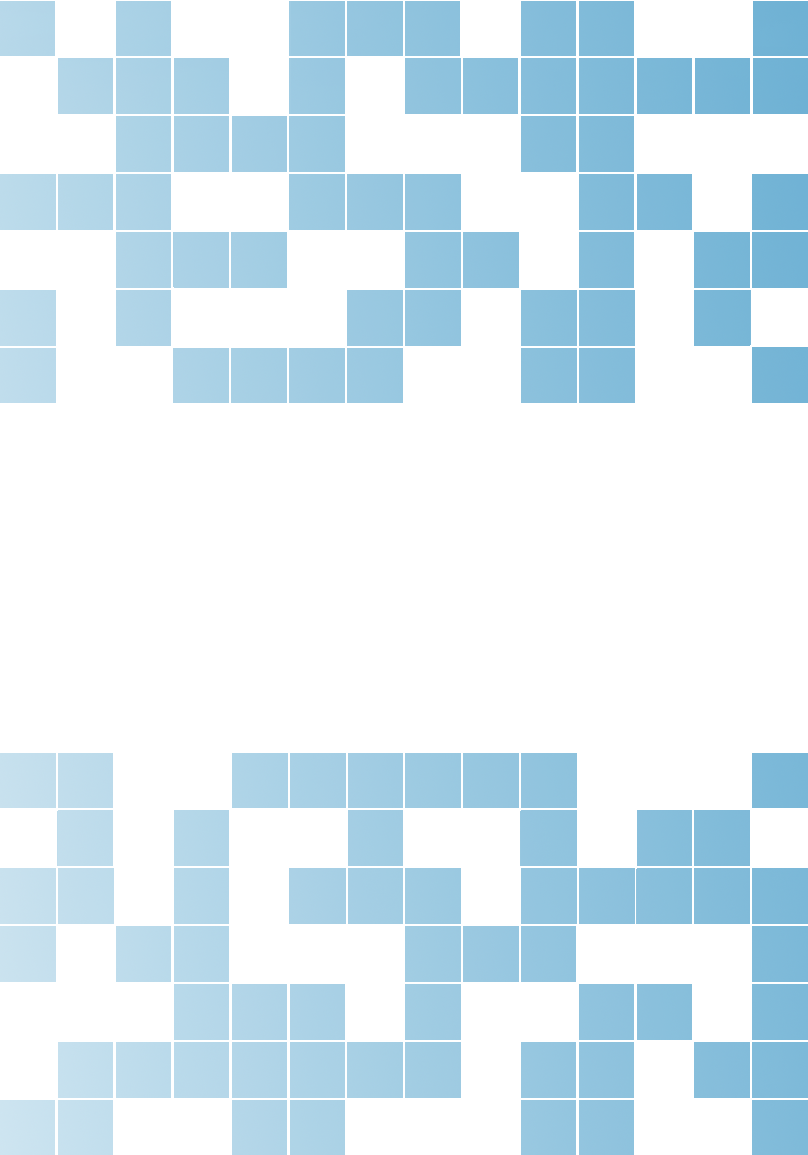
\includegraphics[width=\paperwidth]{background}}; % Background image
\draw[anchor=north] (midpoint) node [fill=hhublue!30!white,fill opacity=0.6,text opacity=1,inner sep=1cm]{\Huge\centering\bfseries\sffamily\parbox[c][][t]{\paperwidth}{\centering Grundlagen der künstlichen Intelligenz\\[15pt] % Book title
{\Large Vorlesungsskript zum Seminar im SS 2016}\\[20pt] % Subtitle
{\huge Michael Leuschel \& Sebastian Krings}}}; % Author name
\end{tikzpicture}};
\end{tikzpicture}
\vfill
\endgroup

%----------------------------------------------------------------------------------------
%	COPYRIGHT PAGE
%----------------------------------------------------------------------------------------

\newpage
~\vfill
\thispagestyle{empty}

\noindent Copyright \copyright\ 2016 Michael Leuschel, Sebastian Krings and others\\ % Copyright notice

%\noindent \textsc{Published by Publisher}\\ % Publisher

\noindent \url{http://www.stups.hhu.de}\\ % URL

\noindent
\begin{wrapfigure}[4]{l}[0cm]{0.0\textwidth}
%  \begin{center}

\includegraphics{images/creativecommons.png}
 % \end{center}
\end{wrapfigure}
 Licensed under the Creative Commons Attribution-NonCommercial-NoDerivatives 4.0 International Public License (the ``License''). You may not use this file except in compliance with the License. You may obtain a copy of the License at \url{http://creativecommons.org/licenses/by-nc-nd/4.0/}. Unless required by applicable law or agreed to in writing, software distributed under the License is distributed on an \textsc{``as is'' basis, without warranties or conditions of any kind}, either express or implied. See the License for the specific language governing permissions and limitations under the License.\\ % License information

%\noindent \textit{First printing, March 2013} % Printing/edition date

%----------------------------------------------------------------------------------------
%	COPYRIGHT AND THANKS PAGE
%----------------------------------------------------------------------------------------

\newpage
%~\vfill
\thispagestyle{empty}

\noindent This book and the corresponding slides are based on work of the students of our artifical intelligence course. We would like to thank all contributors.

\noindent
The contributors are (in alphabetical order):
\begin{itemize}
    \item Batiukova, Olga
    \item Brenneis, Markus
    \item Brümmer, Ronny
    \item Happe, Chistopher
    \item Kerkmann, Anna Maria
    \item Krzysztala, Denis
    \item Moreira Hamasaki, Thaís
    \item Nalecz, Rafael
    \item Oberländer, Nils
    \item Özen, Eyyüp
    \item Papenberg, Martin
    \item Petrasch, Jessica
    \item Schmidt, Joshua
    \item Sura, Sebastian
    \item Thelen, Alexander
    \item Ullrich, Julian
    \item Weck, Sandy
    \item Weißenfeld, Anke Leonie
\end{itemize}

%\noindent \textit{First printing, March 2013} % Printing/edition date

%----------------------------------------------------------------------------------------
%	TABLE OF CONTENTS
%----------------------------------------------------------------------------------------

%\usechapterimagefalse % If you don't want to include a chapter image, use this to toggle images off - it can be enabled later with \usechapterimagetrue

\chapterimage{chapter_head_1.png} % Table of contents heading image

\pagestyle{empty} % No headers

\tableofcontents % Print the table of contents itself

\cleardoublepage % Forces the first chapter to start on an odd page so it's on the right

\pagestyle{fancy} % Print headers again

\part{Einleitung}
\chapterimage{chapter_head_1.png} % Chapter heading image

\chapter{Einleitung}


\part{Reasoning}
\chapterimage{chapter_head_1.png}

\chapter{Theorembeweiser}
\section{Einleitung}
Der Eine kennt sie überhaupt nicht, der Andere womöglich noch aus der Schule, aber wirklich
jeder Student mit Mathematikkursen kennt sie - die Beweise.
In der Mathematik werden seit jeher Theorien aufgestellt, bewiesen und mitunter auch wiederlegt.
Man kann das Beweisen dieser als eine Art Kunstform ansehen.
So gibt es häufig nicht nur den einen Weg zum Ziel, sondern oftmals auch schnellere, schönere und/oder einfachere.
Allen gemein ist allerdings, dass Außenstehende damit kaum etwas anfangen können. Nichts desto trotz resultieren die Bemühungen der Mathematiker nicht zuletzt in einen sichtbaren Nutzen.
Als ein Beispiel sei hierbei das vier Farben Problem genannt. Kurz und knapp geht es um die Frage: \enquote{Ist es möglich eine Landkarte mit lediglich vier verschiedenen Farben so einzufärben, so das am Ende alle benachbarten Länder verschiedenfarbig sind?}
Die Frage entstand bereits im 19. Jahrhundert, als das Drucken von zusätzlichen Farben noch mit erhöhtem Aufwand einher ging. 1852 formulierte Francis Guthrie erstmals dazu einen Satz als Vermutung. Dieser erlangte schnell Popularität und es folgten eine Reihe von Beweisen, welche dann früher oder später wiederlegt wurden. Erstmals bewiesen wurde er 1976 von Appel und Haken, welche zu jener Zeit frisch entwickelte Methoden zum computergestützten Beweisen von Theoremen anwendeten. Dazu wurde das Problem zunächst auf die Ebene der Graphentheorie getragen und anschließend mit einer Mischung aus klassischen und computerbasierten Beweisen zu einem positiven Ergebnis gebracht. Das allgemeine Problem wurde dabei auf 1936 Fälle (später 1478) reduziert, welche der Computer dann einzeln durchprüfen konnte. Es gibt vor allem zwei Hauptkritikpunkte an Appel und Hakens Beweis:
\begin{enumerate}
\item Es wurde ein Computer benutzt, sodass nicht alles verifiziert werden kann.
\item  Gerade der Teil, der per Hand geprüft werden müsste, ist so kompliziert und
mühsam, dass ihn, soweit bekannt, niemand unabhängig geprüft hat.
\end{enumerate}
Man wird schnell bemerken, dass dies ein durchaus stark diskutiertes Thema ist. So argumentieren Kritiker, dass Beweise stets von Menschenhand nachprüfbar und nachvollziehbar sein sollten oder zweifeln gar die Korrektheit der maschinellen Beweise an. Nun, in der Tat verstecken sich häufig Fehler in Computerprogrammen, sodass die verwendeten Algorithmen mitunter inkonsistent arbeiten. 1996 bewiesen N. Robertson, D. P. Sanders, P. Seymour und R. Thomas den Vier-Farben-Satz mit der gleichen Beweisidee, reduzierten allerdings die Anzahl der Problemfälle auf 633. Mittlerweile gibt es noch weitere unabhängige Beweise dazu. Man kann zwar nicht ausschließen, dass der Mensch oder die Maschine in einem geführten Beweis Fehler gemacht haben, aber je häufiger ein Theorem unabhängig bewiesen wird, desto
unwahrscheinlicher wird es, dass all diese Beweise fehlerhaft sind. Anhand der folgenden Tabelle von Thomas C. Hales[] sieht man, dass es seit längerem Bestrebungen gibt, mathematische Aussagen mit dem Computer zu beweisen.

\begin{table}
\begin{tabular}{ccccc}
\toprule
Jahr & Theorem & Beweissystem & Formaler Beweis & Klassischer Beweis \\ \midrule
1986 & First Incompleteness & Boyer-Moore & Shankar & Gödel \\
1990 & Quadratic Reciprocity & Boyer-Moore & Russinoff & Eisenstein \\
1996 & Fundamental - of Calculus & HOL Light & Harrison & Henstock \\
2000 & Fundamental - of Algebra & Mizar & Milewski & Brynski \\
2000 & Fundamental - of Algebra & Coq & Geuvers et al. & Kneser \\
2004 & Four-Color & Coq & Gonthier & Robertson et al. \\
2004 & Prime Number & Isabelle & Avigad et al. & Selberg-Erdös \\
2005 & Jordan Curve & HOL Light & Hales & Thomassen \\
2005 & Brouwer Fixed Point & HOL Light & Harrison & Kuhn \\
2006 & Flyspeck I & Isabelle & Bauer-Nipkow & Hales \\
2007 & Cauchy Residue & HOL Light & Harrison & classical \\
2008 & Prime Number & HOL Light & Harrison & analytic proof \\
\bottomrule
\end{tabular}
\end{table}

Darüber hinaus haben sich über die Jahre hinweg verschiedene Systeme und auch verschiedene Anforderungen an diese entwickelt.
Im folgenden möchte ich erklären was Theorembeweiser (kurz TB) sind, wie diese arbeiten und wofür wir sie brauchen.
Dazu werden der formale Beweis, Erfüllbarkeitsprobleme (kurz SAT, engl. für \enquote{satisfiability}), interaktive TB und automatisierte TB vorgestellt und zum Schluss gibt es einen Ausblick auf die Anwendungen und zukünftige Bestrebungen.

\section{Der formale Beweis}
Klassische Beweise sind in der Regel so gehalten, dass Mathematiker diese gut
verstehen bzw. nachvollziehen können. Hinter Bezeichnungen und Abkürzungen
verstecken sich dabei häufig sehr spezielle mathematische Ausdrücke in Form von
Eigenschaften und Formeln, welche der Laie ohne Frage als Fremdsprache
identifizieren kann. Darüber hinaus führen Mathematiker Beweise häufig
schemenhaft oder auch anhand von Beispielen, die dann verallgemeinert werden
können. So kommt es nicht selten vor, dass für eine Aussage mehrere Fälle gezeigt
werden müssen, aber nur einer mit dem Zusatz vorgerechnet wird, dass die anderen
Fälle analog behandelt werden. Ebenfalls gern verwendet werden Formulierungen wie
\enquote{Ohne Beschränkung der Allgemeinheit} (kurz OBdA) oder \enquote{Trivial}, deren
Bedeutung dem Mathematiker klar ist. Der klassische Beweis erfordert auch häufig
kreative Wege und Beweisideen, die mitunter erst nach einigem Probieren, etwa
umformen und umbenennen, ersichtlich werden. Ein formaler Beweis hingegen
umfasst alles. Jede Implikation muss auf ihre Gültigkeit geprüft und jeder logische
Schritt, bis zurück zu den fundamentalen Axiomen der Mathematik, muss vorhanden
sein. Um zum Beispiel zu zeigen, dass ein Graph planar ist, reicht es dem
Mathematiker, wenn der Graph entsprechend gezeichnet werden kann. Im formalen
Beweis würde eine zusammenhängende Argumentationskette entstehen, die den
theoretischen Kontext vollkommen abdeckt. Wie man sich leicht überlegt wird so
etwas leicht unüberschaubar und umfangreich. Um dies ein wenig zu verdeutlichen
möchte ich einen computergefertigten formalen Beweis vorstellen ohne dabei auf den
mathematischen Hintergrund einzugehen.
Als Beispiel sei die Robbins Algebra gewählt. Der Computer hat damals fast 8 Tage gebraucht um diese Lösung zu ermitteln. Brandon Fitelson benutz in seiner Arbeit \enquote{Using Mathematica to Understand the Computer Proof of the Robbins Conjecture}~\cite{robinsconjecture} eine andere Darstellungsform um den Beweis übersichtlicher und nachvollziehbarer zu gestalten.
Er bemerkt, dass es trotzdem an einigen Stellen äusserst schwierig ist, zu verstehen, wie tatsächlich vorgegangen wird.
Interessierten an den mathemathischen Aspekten empfehle ich daher seine Aufarbeitung.
Er nutzt die klassische Notation, in der die Negation in der typischen Boolschen schreibweise dargestellt wird, wodurch dem Betrachter einige Erleichterung beim lesen verschafft wird.
Ich zeige an dieser Stelle den eigentlichen Beweis von W. McCun, welcher mit dem Equational Theorem Prover (kurz EQP, ein automatisierter Theorembeweiser) angefertigt wurde und im Anschluss folgt eine aufgearbeitete Fassung von Thomas C. Hales~\cite{hales_formalproof}, in der übersichtlich zwischen Umformungen, Substitutionen und Anwendungen der Robbins Identität unterschieden wird.

Um beide Notationen in Einklang zu bringen sei gesagt, dass   $n(\ldots)$, $[\dots]$ und $\bar(x)$ die Negation darstellen und die Verknüpfung $(x,y) \rightarrow x + y$ aus dem 1. Teil durch $(x,y) \rightarrow xy$ in Hales Aufarbeitung ersetzt wurde.
Der direkte Vergleich dieser beiden Beweise zeigt eindeutig, dass der
Computerbeweis mitunter sehr schwer zu lesen ist und durchaus unhandlich sein
kann. Heutzutage wird daher immer häufiger auf interaktive Beweise und vor allem
auch eigene Ausgabestrukturen gesetzt, wie z.B. Isar (der Beweissprache von
Isabelle). Nach Möglichkeit sollen diese sowohl der Maschine als auch dem Menschen
ermöglichen, die Sprache gut zu lesen und zu verstehen.
Wir können diesen formalen Beweis nun als das Endergebnis verstehen, welches wir hier sehen, eine Kette von logischen Inferenzschritten.

\section{SAT / SMT}
Hinter einem Erfüllbarkeitsproblem versteckt sich die Frage, ob es für eine aussagenlogische Formel eine Lösung gibt. Man stelle sich jetzt eine einfache
mathematische Ungleichung vor, wie zum Beispiel $3+7<2*x$. Auf die Frage ob eine natürliche Zahl x existiert, welche diese Formel erfüllt, werden die meisten im Schlaf
eine Antwort geben können. Solche Formeln müssen natürlich nicht auf die natürlichen Zahlen, ja geschweige denn auf die Mathematik beschränkt sein.
Um eine Maschine anleiten zu können Theorien, bzw. Aussagen auf ihre Gültigkeit hin zu überprüfen oder gar diese zu beweisen, muss zunächst eine Struktur
gefunden werden, auf deren Grundlage der Computer entscheiden kann, wann eine Aussage wahr oder falsch wird, eine Sprache. Ohne zu sehr ins Detail gehen zu
wollen, sei an dieser Stelle gesagt, wir benötigen eine Prädikatenlogik. SAT formalisiert dieses Thema und führt Theorien ein, mithilfe derer wir die Aussagen
logischer Konstruktionen, umformen bzw. Belegungen finden können, um diese zu lösen.
Die \enquote{Satisfiability Modulo Theories}, kurz SMT, erweitert dieses System um die Möglichkeit Formeln und Terme um spezielle theoretische Aussagen zu erweitern.
Dies sind in der Regel Terme, welche dann von dem SMT-Löser selbst gar nicht verarbeitet werden können und dessen Wahrheitsgehalt von einem sogenannten
Theorie-Löser ermittelt werden muss. Bei den automatischen Theorembeweisern werde ich noch einmal darauf zurück kommen.
Zusammenfassend ist SAT also die Theorie von der Lösbarkeit prädikatenlogischer Formel und Terme und SMT eine Erweiterung dieser, durch theoretischen Kontext zunächst ungebundener Natur. Im TB stellt dieses Thema die Schnittstelle zwischen der Formulierung des Problems und deren Lösung dar.

\section{Theorembeweiser}
Wir unterscheiden vor allem zwei Sorten von Löser, die interaktiven und die automatisierten, wobei die Interaktiven heutzutage ebenfalls Methoden mitbringen, welche selbstständig nach dem nächsten Umformungsschritt suchen können. Der offensichtlichste Unterschied ist, dass die Automatisierten, wie der Name schon sagt, automatisch nach einer Lösung suchen. Das Programm wird mit allen nötigen Informationen gefüttert und den Rest übernimmt die Maschine.

\subsection{Interaktive Theorembeweiser}
Sie werden auch gerne Beweisassistenten genannt, da sie den Rahmen stellen um geordnet Beweise anzufertigen. Auf der einen Seite prüfen sie alle Inferenzschritte, können aber auf der anderen Seite auch eigenständige Lösungen mit einbringen. Ebenfalls hilfreich ist, dass sie dem Anwender aufzeigen an welchen Stellen noch Unklarheiten bestehen und welche Aussagen noch gezeigt werden müssen. Ein Nachteil ist, dass solche Beweiser zumeist ein hohes Maß an Verständnis für das Programm und seine Sprache vorraussetzen. In der Regel nutzen sie Logiken höherer Ordnung (kurz HOL, engl. \enquote{higher order logic}). Als Beispiele für diese Art der Beweiser möchte ich HOL Light, PVS, Coq, Mizar und Isabelle nennen.
Im folgenden sehen wir 2 exemplarische Beweise mit Isabelle. Der Erste wird veranschaulicht, wie mit sogenannten \enquote{apply}-Scripts gearbeitet wird, das Zweite, wie mit Isar eine lesbare Form erreicht wird.
Ursprünglich sollte hier ein eigenes kleines Beispiel in der zweiten Variante ausformuliert und mit allerhand Erklärungen ausgeschmückt werden, allerdings sprengt dies den Rahmen, sodass hier lediglich die Kenntnis von den beiden Varianten ausreichen soll.

\subsubsection*{Variante 1}
Gegeben ist eine Listenstruktur mit zwei Funktionen, app und rev. Die Erste soll zwei Listen miteinander verknüpfen, die Zweite die
Reihenfolge umkehren.
Gezeigt werden soll, dass das doppelte Umkehren (der Reihenfolge der Elemente) einer Liste, die ursprüngliche Liste ergibt.
In \cref{fig:isabelle1} sieht man den Kopf des Beweises, mit den Definitionen des Datentyps dieser Listen und der beiden Funktionen app und rev.

Zunächst beginnen wir mit dem Theorem und arbeiten uns dann mit den Lemmas von unten nach oben, immer dann, wenn zusätzliche Aussagen gezeigt werden müssen.
In |1 in \cref{fig:isabelle2} haben wir Isabelle gesagt, dass eine Induktion über die Liste xs durchgeführt werden soll. In \cref{fig:isabelle3} sieht man die Antwort darauf, die zu erfüllenden zwei Ziele:
\begin{itemize}
\item Induktionsanfang und
\item Induktionsschritt.
\end{itemize}
ähnlich sieht es bei den Lemmas aus.
In \cref{fig:isabelle4} sieht man, wie Isabelle den Beweis akzeptiert und eine Regel mit Platzhaltern zur Verfügung stellt, welche nun zur
Vereinfachung genutzt werden kann.
Lemma rev\_app wird für beide Goals vom Theorem rev\_rev gebraucht und die anderen beiden Lemmas für die beiden Goals von rev\_app. \enquote{[sim]} steht hier für eine Vereinfachung, d.h. Isabelle darf die Regeln anwenden um Termumformungen durchzuführen, z.B. durch \enquote{apply(simp)}.

\begin{figure}
\centering
\caption{Isabelle Proof 1}
\label{fig:isabelle1}
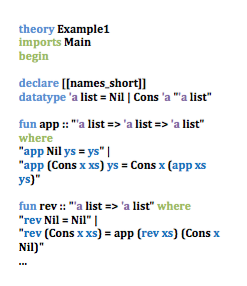
\includegraphics[width=.3\textwidth]{chapters/theoremprovers/isabelle1.png}
\end{figure}

\begin{figure}
\centering
\caption{Isabelle Proof 2}
\label{fig:isabelle2}
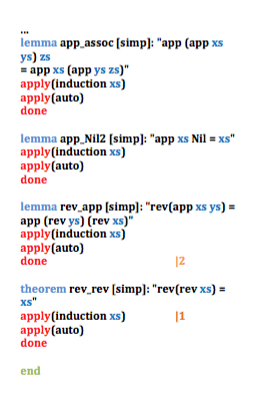
\includegraphics[width=.3\textwidth]{chapters/theoremprovers/isabelle2.png}
\end{figure}

\begin{figure}
\centering
\caption{Isabelle Antworten}
\label{fig:isabelle3}
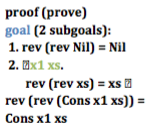
\includegraphics[width=.15\textwidth]{chapters/theoremprovers/isabelle3.png}
\end{figure}

\begin{figure}
\centering
\caption{Isabelle akzeptierter Beweis}
\label{fig:isabelle4}
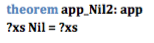
\includegraphics[width=.2\textwidth]{chapters/theoremprovers/isabelle4.png}
\end{figure}

\subsubsection*{Variante 2}
In \cref{fig:isabelle5} sieht man ein Beispiel, in dem der Beweis eigenhändig durchgeführt wird. Gezeigt werden soll, das Abbildungen von einer Menge in ihre Potenzmenge niemals surjektiv sein können. Ohne genau zu wissen wie die neuen Begriffe, wie assume, from, have und show anzuwenden sind, kann man den Beweis doch bereits recht leicht lesen.
In \cref{fig:isabelle6} sieht man, wie sich der Beweisstatus in |3 verändert hat, nach der Annahme, dass f surjektiv sei. Es wird ein f festgehalten, das Goal hat sich nicht verändert.
In \cref{fig:isabelle7} sieht man die Ausgabe von Isabelle, bevor das Lemma akzeptiert wird (|4).

\begin{figure}
\centering
\caption{Isabelle Beweis}
\label{fig:isabelle5}
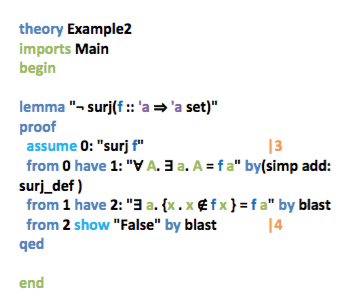
\includegraphics[width=.3\textwidth]{chapters/theoremprovers/isabelle5.png}
\end{figure}

\begin{figure}
\centering
\caption{Isabelle Beweisstatus}
\label{fig:isabelle6}
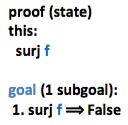
\includegraphics[width=.15\textwidth]{chapters/theoremprovers/isabelle6.png}
\end{figure}

\begin{figure}
\centering
\caption{Isabelle Status vor Lemma}
\label{fig:isabelle7}
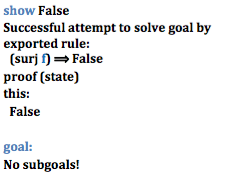
\includegraphics[width=.3\textwidth]{chapters/theoremprovers/isabelle7.png}
\end{figure}

\subsection{Automatisierte Theorembeweiser und DPLL(T)}
Nachdem wir nun die interaktiven Theorembeweiser kennen gelernt haben, schauen
wir uns die automatisierten etwas genauer an.
Wir unterscheiden unter anderem
zwei Methoden bei der automatisierten Beweissuche, den Davis-Putnam-Logeman-Loveland Algorithmus (kurz DPLL, auch DPLL(T) wobei T für Theorie steht) und das
Tableaukalkül (auch Baumkalkül, bzw. engl. Method of analytic tableaux).
Beide Herangehensweisen arbeiten auf einer Prädikatenlogik, allerdings sei das Baumkalkül
nur als weiterer Vertreter mit aufgeführt.
Grundlegend wird bei diesem versucht die
 Gegenaussage zu widerlegen.


\section{Schlusswort}
Nachdem wir nun einen Einblick in der Welt der TB erhalten haben und in Grundzügen wissen was TB sind und wie sie arbeiten sollen folgend einige Anwendungen vorgestellt werden.
Da Computerprogramme in verschiedenen Sprachen geschrieben werden, welche ein Vokabular, eine Grammatik und eine Syntax haben, können diese genauso für den theoretischen Inhalt her halten, wie mathematische Probleme.
Ein Beispiel dafür ist der Beweis des Vier-Farben-Satzes von Neil Robertson, Daniel P. Sanders, Paul Seymour und Robin Thomas, welcher genau genommen zwei Beweise beinhaltet.
Der erste zeigt, das der benutzte Algorithmus richtig arbeitet, also verifiziert die Korrektheit und der zweite, dass das Theorem gilt.
In der Wirtschaft setzt man Theorembeweiser vor allem für die Verifikation von integrierten Schaltkreisen und Prozessoren ein, z.B. um kritische Operationen zu prüfen.
Allerdings finden sie auch in Fachübergreifenden Gebieten ihren Nutzen. Insgesamt scheinen sie bei der Programmverifikation einer zunehmenden Beliebtheit zu unterliegen.
Der seL4 Mikrokernel, welcher in unzähligen Mobilgeräten vorkommt, wurde zum Beispiel mithilfe von Isabelle geprüft und seine Korrektheit nachgewiesen.
In der Mathematik sind sie noch sehr umstritten und auch wenn die vorhandenen Beweiser mächtige Werkzeuge sind, so können sie ihren menschlichen Kollegen heute noch nicht das Wasser reichen.
Eine naheliegende Anwendung diesbezüglich wäre nämlich das Erschaffen von neuen Theoremen und dabei bringen sie höchstens Triviale Aussagen zustande.
Mit \enquote{Automated Theorem Discovery}~\cite{Gao2014} richtet man den Blick auf das Schaffen von neuem Wissen, was allerdings noch in den Kinderschuhen steckt.
Das sogenannte \enquote{Theory-Exploration} hingegen versucht Möglichkeiten zu verwirklichen, um dem Anwender von interaktiven TB, im Falle des Feststeckens, mit Lemmas und Ideen weiter zu helfen.
Man bedenke, heutige TB zeigen nur, was noch nicht bewiesen ist und nicht, wie man solches zeigen kann.
Als Fazit kann man sagen, dass mit dieser Arbeit die Themengebiete gerade einmal angekratzt werden konnte, denn es gibt noch mehr als genug Ungesagtes zu den Theorembeweisern.
Mir persönlich hat die Arbeit von Thomas C. Hales über den Formalen Beweis sehr gut gefallen, da sie zeitgleich einen guten überblick verschafft.
Ich hatte darüber hinaus ein großes Interesse daran Isabelle einmal kennenzulernen und einen interaktiven TB selbst auszuprobieren.
Auch wenn die Zeit nicht gereicht hat um elegante Beweise zu führen, so konnte man doch zumindest einen Eindruck gewinnen.
Der Internetauftritt von Isabelle~\cite{isabellewebpage} bietet diesbezüglich gut verständliche Tutorials an, die für Interessierte in jedem Fall empfehlenswert sind.

\chapterimage{chapter_head_1.png}

\chapter{Bayessche Netze}
\section{Intro}
Ein Bayessches Netz stellt die Wahrscheinlichkeiten von Ereignissen und deren Abhängigkeit (bzw. Unabhängigkeit) zueinander dar.

Bayessche Netze finden immer dort Anwendungsmöglichkeit, wo Logik und Unwissenheit aufeinandertreffen.
Sie dienen der Vereinfachung von komplexen Problemen mit Hilfe weniger stochastischer Regeln.

In der Praxis finden Bayessche Netze beispielsweise in der Spracherkennung, medizinischen Diagnose, Filtern von Spam, Bildverarbeitung, Analyse von Kaufverhalten und in vielen anderen Gebieten Anwendung.

\begin{figure}[h]
    \centering
    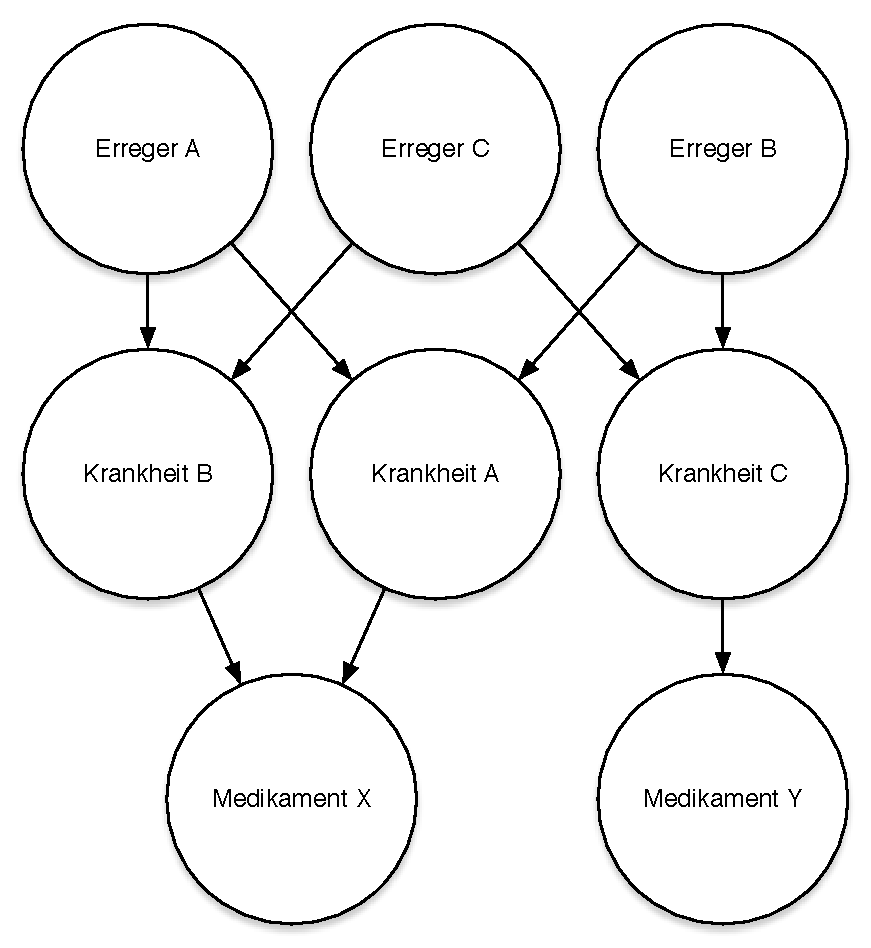
\includegraphics[width=.4\textwidth]{chapters/bayes/bayes_intro.pdf}
    \caption{Beispiel eines Bayesschen Netzes zur Diagnose von Krankheiten (ohne Wahrscheinlichkeiten)}
\end{figure}

\section{Grundlagen der Wahrscheinlichkeitsrechnung}
Einem Ereignis A weisen wir eine Wahrscheinlichkeit p(A) zwischen 0 (tritt nie ein) und 1 (tritt immer ein) zu.

Als marginal probability bezeichnen wir eine Wahrscheinlichkeit p(A), welche keine Abhängigkeiten aufweist.
Beispiel: A = Eine aus einem Skatdeck gezogene Karte ist Kreuz.
p(A) = 1/4 (oder 25~\%)

Als joint probability bezeichnen wir Wahrscheinlichkeiten, welche nebeneinander auftreten. p(A,B)
Beispiel: A (von oben) und B: Die Karte ist ein Bube

Da A und B voneinander unabhängige Ereignisse sind folgt:
p(A,B) = p(A) $\cdot$ p(B) = 1/8 $\cdot$ 1/4 = 1/32

Sind Ereignisse jedoch nicht unabhängig, so müssen wir die Wahrscheinlichkeit von p(A,B) bereits bestimmt haben.
Möchten wir nun für eine große Anzahl Ereignisse Wahrscheinlichkeiten berechnen, so benötigen wir extrem viele Daten.

\begin{center}
\begin{tabular}{ ccccc } \toprule
Sonne scheint & Werktag & Stau & Rasensprinkler & Tage im Jahr \\ \midrule
F & F & F & F & 4 \\
F & F & F & T & 5 \\
F & F & T & F & 2 \\
F & F & T & T & 1 \\
F & T & F & F & 13 \\
F & T & F & T & 2 \\
F & T & T & F & 66 \\
F & T & T & T & ... \\
T & F & F & F & ... \\
T & F & F & T & \\
T & F & T & F & \\
T & F & T & T & \\
T & T & F & F & \\
T & T & F & T & \\
T & T & T & F & \\
T & T & T & T & Errechenbar \\
\bottomrule
\end{tabular}
\end{center}


Bis auf 1 errechenbares Ergebnis benötigen wir die direkten Werte aller Kombinationen.
Wir benötigen also Für N Ereignisse $2^N-1$ Datensätze.
Gerade in der Medizin aus dem Anfangsbeispiel gibt es aber oft extrem viele Ereignisse.

Oftmals ist vieles davon aber auch nicht interessant, bzw. ableitbar.
Die Wahrscheinlichkeit, dass die Sonne scheint ist beispielsweise unabhängig davon ob der Tag ein Werktag ist.

Um die benötigten Datensätze möglichst gering zu halten betrachtet man bedingte Wahrscheinlichkeiten (conditional probability).

\section{Bedingte Wahrscheinlichkeit}
Bedingte Wahrscheinlichkeiten beruhen auf Annahmen.
Man nimmt etwa an, dass die Sonne keinen Einfluss auf die Frage hat, ob es nun ein Werktag ist, sehr wohl jedoch auf die Frage, ob der Sprinkler angeschaltet ist.
Gehen wir weiterhin davon aus, dass an sonnigen Tagen mehr Staus zustande kommen, da z.B. Fahrer geblendet werden.
Zudem gehen wir davon aus, dass werktags mehr Staus auftreten.
Fügen wir zudem noch das Verpassen des Essens hinzu, welches lediglich vom Stau abhängt.

\begin{figure}[h]
    \centering
    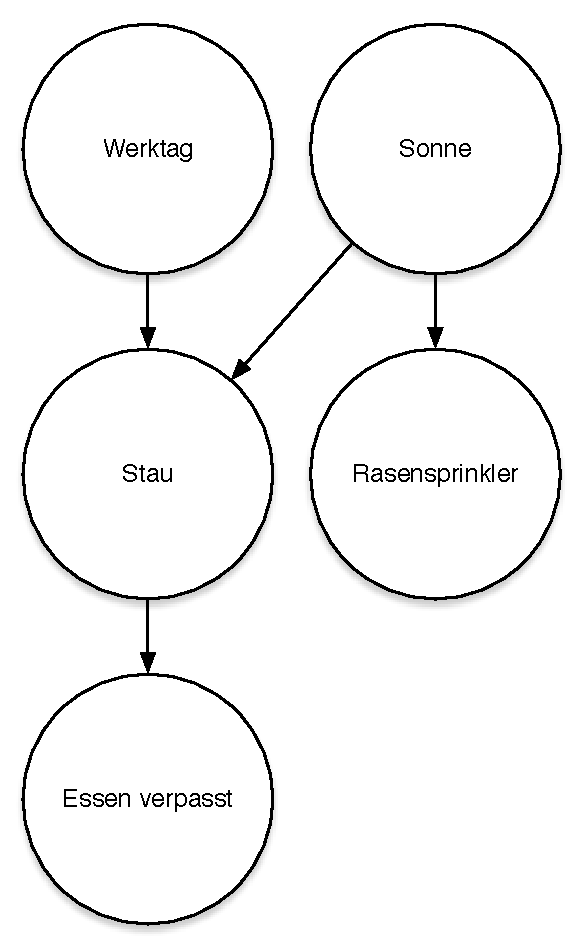
\includegraphics[width=.2\textwidth]{chapters/bayes/bayes_example.pdf}
\end{figure}

Unsere benötigten Datensätze mit fiktivem Inhalt:\\
$p(Sonne) = 0,8$\\
$p(Werktag)= 0,7$\\
$p(Rasensprinkler | Sonne) = 0,95$\\
$p(Rasensprinkler | !Sonne) = 0,20$\\
$p(Stau | Sonne,Werktag) = 0,8$\\
$p(Stau | !Sonne, Werktag) = 0,75$\\
$p(Stau | Sonne, !Werktag) = 0,15$\\
$p(Stau | !Sonne, !Werktag) = 0,05$\\
$p(Essen verpasst | Stau) = 0,5$\\
$p(Essen verpasst | !Stau) = 0,05$\\

Von 31 Datensätzen in einer Tabelle mit joint probabilities haben wir nun nur noch 10 benötigt Wahrscheinlichkeiten und können alle anderen nun problemlos errechnen. (Beispiel folgt)

Um bedingte Wahrscheinlichkeiten effektiv nutzen zu können benötigen wir einige Definitionen:
\begin{equation*}
p(A,B) = p (A | B) \cdot p (B)
\end{equation*}
Daraus folgt direkt:
\begin{equation*}
p(A,B,C) = p(A | B,C) \cdot p(B,C) = p(A | B,C) \cdot p(B | C) \cdot p(C)
\end{equation*}
Dies lässt sich für N Ereignisse wie folgt darstellen (Chain Rule):
\begin{equation*}
    P\left(\bigcap_{k=1}^N A_k\right)  = \prod_{k=1}^N  \mathrm P\left(A_k \,\Bigg|\, \bigcap_{j=1}^{k-1} A_j\right)
\end{equation*}
Zudem bezeichnen wir A als von B unabhängig, wenn gilt:
\begin{equation*}
p(A | B) = p(A)
\end{equation*}
und A als von B unabhängig unter der Prämisse C, wenn gilt:
\begin{equation*}
p(A | C) \cdot p(B | C) = p(A,B | C)
\end{equation*}

Mit Hilfe der Chain-Rule können wir nun für das Beispiel von oben jede mögliche joint probability ausrechnen.

Beispiel:
p(Essen verpasst,Stau,Werktag,Rasensprinkler,Sonne)
nach Anwendung der Chain Rule haben wir:
p(Essen verpasst | Stau,Werktag,Rasensprinkler,Sonne) \\ $\cdot$ p(Stau | Werktag , Rasensprinkler, Sonne) \\ $\cdot$ p(Werktag | Rasensprinkler, Sonne)
\\ $\cdot$ p( Rasensprikler | Sonne)
\\ $\cdot$ p(Sonne)

Wichtig ist hier den Aufbau des ersten Ausdrucks entlang der Abhängigkeiten zu formulieren. Die Reihenfolge der Ereignisse für die joint probabilty muss also eine umgedrehte topologische Anordnung unseres Graphen darstellen bzw. ein Ereignis A kann nicht vor einem Ereignis B stehen, wenn B abhängig von A ist.

Nach dem kürzen der Unabhängigkeiten erhalten wir:
p(Essen verpasst | Stau ) $\cdot$ p( Stau | Werktag, Sonne) $\cdot$ p( Werktag) $\cdot$ p( Rasensprinkler | Sonne) $\cdot$ p(Sonne)

Man nennt dies auch die Faktorisierung.

Die gesuchten Wahrscheinlichkeiten kennen wir bereits und können sie einsetzen:
0,5 $\cdot$ 0,8 $\cdot$ 0,7 $\cdot$ 0,95 $\cdot$ 0,8 = 0,218.

Es ist also durch simples Einsetzen unserer 10 Werte möglich sämtliche 31 Werte für die joint probability Tabelle zu berechnen.
Gleichzeitig sind Lösungen für relevante Fragen zur bedingten Wahrscheinlichkeit, welche nicht alle Ereignisse umfassen, mit geringem Aufwand zu lösen.


In der Regel sind jedoch nicht alle Angaben bekannt.
Nehmen wir nun an, dass wir als hart arbeitender Mensch an einem Nicht-Werktag zur Arbeit fahren und es sonnig ist.
Wir möchten nun wissen, wie wahrscheinlich es ist, dass man es abends bei der Rückfahrt rechtzeitig zum Essen schafft.
Wir suchen also p(!Essen verpasst | !Werktag, Sonne).

Dazu berechnen wir:
p(!Essen verpasst | Stau) $\cdot$ p(Stau | Sonne, Werktag) + p(!Essen verpasst | !Stau) $\cdot$ p(!Stau | Sonne, Werktag)

Die passenden Werte kennen wir entweder oder können sie direkt ableiten.
p(Essen verpasst | Stau) = 0,5
p(Essen verpasst | !Stau) = 0,05
p(Stau | Sonne, !Werktag) = 0,15

0,5 $\cdot$ 0,15 + 0,95 $\cdot$ 0,85 = 0,8825 bzw. die Wahrscheinlichkeit am Wochenende pünktlich zum Essen zu kommen ist 88\%.

Was jedoch, wenn ich in die andere Richtung rechnen möchte?
Beispiel: Der Lebensgefährte kommt pünktlich zum Essen und ich möchte Wissen, wie wahrscheinlich es ist, dass er im Stau gesteckt hat.

Wir kennen bereits die Formel:\\
p(A,B) = p (A | B) $\cdot$ p(B) offensichtlich gilt auch\\
p(B,A) = p (B | A) $\cdot$ p(A) wir folgern daraus:\\
p(A | B) = p(A,B) / P(B) = p(B,A) / P(B) = p(B | A) $\cdot$ p(A)/p(B) (Satz von Bayes)

Wir wissen also:
p(Stau | !Essen verpasst) = p(!Essen verpasst | Stau ) *P(Stau)/p(! Essen verpasst)

p(!Essen verpasst | Stau) =0,5\\
p(Stau) =\\
p(Stau | Sonne, Werktag) $\cdot$ p(Sonne) $\cdot$ p(Werktag) + \\ p(Stau | Sonne, !Werktag) $\cdot$ p(Sonne) $\cdot$ p(!Werktag)+ \\ p(Stau | !Sonne, Werktag) $\cdot$ p(!Sonne) $\cdot$ p(Werktag) + \\ p(Stau | !Sonne, !Werktag) $\cdot$ p(!Sonne) $\cdot$ p(!Werktag)\\ = 0,382

p(!Essen verpasst) =\\
p(!Essen verpasst | Stau) $\cdot$ p(Stau)\\ + p(!Essen verpasst | !Stau) $\cdot$ p(!Stau)\\ = 0,7781

$\Rightarrow$ p(Stau | !Essen verpasst)=0,5 $\cdot$ 0,382/0,7781 = 0,2454...

Ist die Person also pünktlich, so gab es mit einer Wahrscheinlichkeit von ~75\% keinen Stau.

An dieser Stelle ist anzufügen, dass das ganze Problem auch so hätte modelliert werden können, dass die Pünktlichkeit beim Essen ebenfalls vom Werktag abhängig ist, dann jedoch wäre die Abhängigkeit zum Stau zu hinterfragen, wenn es denn keinen Werktag gibt.
Es gibt also durchaus komplexere Problemstellungen, die wir mit unseren einfachen Methoden nicht so einfach behandeln können und eventuell verschiedene Modelle für Abhängigkeiten die je nach der Menge der Daten möglicherweise nicht optimal sind.

Diese neue Methode hilft uns vor allen Dingen damit mit einem einzelnen Modell gleichzeitig z.B. Krankheiten und Symptome in beide Richtungen zu bestimmen. Ohne große Umstände kann eine Krankheit aus Symptomen bestimmt werden und direkt von der Wahrscheinlichkeit der Krankheit kann die Wahrscheinlichkeit für weitere Symptome berechnet werden.

\section{Graphische Darstellung}
\begin{figure}[h]
    \centering
    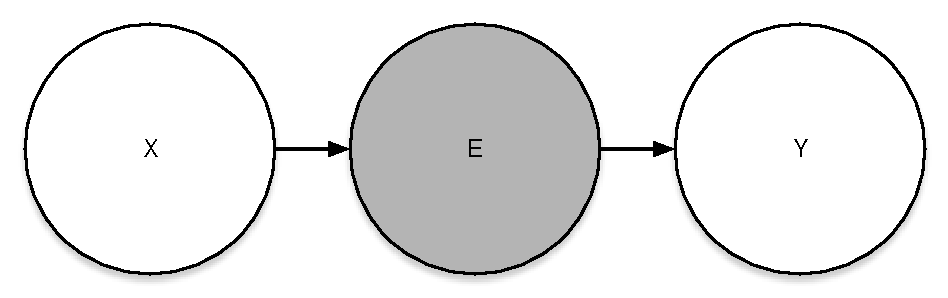
\includegraphics[width=.2\textwidth]{chapters/bayes/bayes_net_1.pdf}
\end{figure}
\begin{figure}[h]
    \centering
    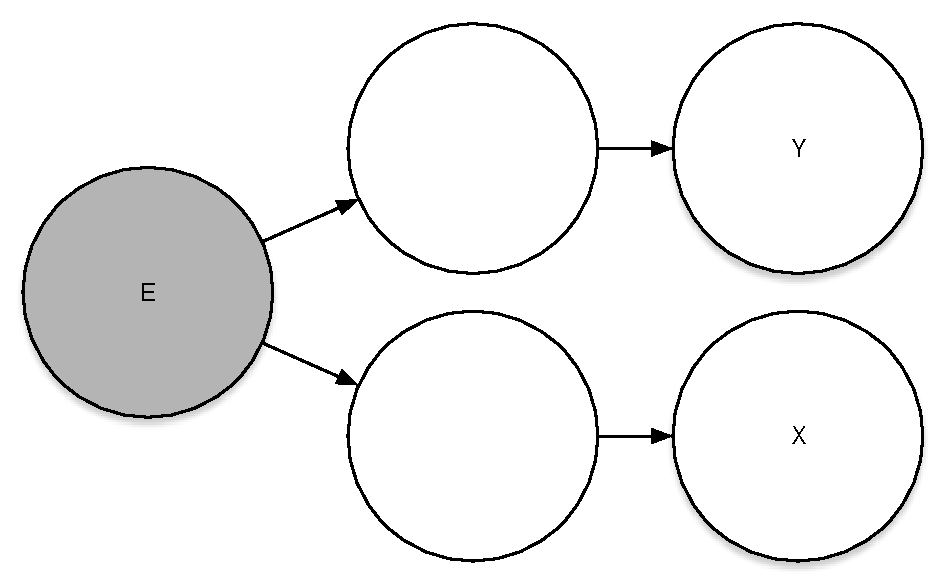
\includegraphics[width=.2\textwidth]{chapters/bayes/bayes_net_2.pdf}
\end{figure}
\begin{figure}[h]
    \centering
    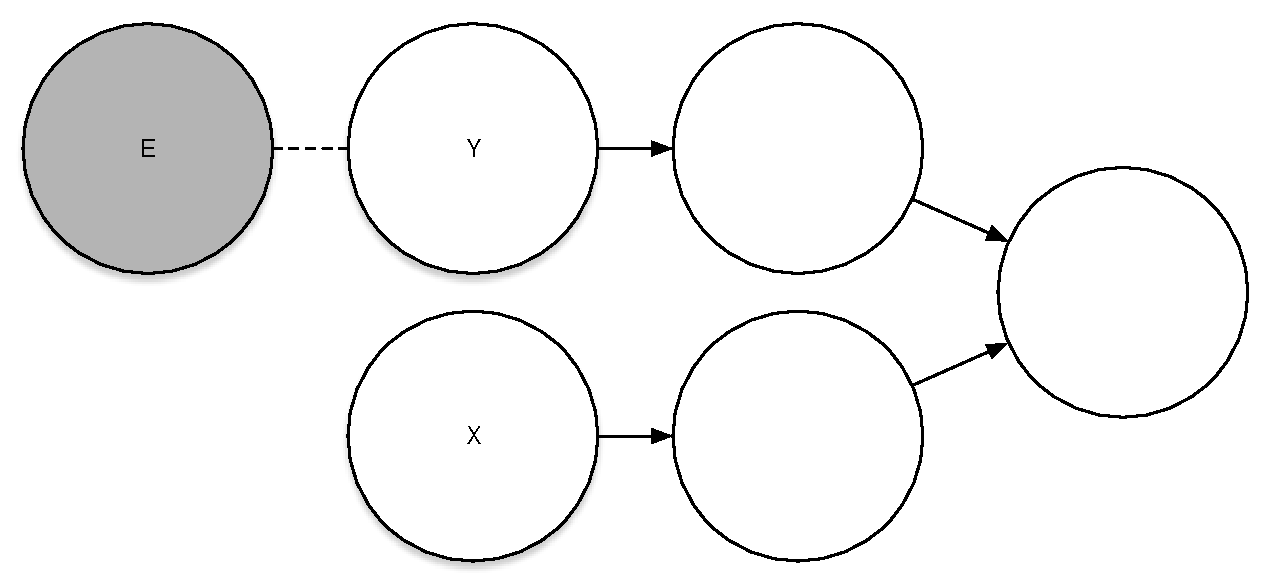
\includegraphics[width=.2\textwidth]{chapters/bayes/bayes_net_3.pdf}
\end{figure}
\begin{figure}[h]
    \centering
    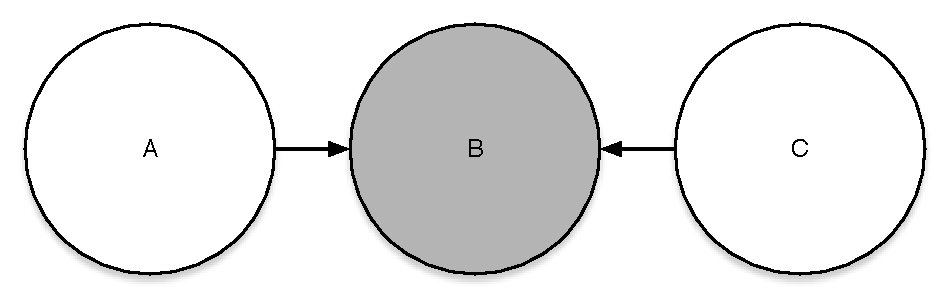
\includegraphics[width=.2\textwidth]{chapters/bayes/bayes_net_4.pdf}
\end{figure}

Wir nennen zwei Ereignisse X und Y bedingt unabhängig gegeben E, wenn im Graphen kein Weg von X zu Y existiert, welcher nicht E nicht beinhaltet.
Dies wir auch d-Separation genannt.
Wir schreiben hierfür
$X \perp Y | E$
Ausgehend vom vorherigen Beispiel heißt das, dass das Verpassen des Essens zwar vom Werktag abhängt, jedoch wenn bekannt ist, ob es einen Stau gab, diese Abhängigkeit aufgehoben wird.
Für 3 verknüpfte Ereignisse gibt es die Folgenden Möglichkeiten:
\begin{enumerate}[label=(\alph*)]
\item $A \rightarrow B \rightarrow C$ impliziert $A \perp C | B$
\item $A \leftarrow B \leftarrow C$ impliziert $A \perp C | B$
\item $A \leftarrow B \rightarrow C$ impliziert $A \perp C | B$
\item $A \rightarrow B \leftarrow C$ impliziert $A \perp C$
\end{enumerate}
Das Beispiel (d) beschreibt hierbei eine sogenannte V-Struktur.

Betrachten wir hierzu außerdem die Verschiedenen Faktorisierungen:
\begin{enumerate}[label=(\alph*)]
\item p(A,B,C) = p(C|B) $\cdot$ p(B|A) $\cdot$ p(A)
\item p(A,B,C) = p(A|B) $\cdot$ p(B|C) $\cdot$ p(C)
\item p(A,B,C) = p(A|B) $\cdot$ p(C|B) $\cdot$ p(B)
\item p(A,B,C) = p(B|A,C) $\cdot$ p(A) $\cdot$ p(C)
\end{enumerate}

\section{IC-Algorithmus}
Der IC Algorithmus ist eine Möglichkeit aus gegebenen Unabhängigkeiten ein Bayessches Netz zu erstellen.
\begin{enumerate}
\item Konstruiere einen ungerichteten Graphen; füge jede mögliche Kante (X,Y), für die es keine (bedingte) Abhängigkeit $X \perp Y | E$ bzw. $X \perp Y$ gibt, in den Graphen ein.
\item Gilt für zwei Nachbarn X,Y von einem Knoten E die bedingte Unabhängigkeit $X \perp Y | E$, dann füge die Kanten (X,E) und (Y,E) hinzu. (V-Struktur)
\item Orientiere die verbleibenden Kanten beliebig, aber ohne neue V-Strukturen entstehen zu lassen.
\end{enumerate}

\section{Quellen}
\begin{itemize}
\item Open Course „Artifical Intelligence“ am MIT
\item https://upload.wikimedia.org/math/b/5/a/b5a87dba9ec79dd6a93628c85fab ca97.png
\item http://www.informatik.uni-bremen.de/tdki/lehre/ss12/bayes/Intro.pdf
\item http://www.fil.ion.ucl.ac.uk/~wpenny/bdb/bayes.pdf
\item Bayesian Artificial Intelligence, Second Edition
\end{itemize}


\part{Suche}
\chapterimage{chapter_head_1.png}

\chapter{Tiefensuche, Beam-Seach und Hill Climbing}

\tikzset{
  treenode/.style = {align=center, inner sep=0pt, text centered,
    font=\sffamily},
  arn_n/.style = {treenode, circle, white, font=\sffamily\bfseries, draw=black,
    fill=black, text width=1.5em},% arbre rouge noir, noeud noir
  arn_r/.style = {treenode, circle, red, draw=red,
    text width=1.5em, very thick},% arbre rouge noir, noeud rouge
  arn_x/.style = {treenode, rectangle, draw=black,
    minimum width=0.5em, minimum height=0.5em}% arbre rouge noir, nil
}

\algnewcommand\algorithmicinput{\textbf{Input:}}
\algnewcommand\INPUT{\item[\algorithmicinput]}

\lstset{language=Haskell,frame=single,basicstyle=\small\ttfamily,numbers=left,firstnumber=1}
\lstset{language=Prolog,frame=single,basicstyle=\small\ttfamily,numbers=left,firstnumber=1}

\section{Motivation}

Die Hauptaufgabe von Rechnern ist, Probleme zu lösen. Oft kann man die Probleme graphisch darstellen, mit einem Start- und einem Zielknoten und die Wege zwichen den beiden. Hierfür benötigt man nicht nur eine Darstellung des aktuellen Zustandes sondern auch die Möglichkeiten, die zur Verfügung stehen, um das Ziel zu erreichen. Meistens gibt es keine einfache Lösung, denn nicht alle Probleme sind Addition von zwei positiven ganzen Zahlen. Daher benötigt man Suchverfahren. Hier beschänken wir uns auf die Depth-First Search, Breadth-First Search, Hill Climbing und Best-First Suchverfahren.

\section{Suchalgorithmen}

Wenn man vom Problem und der Darstellung abstrahiert, kann man die Suche nach einer Lösung in einem gerichteten Graph betrachten. Der gerichtete Graph wird nicht gegeben  sondern wird durch Erzeugungsregeln abgeleitet. Der Graph kann auch unendlich groß sein und daher ist die Suche und partielle Erzeugung des Graphen somit verflochten.

Unser Suchgraph besteht hier aus Knoten, die die Zustände beschreiben, und Kanten, in Form von Funktionen, die die Nachfolgerknoten berechnet. Außerdem definieren wir eine Anfangssituation und ein Ziel.

\begin{tikzpicture}[->,>=stealth',level/.style={sibling distance = 5cm/#1,level distance = 1.5cm}]
\node [arn_n] {S}
    child{ node [arn_n] {}
            child{ node [arn_n] {}
            	child{ node [arn_n] {}}
							child{ node [arn_x] {}}
            }
            child{ node [arn_n] {}
							child{ node [arn_n] {}}
							child{ node [arn_x] {}}
            }
    }
    child{ node [arn_n] {}
            child{ node [arn_n] {}
							child{ node [arn_n] {Z}}
							child{ node [arn_n] {}}
            }
            child{ node [arn_n] {}
							child{ node [arn_n] {}}
							child{ node [arn_x] {}}
            }
    };

    \node [below=5.2cm, align=flush center,text width=8cm]
       {
           Fig1: Graphische Darstellung eines Problems   S: Startknoten, Z: Zielknoten
       };
\end{tikzpicture}

%\subsection{Problemstellung}

%\TODO: Beispiel: Route finding, VLSI Layout, Assembly Sequencing

\section{Uninformierte Suche}
Wir betrachten zunächst die nicht informierte Suche. Hierbei wird bei der Suche nur den Graphen und die Nachfolgerfunktion berücksichtigt, aber keine anderen Informationen über die Knoten, Kanten usw. dürfen verwendet werden.

Die Paramenter für unseren Graph sind

\begin{itemize}
  \item Menge der initialen Knoten
  \item Menge der Zielknoten, bzw eindeutige Festlegung der Eigenschaft der Zielknoten
  \item Nachfolgerfunktion N
\end{itemize}

damit lässt sich folgender Algorithmus schreiben:

\begin{algorithm}
\caption{General-Search Algorithm}
\begin{algorithmic}[1]
\Function{General-Search}{problem,strategy} \State \textbf{returns} a solution, or failure
\State initialize the search tree using the initial state of $problem$
\Loop \State choose a leaf node for expansion according to $strategy$
  \If {there are no candidates for expansion}{failure}
  \If{the node contains a goal state}{the corresponding solution}
  \Else{expand the node and add the resulting nodes to the search tree}
\EndLoop
\EndFunction
\end{algorithmic}
\end{algorithm}


Wir betrachten im folgenden Varianten der blinden Suche, die insbesondere das Wählen des Knotens eindeutig durchführen.

\subsection{Depth-First Search}
Die Depth-First Suche verwendet eine Liste von Knoten und wählt als nächsten zu betrachtenden Knoten dieser Liste. Außerdem werden neue Nachfolger vorne in die Liste eingefügt, was zur Charakteristik führt, dass zunächst in der Tiefe gesucht wird.

\begin{algorithm}
\caption{Depth-First Search Algorithm}
\begin{algorithmic}[1]
\Function{Depth-First-Search}{problem} \State \textbf{returns} a solution, or failure
\Function{General-Search}{problem,Enqueue-At-Front}
\EndFunction
\EndFunction
\end{algorithmic}
\end{algorithm}

Die Depth-First Suche eignet sich damit besonders für Suchbäume, deren Äste eine vertretbare Länge nicht überschreiten.

\begin{tikzpicture}[->,>=stealth',level 1/.style={sibling distance=50mm},level 2/.style={sibling distance=20mm},level 3/.style={sibling distance=12mm},
%scale=1.2, transform shape
]
\node (nA)[arn_n] {A}
   child { node (nB)[arn_n] {B}
              child { node (nD) [arn_n] {D}
                         child { node (nH) [arn_n] {H} }
                       }
              child {  node (nE) [arn_n] {E}
                         child { node (nI) [arn_n] {I} }
                         child { node (nJ) [arn_n] {J} }
                       }
            }
   child { node (nC) [arn_n] {C}
              child { node (nF) [arn_n] {F}
                         child { node (nK) [arn_n] {K}  }
                         child { node (nL) [arn_n] {L} }
                         child { node (nM) [arn_n] {M} }
                       }
              child {  node (nG) [arn_n] {G} }
             };

  \draw[->,blue,rounded corners,dashed,line width=0.7pt]
    ($(nA) + (-0.4,0.2)$) --
    ($(nB) +(-0.3,0.4)$) --
    ($(nB) +(-0.6,0.0)$) --
    ($(nD)  +(-0.4,0.3)$) --
    ($(nD)  +(-0.5,0.0)$) --
    ($(nH)  +(-0.5,0.0)$) --
    ($(nH)  +(-0.4,-0.35)$) --
    ($(nH)  +(0.0,-0.5)$) --
    ($(nH)  +(0.4,-0.35)$) --
    ($(nH)  +(0.5,0.0)$) --
%    ($(nD)  +(0.45,-0.2)$) --
    ($(nD)  +(0.45,0.0)$) --
    ($(nB)  +(0.0,-0.4)$) --
    ($(nE)  +(-0.45,0.0)$) --
    ($(nI)  +(-0.45,0.0)$) --
    ($(nI)  +(-0.35,-0.35)$) --
    ($(nI)  +(0.0,-0.45)$) --
    ($(nI)  +(0.35,-0.35)$) --
    ($(nI)  +(0.4,0.0)$) --
    ($(nE)  +(0.0,-0.4)$) --
    ($(nJ)  +(-0.45,0.0)$) --
    ($(nJ)  +(-0.35,-0.35)$) --
    ($(nJ)  +(0.0,-0.45)$) --
    ($(nJ)  +(0.35,-0.35)$) --
    ($(nJ)  +(0.45,0.0)$) --
    ($(nE)  +(0.4,0.2)$) --
    ($(nB)  +(0.4,0.0)$) --
    ($(nA)  +(0.0,-0.4)$) --
    ($(nC)  +(-0.4,0.0)$) --
%    ($(nF)  +(-0.6,0.0)$) --
    ($(nK)  +(-0.5,0.1)$) --
    ($(nK)  +(-0.4,-0.35)$) --
    ($(nK)  +(0.0,-0.5)$) --
    ($(nK)  +(0.4,-0.3)$) --
    ($(nF)  +(-0.15,-0.4)$) --
    ($(nL)  +(-0.5,0.0)$) --
    ($(nL)  +(-0.4,-0.35)$) --
    ($(nL)  +(0.0,-0.5)$) --
    ($(nL)  +(0.4,-0.35)$) --
    ($(nL)  +(0.5,0.0)$) --
    ($(nF)  +(0.15,-0.4)$) --
    ($(nM)  +(-0.5,0.0)$) --
    ($(nM)  +(-0.4,-0.35)$) --
    ($(nM)  +(0.0,-0.5)$) --
    ($(nM)  +(0.4,-0.35)$) --
    ($(nM)  +(0.5,0.2)$) --
    ($(nF)  +(0.4,0.0)$) --
    ($(nC)  +(0.0,-0.4)$) --
    ($(nG)  +(-0.5,0.0)$) --
    ($(nG)  +(-0.4,-0.35)$) --
    ($(nG)  +(0.0,-0.5)$) --
    ($(nG)  +(0.4,-0.35)$) --
    ($(nG)  +(0.5,0.1)$) --
    ($(nC) +(0.6,0.0)$) --
    ($(nC) +(0.3,0.4)$) --
    ($(nA) + (0.4,0.2)$);

    \node [below=5.4cm, align=flush center,text width=8cm]
       {
           Fig2: Graphische Darstellung der Depth-First Suche
       };
\end{tikzpicture}

Eine mögliche Implementierung der Depth-First Suche in Prolog ist:


\lstinputlisting[language=Prolog]{chapters/dfs/tiefensuche.pl}

Und in Haskell:

\lstinputlisting[language=Haskell]{chapters/dfs/tiefensuche.hs}

Die explizite Speicherung der Pfade sowohl in Haskell als auch in Prolog kostet nicht viel Effizienz. Man kann den Algorithmus auch in imperativen Sprachen implementieren, indem jeder Eintrag einen Knoten mit Zeiger auf den nächsten Nachbarknoten zugeordnet wird. Die Komplexität des Verfahrens (worst-case) für die Zeit ist entsprechend der Anzahl der besuchten Knoten exponentiell in der Tiefe und für den Speicherplatz linear bei fester Verzweigungsrate.

Das Problem bei der Depth-First Suche ist, dass der Algorithmus nicht vollständig ist. Wenn der Suchgraph unendlich groß ist, kann die Suche am Ziel vorbeilaufen und für immer im unendlichen langen Pfad laufen.

Um dies zu verbeugen kann man eine Tiefenbeschränkung (k) einbauen. Wenn die vorgegebene Tiefenschrank (k) überschriten wird, werden keine Nachfolger dieser Knoten mehr erzeugt. Die Depth-First Suche findet in diesem Fall jeden Zielknoten, der höchstens Tiefe k hat.

Wenn der gerichtete Graph kein Baum ist, kann man auch die schon untersuchten Knoten in einer Hash-Tabelle speichern und somit werden die Knoten nicht nochmal untersucht sondern redundant weiterverfolgt.

Hierfür ist der Platzbedarf entsprechend der Anzahl der besuchten Knoten und die Berechnungszeit gleich $n*log(n)$ mit n = Anzahl der untersuchten Knoten.

\subsubsection{Backtracking}
Die Arbeitsweise der Depth-First Suche ist: Wenn Knoten K keine Nachfolger hat (oder eine Tiefenbeschränkung) überschritten wurde, dann mache weiter mit dem nächsten Bruder von K. Ist der Pfad nicht erfolgreich, führt die Depth-First Suche Backtracking durch. Dies wird als chronologisches Zurücksetzen bezeichnet.

Es gibt auch Suchprobleme, bei denen kein Backtracking erforderlich ist (greedy Verfahren ist möglich) zum Beispiel, wenn jeder Knoten noch einen Zielknoten als Nachfolger hat. Die Depth-First Suche reicht dann aus, wenn die Tiefe der Zielknoten in alle Richtungen unterhalb jedes Knotens beschränkt ist. Anderenfalls reicht Depth-First Suche nicht aus, da ein Ast immer ausgesucht werden kann, indem der Zielknoten weiter weg ist.

\subsection{Breadth-First Search}
Die Breadth-First Suche verwendet auch eine Liste von Knoten wie bei der Depth-First Suche. Der Unterschied hierbei ist, dass die neuen Nachfolger hinten in die Liste eingefügt werden, was zur Charakteristik führt, dass zunächst in der Breite gesucht wird.

\begin{algorithm}
\caption{Breadth-First Search Algorithm}
\begin{algorithmic}[1]
\Function{Breadth-First-Search}{problem} \State \textbf{returns} a solution, or failure
\Function{General-Search}{problem,Enqueue-At-End}
\EndFunction
\EndFunction
\end{algorithmic}
\end{algorithm}

Die Breadth-First Suche untersucht somit ausgehend von Startknoten alle Nachbarknoten. Ist der Zielknoten noch nicht erreicht, werden alle Nachbarknoten der bisher untersuchten Knoten betrachtet.

\begin{tikzpicture}[->,>=stealth',level 1/.style={sibling distance=50mm},level 2/.style={sibling distance=20mm},level 3/.style={sibling distance=12mm},
%scale=1, transform shape
]
\node (nA)[arn_n] {A}
   child { node (nB)[arn_n] {B}
              child { node (nD) [arn_n] {D}
                         child { node (nH) [arn_n] {H} }
                       }
              child {  node (nE) [arn_n] {E}
                         child { node (nI) [arn_n] {I} }
                         child { node (nJ) [arn_n] {J} }
                       }
            }
   child { node (nC) [arn_n] {C}
              child { node (nF) [arn_n] {F}
                         child { node (nK) [arn_n] {K}  }
                         child { node (nL) [arn_n] {L} }
                         child { node (nM) [arn_n] {M} }
                       }
              child {  node (nG) [arn_n] {G} }
             };

  \draw[->,blue,rounded corners,dashed,line width=0.7pt]
    ($(nA) + (-0.4,0.2)$) --
    ($(nB) +(-0.3,0.4)$) --
    ($(nB) +(-0.6,0.0)$) --
    ($(nC)  +(+0.3,0.2)$) --
    ($(nC)  +(+0.6,0.0)$) --
    ($(nD)  +(-0.3,0.4)$) --
    ($(nD)  +(-0.4,0.0)$) --
    ($(nE)  +(0.0,0.0)$) --
    ($(nE)  +(0.0,0.0)$) --
    ($(nF)  +(0.0,0.0)$) --
    ($(nF)  +(0.0,0.0)$) --
    ($(nG)  +(0.3,0.2)$) --
    ($(nG)  +(+0.6,0.0)$) --
    ($(nH)  +(-0.3,0.4)$) --
    ($(nH)  +(0.0,0.0)$) --
    ($(nI)  +(0.0,0.0)$) --
    ($(nI)  +(0.0,0.0)$) --
    ($(nJ)  +(0.0,0.0)$) --
    ($(nJ)  +(0.0,0.0)$) --
    ($(nK)  +(0.0,0.0)$) --
    ($(nK)  +(0.0,0.0)$) --
    ($(nL)  +(0.0,0.0)$) --
    ($(nL)  +(0.0,0.0)$) --
    ($(nM)  +(+0.5,0.0)$);

    \node [below=5.2cm, align=flush center,text width=8cm]
       {
           Fig3: Graphische Darstellung der Breadth-First Suche
       };
\end{tikzpicture}

Eine mögliche Implementierung der Breadth-First Suche in Prolog ist:

\lstinputlisting[language=Prolog]{chapters/dfs/breitensuche.pl}

Und in Haskell:

\lstinputlisting[language=Haskell]{chapters/dfs/breitensuche.hs}

Die Vor- und Nachteile der Breadth-First Suche lässt sich wie folgt zusammenfassen:

\begin{itemize}
  \item Die Breadth-First Suche ist vollständig. Das bedeutet, wenn es eine Lösung gibt, wird sie mit Sicherheit gefunden.
  \item Der kürzeste Weg wird gefunden, dafür wird aber viel Speicherplatz benötigt.
  \item Es werden Knoten besucht, die für den optimalen Pfad nicht besucht werden müssten. Damit wird auch der Zeitaufwand erhöht. Dies beträgt nämlich $n+n*log(n)$, für n = Anzahl der Knoten.
\end{itemize}

\subsection{Reverse Search}
Bei der Rückwärtssuche wird von einem (bekannten) Zielknoten ausgegangen in die Richtung des Anfangsknoten.

Voraussetzungen für die Rückwärtssuche sind:

\begin{itemize}
  \item Der Zielknoten kann explizit angeben werden(nicht nur eine Eigenschaft, die der Zielknoten erfüllen muss).
  \item Von jedem Knoten ist es möglich, die direkten Vorgänger zu berechnen.
\end{itemize}

Reverse Suche ist aber nur besser als Vorwärtssuche, wenn die Verzweigungsrate in Rückwärtsrichtung kleiner ist als die Verzweigungsrate in Vorwärtsrichtung. Das Problem an der Reverse Suche ist oft, dass die Vorgängerfunktion schwer zu finden ist.

\section{Informierte Suche}

Die Algorithmen, die bis jetzt betrachtet wurden, erzeugen neuen Zuständen und vergleichen sie immer wieder mit dem Zielzustand, bis sie übereinstimmen. Diese Strategie funktioniert, ist aber oft sehr kostenaufwendig. Wir betrachten im folgenden heuristischen Algorithmen.

Die Suche wird als \enquote{heuristische} oder \enquote{informierte} bezeichnet, wenn man zusätzlich zu den Knoten und zu der Datenstruktur eine Schätzfunktion gibt, die als Schätzung des Abstands zum Zielknoten interpretieren werden kann. Der Zielknoten sollte ein Maximum bzw. Minimum der Schätzfunktion sein.

Eine Heuristik ist dann eine Methode, die oft ihren Zweck erreicht, aber nicht mit Sicherheit. Man spricht von heuristischer Suche, wenn die Schätzfunktion in vielen praktisch brauchbaren Fällen die richtige Richtung zu einem Ziel angibt, aber möglicherweise manchmal versagt.

Wir suchen dann das Maximum (oder Mininum) einer Knotenfunktion auf einem gerichteten Graphen.

\subsection{Hill Climbing}
Der Hill Climbing Suchalgorithm ist auch als Gradientenaufstieg bekannt, da die Suche immer in Richtung der Vergrößerung einer Funktion läuft.

Parameter, die notwendig für den Algorithmus sind:

\begin{itemize}
  \item die Menge der initialen Knoten,
  \item die Nachfolgerfunktion,
  \item die Schätzfunktion,
  \item und der Zieltest.
\end{itemize}

Der Algorithmus verhält sich wie die Depth-First Suche, wobei der Nachfolger, der zu expandieren ist, nach der Schätzfunktion ausgesucht wird.

\begin{algorithm}
\caption{Hill Climbing Algorithm}
\begin{algorithmic}[1]
\Function{Hill-Climbing}{problem} \State \textbf{returns} a solution state
\INPUT
\Statex $problem$ \Comment Ein Problem
\Statex $current$  \Comment Ein Knoten
\Statex $next$  \Comment Ein Knoten
\State $current \gets Make-Node(Initial-State[problem])$
\Loop
\State $next \gets$ größter Wert aus $current$
\If{$VALUE[next] < VALUE[current]$}{\Return current}
\State $current \gets next$
\EndLoop
\EndFunction
\end{algorithmic}
\end{algorithm}


Das Problem bei dem Hill Climbing Algorithmus ist, dass er bei lokalen Maxima abbricht. Es ist möglich, in dem Hill-Clinbing Algorithmus Zyklen einzubauen, damit Backtracking durchgeführt wird, aber er bleibt eine zeitlang in den Maxima hängen.

Wenn mehrere Nachfolger die gleiche Schätzwerte haben, ist der Weg, den ausgesucht werden soll, nicht eindeutig.

Eine mögliche Implementierung der Hill Climbing Suche in Haskell ist:

\lstinputlisting[language=Haskell]{chapters/dfs/hillclimbing.hs}

\subsection{Best-First-Search}
Die Best-First-Suche wählt immer den Knoten aus, der den besten Wert bzgl. der Schätzfunktion hat. Der Knoten wird dann überprüft und, wenn der nicht das Ziel ist, expandiert.


\begin{algorithm}
\caption{Best-First-Search Algorithm}
\begin{algorithmic}[1]
\Function{Best-First-Search}{problem,EVAL-FN} \State \textbf{returns} a solution sequence
\INPUT
\Statex $problem$ \Comment Ein Problem
\Statex $Eval-Fn$  \Comment Eine Evaluationsfunktion
\State $Queueing-Fn \gets$ a function that orders nodes by EVAL-FN
\State \textbf{return} GENERAL-SEARCH(problem, Queueing-Fn)
\EndFunction
\end{algorithmic}
\end{algorithm}


Eine Implementierung der Best-First Suche in Haskell ist:

\lstinputlisting[language=Haskell]{chapters/dfs/bestfirst.hs}

Die Best-First-Suche ist mit der Depth-First Suche eng verbunden. Der Unterschied ist, dass bei der Best-First Suche den nächsten Knoten, der überprüft und expandiert wird, mithilfe der Schätzfunktion ausgesucht wird. Dabei werden alle Knoten im Stack bewertet und dadurch können lokale Maxima schnell verlassen werden.

Wie bei der Depth-First Suche ist die Best-First Suche hier nicht vollständig und die Platzkosten steigern exponentiell in der Tiefe.

\section{Fazit \& Bewertung}
Zunächst wurden das Suchproblem und der Begriff \enquote{Suche} erläutert. Die nicht informierte Suchverfahren wurden präsentiert und es wurde gezeigt, dass ein General Search Algorithmus alle Probleme löst, wenn die richtige Strategie ausgesucht wird.
Tiefensuche bedeutet, dass man beginnend im Startknoten so weit wie möglich entlang der bestehenden Kanten in die Tiefe geht, ehe man zurückläuft und dann in bislang unbesuchte Teilbäume absteigt.
Breitensuche bedeutet, dass man beginnend im Startknoten alle direkt verbundenen Knoten besucht, bevor die nächst tiefere Ebene überprüft wird.
Die Vollständigkeit und die Komplexität der gängigen uninformierten Suchalgorithmen wurden erläutert.
Dabei ist klar geworden, dass die Zeit- und Speicherplatzkosten hoch sind.

Um die Kosten zu minimieren werden die bekannte Suchverfahren weiterentwickelt. Daraus folgte zum Beispiel die Best-First Suche. Diese ist eine General Search, wobei nur die minimale Anzahl der Knoten berücksichtigt wird.

Solche Algorithmen, wobei die Kosten minimiert werden, nennen wir \textbf{greedy Algorithmen}. Der Algorithmus ist aber immer noch nicht optimal.

\section{Quellen und Literatur}

\begin{itemize}
\item Stuart J. Russel and Peter Norvig, “Artificial Intelligence - A Modern Approach”, Pretince Hall, Englewood Cliffs, New Jersey 2010
\item Ivan Bratko, “Prolog Programming for Artificial Intelligence”, Addison-Wesley Yugoslavia 1990
\item R. Schenk and R.P. Abelson, “Scripts, Plans and Knowledge”, International Joint Conference on Artificial Intelligence, 1975
\item F.C. Pereira and S.M.Schieber, “Prolog and Natural-Language Analysis”, CSLI, 1987
\item F.M. Donini, M. Lenzerini and others, “The complexity of concept languages”, Inf. Comput., 1997
\item I. Wegener, “Highlights aus der Informatik”, Springer, Berlin, 1996
\item MIT Open Course - Artificial Intelligence
 \url{http://ocw.mit.edu/courses/electrical-engineering-and-computer-science/6-034-artificial-intelligence-fall-2010/}, Zugriff 28.04.2016
\end{itemize}

\chapterimage{chapter_head_1.png}

\chapter{Informierte Suche}
\section{Beispiel}

Wir wollen nun den $\text{A}^*$ Algorithmus an einem Beispiel anwenden.
Sei dazu der Graph $G$ und die Heuristik $h$ durch
\fbox{
\begin{tikzpicture}[auto, node distance=2cm, every loop/.style={},
                    thick,main node/.style={circle,draw,font=\sffamily\Large\bfseries}]

  \node[main node, label={\color{red}\small 9}] (1) at (1, 3) {1};
  \node[main node, label={\color{red}\small 6}] (2) at (4, 3) {2};
  \node[main node, label={\color{red}\small 7}] (3) at (3, 4) {3};
  \node[main node, label={\color{red}\small 5}] (4) at (5, 4) {4};
  \node[main node, label=left:{\color{red}\small 5}] (5) at (5, 1) {5};
  \node[main node, label={\color{red}\small 1}] (6) at (9, 3) {6};
  \node[main node, label={\color{red}\small 2}] (7) at (8, 4) {7};
  \node[main node, label=left:{\color{red}\small 2}] (8) at (8, 1) {8};
  \node[main node, label={\color{red}\small 8}] (9) at (2, 1) {S};
  \node[main node, label={\color{red}\small 0}] (10) at (10, 2) {Z};

  \path[every node/.style={font=\sffamily\small}]
  (9) edge node [sloped, below] {2.5} (1)
  (1) edge node [sloped] {3} (2)
  (2) edge node [sloped, above] {4.5} (7)
  (7) edge node [left, yshift=0.5cm] {3} (8)
  (8) edge node [sloped, above] {2.5} (10)
  (9) edge node [sloped] {3.5} (3)
  (3) edge node [sloped] {2} (4)
  (4) edge node [right] {3} (5)
  (5) edge node [sloped] {4.5} (6)
  (6) edge node [sloped, above] {1.5} (10)
  (4) edge node [sloped, above] {1.5} (2);

\end{tikzpicture}}\vspace{5pt}\\
gegeben. Wir wollen einen Weg von $S$ nach $Z$ suchen. Man erhält Folgendes:
(hierbei ist eine Zahl im Knoten rot, falls er in der Extended-List
ist, grün wenn er gerade expandiert wird und gelb falls er auf der Open-List
ist):\vspace{5pt}\\
\fbox{
\begin{tikzpicture}[auto, node distance=2cm, every loop/.style={},
                    thick,main node/.style={circle,draw,font=\sffamily\Large\bfseries}]

  \node[main node, label={\color{red}\small 9}] (1) at (1, 3) {1};
  \node[main node, label={\color{red}\small 6}] (2) at (4, 3) {2};
  \node[main node, label={\color{red}\small 7}] (3) at (3, 4) {3};
  \node[main node, label={\color{red}\small 5}] (4) at (5, 4) {4};
  \node[main node, label=left:{\color{red}\small 5}] (5) at (5, 1) {5};
  \node[main node, label={\color{red}\small 1}] (6) at (9, 3) {6};
  \node[main node, label={\color{red}\small 2}] (7) at (8, 4) {7};
  \node[main node, label=left:{\color{red}\small 2}] (8) at (8, 1) {8};
  \node[main node, color=green, label={\color{red}\small 8}] (9) at (2, 1) {S};
  \node[main node, label={\color{red}\small 0}] (10) at (10, 2) {Z};

  \path[every node/.style={font=\sffamily\small}]
  (9) edge node [sloped, below] {2.5} (1)
  (1) edge node [sloped] {3} (2)
  (2) edge node [sloped, above] {4.5} (7)
  (7) edge node [left, yshift=0.5cm] {3} (8)
  (8) edge node [sloped, above] {2.5} (10)
  (9) edge node [sloped] {3.5} (3)
  (3) edge node [sloped] {2} (4)
  (4) edge node [right] {3} (5)
  (5) edge node [sloped] {4.5} (6)
  (6) edge node [sloped, above] {1.5} (10)
  (4) edge node [sloped, above] {1.5} (2);

\end{tikzpicture}}
\hfill
\fbox{\begin{minipage}[b][4.27cm][t]{0.34\textwidth}
    \begin{tabular}{|l|r|}
      Queue & Prio\\
      (S) & 8\\
      \phantom{(S, 3, 4, 5, 6, Z)} & \phantom{14.5}
    \end{tabular}
\end{minipage}}\vspace{5pt}\\
\fbox{
\begin{tikzpicture}[auto, node distance=2cm, every loop/.style={},
                    thick,main node/.style={circle,draw,font=\sffamily\Large\bfseries}]

  \node[main node, color=yellow, label={\color{red}\small 9}] (1) at (1, 3) {1};
  \node[main node, label={\color{red}\small 6}] (2) at (4, 3) {2};
  \node[main node, color=green, label={\color{red}\small 7}] (3) at (3, 4) {3};
  \node[main node, label={\color{red}\small 5}] (4) at (5, 4) {4};
  \node[main node, label=left:{\color{red}\small 5}] (5) at (5, 1) {5};
  \node[main node, label={\color{red}\small 1}] (6) at (9, 3) {6};
  \node[main node, label={\color{red}\small 2}] (7) at (8, 4) {7};
  \node[main node, label=left:{\color{red}\small 2}] (8) at (8, 1) {8};
  \node[main node, color=red, label={\color{red}\small 8}] (9) at (2, 1) {S};
  \node[main node, label={\color{red}\small 0}] (10) at (10, 2) {Z};

  \path[every node/.style={font=\sffamily\small}]
  (9) edge node [sloped, below] {2.5} (1)
  (1) edge node [sloped] {3} (2)
  (2) edge node [sloped, above] {4.5} (7)
  (7) edge node [left, yshift=0.5cm] {3} (8)
  (8) edge node [sloped, above] {2.5} (10)
  (9) edge node [sloped] {3.5} (3)
  (3) edge node [sloped] {2} (4)
  (4) edge node [right] {3} (5)
  (5) edge node [sloped] {4.5} (6)
  (6) edge node [sloped, above] {1.5} (10)
  (4) edge node [sloped, above] {1.5} (2);

\end{tikzpicture}}\hfill
\fbox{\begin{minipage}[b][4.27cm][t]{0.34\textwidth}
    \begin{tabular}{|l|r|}
      Queue & Prio\\
      (S, 3) & 10\\
      (S, 1) & 11.5\\
      \phantom{(S, 3, 4, 5, 6, Z)} & \phantom{14.5}
    \end{tabular}
\end{minipage}}
\vspace{5pt}\\
\fbox{
\begin{tikzpicture}[auto, node distance=2cm, every loop/.style={},
                    thick,main node/.style={circle,draw,font=\sffamily\Large\bfseries}]

  \node[main node, color=yellow, label={\color{red}\small 9}] (1) at (1, 3) {1};
  \node[main node, label={\color{red}\small 6}] (2) at (4, 3) {2};
  \node[main node, color=red, label={\color{red}\small 7}] (3) at (3, 4) {3};
  \node[main node, color=green, label={\color{red}\small 5}] (4) at (5, 4) {4};
  \node[main node, label=left:{\color{red}\small 5}] (5) at (5, 1) {5};
  \node[main node, label={\color{red}\small 1}] (6) at (9, 3) {6};
  \node[main node, label={\color{red}\small 2}] (7) at (8, 4) {7};
  \node[main node, label=left:{\color{red}\small 2}] (8) at (8, 1) {8};
  \node[main node, color=red, label={\color{red}\small 8}] (9) at (2, 1) {S};
  \node[main node, label={\color{red}\small 0}] (10) at (10, 2) {Z};

  \path[every node/.style={font=\sffamily\small}]
  (9) edge node [sloped, below] {2.5} (1)
  (1) edge node [sloped] {3} (2)
  (2) edge node [sloped, above] {4.5} (7)
  (7) edge node [left, yshift=0.5cm] {3} (8)
  (8) edge node [sloped, above] {2.5} (10)
  (9) edge node [sloped] {3.5} (3)
  (3) edge node [sloped] {2} (4)
  (4) edge node [right] {3} (5)
  (5) edge node [sloped] {4.5} (6)
  (6) edge node [sloped, above] {1.5} (10)
  (4) edge node [sloped, above] {1.5} (2);

\end{tikzpicture}}\hfill
\fbox{\begin{minipage}[b][4.27cm][t]{0.34\textwidth}
    \begin{tabular}{|l|r|}
      Queue & Prio\\
      (S, 3, 4) & 10\\
      (S, 1) & 11.5\\
      \phantom{(S, 3, 4, 5, 6, Z)} & \phantom{14.5}
    \end{tabular}
\end{minipage}}\vspace{5pt}\\
\fbox{
\begin{tikzpicture}[auto, node distance=2cm, every loop/.style={},
                    thick,main node/.style={circle,draw,font=\sffamily\Large\bfseries}]

  \node[main node, color=green, label={\color{red}\small 9}] (1) at (1, 3) {1};
  \node[main node, color=yellow, label={\color{red}\small 6}] (2) at (4, 3) {2};
  \node[main node, color=red, label={\color{red}\small 7}] (3) at (3, 4) {3};
  \node[main node, color=red, label={\color{red}\small 5}] (4) at (5, 4) {4};
  \node[main node, color=yellow, label=left:{\color{red}\small 5}] (5) at (5, 1) {5};
  \node[main node, label={\color{red}\small 1}] (6) at (9, 3) {6};
  \node[main node, label={\color{red}\small 2}] (7) at (8, 4) {7};
  \node[main node, label=left:{\color{red}\small 2}] (8) at (8, 1) {8};
  \node[main node, color=red, label={\color{red}\small 8}] (9) at (2, 1) {S};
  \node[main node, label={\color{red}\small 0}] (10) at (10, 2) {Z};

  \path[every node/.style={font=\sffamily\small}]
  (9) edge node [sloped, below] {2.5} (1)
  (1) edge node [sloped] {3} (2)
  (2) edge node [sloped, above] {4.5} (7)
  (7) edge node [left, yshift=0.5cm] {3} (8)
  (8) edge node [sloped, above] {2.5} (10)
  (9) edge node [sloped] {3.5} (3)
  (3) edge node [sloped] {2} (4)
  (4) edge node [right] {3} (5)
  (5) edge node [sloped] {4.5} (6)
  (6) edge node [sloped, above] {1.5} (10)
  (4) edge node [sloped, above] {1.5} (2);

\end{tikzpicture}}\hfill
\fbox{\begin{minipage}[b][4.27cm][t]{0.34\textwidth}
    \begin{tabular}{|l|r|}
      Queue & Prio\\
      (S, 1) & 11.5\\
      (S, 3, 4, 2) & 13\\
      (S, 3, 4, 5) & 13.5\\
      \phantom{(S, 3, 4, 5, 6, Z)} & \phantom{14.5}
    \end{tabular}
\end{minipage}}\vspace{5pt}\\
\fbox{
\begin{tikzpicture}[auto, node distance=2cm, every loop/.style={},
                    thick,main node/.style={circle,draw,font=\sffamily\Large\bfseries}]

  \node[main node, color=red, label={\color{red}\small 9}] (1) at (1, 3) {1};
  \node[main node, color=green, label={\color{red}\small 6}] (2) at (4, 3) {2};
  \node[main node, color=red, label={\color{red}\small 7}] (3) at (3, 4) {3};
  \node[main node, color=red, label={\color{red}\small 5}] (4) at (5, 4) {4};
  \node[main node, color=yellow, label=left:{\color{red}\small 5}] (5) at (5, 1) {5};
  \node[main node, label={\color{red}\small 1}] (6) at (9, 3) {6};
  \node[main node, label={\color{red}\small 2}] (7) at (8, 4) {7};
  \node[main node, label=left:{\color{red}\small 2}] (8) at (8, 1) {8};
  \node[main node, color=red, label={\color{red}\small 8}] (9) at (2, 1) {S};
  \node[main node, label={\color{red}\small 0}] (10) at (10, 2) {Z};

  \path[every node/.style={font=\sffamily\small}]
  (9) edge node [sloped, below] {2.5} (1)
  (1) edge node [sloped] {3} (2)
  (2) edge node [sloped, above] {4.5} (7)
  (7) edge node [left, yshift=0.5cm] {3} (8)
  (8) edge node [sloped, above] {2.5} (10)
  (9) edge node [sloped] {3.5} (3)
  (3) edge node [sloped] {2} (4)
  (4) edge node [right] {3} (5)
  (5) edge node [sloped] {4.5} (6)
  (6) edge node [sloped, above] {1.5} (10)
  (4) edge node [sloped, above] {1.5} (2);

\end{tikzpicture}}\hfill
\fbox{\begin{minipage}[b][4.27cm][t]{0.34\textwidth}
    \begin{tabular}{|l|r|}
      Queue & Prio\\
      (S, 1, 2) & 11.5\\
      (S, 3, 4, 2) & 13\\
      (S, 3, 4, 5) & 13.5\\
      \phantom{(S, 3, 4, 5, 6, Z)} & \phantom{14.5}
    \end{tabular}
\end{minipage}}\vspace{5pt}\\
\fbox{
\begin{tikzpicture}[auto, node distance=2cm, every loop/.style={},
                    thick,main node/.style={circle,draw,font=\sffamily\Large\bfseries}]

  \node[main node, color=red, label={\color{red}\small 9}] (1) at (1, 3) {1};
  \node[main node, color=red, label={\color{red}\small 6}] (2) at (4, 3) {2};
  \node[main node, color=red, label={\color{red}\small 7}] (3) at (3, 4) {3};
  \node[main node, color=red, label={\color{red}\small 5}] (4) at (5, 4) {4};
  \node[main node, color=yellow, label=left:{\color{red}\small 5}] (5) at (5, 1) {5};
  \node[main node, label={\color{red}\small 1}] (6) at (9, 3) {6};
  \node[main node, color=green, label={\color{red}\small 2}] (7) at (8, 4) {7};
  \node[main node, label=left:{\color{red}\small 2}] (8) at (8, 1) {8};
  \node[main node, color=red, label={\color{red}\small 8}] (9) at (2, 1) {S};
  \node[main node, label={\color{red}\small 0}] (10) at (10, 2) {Z};

  \path[every node/.style={font=\sffamily\small}]
  (9) edge node [sloped, below] {2.5} (1)
  (1) edge node [sloped] {3} (2)
  (2) edge node [sloped, above] {4.5} (7)
  (7) edge node [left, yshift=0.5cm] {3} (8)
  (8) edge node [sloped, above] {2.5} (10)
  (9) edge node [sloped] {3.5} (3)
  (3) edge node [sloped] {2} (4)
  (4) edge node [right] {3} (5)
  (5) edge node [sloped] {4.5} (6)
  (6) edge node [sloped, above] {1.5} (10)
  (4) edge node [sloped, above] {1.5} (2);

\end{tikzpicture}}\hfill
\fbox{\begin{minipage}[b][4.27cm][t]{0.34\textwidth}
    \begin{tabular}{|l|r|}
      Queue & Prio\\
      (S, 1, 2, 7) & 12\\
      (S, 3, 4, 2) & 13\\
      (S, 3, 4, 5) & 13.5\\
      \phantom{(S, 3, 4, 5, 6, Z)} & \phantom{14.5}
    \end{tabular}
\end{minipage}}\vspace{5pt}\\
\fbox{
\begin{tikzpicture}[auto, node distance=2cm, every loop/.style={},
                    thick,main node/.style={circle,draw,font=\sffamily\Large\bfseries}]

  \node[main node, color=red, label={\color{red}\small 9}] (1) at (1, 3) {1};
  \node[main node, color=red, label={\color{red}\small 6}] (2) at (4, 3) {2};
  \node[main node, color=red, label={\color{red}\small 7}] (3) at (3, 4) {3};
  \node[main node, color=red, label={\color{red}\small 5}] (4) at (5, 4) {4};
  \node[main node, color=green, label=left:{\color{red}\small 5}] (5) at (5, 1) {5};
  \node[main node, label={\color{red}\small 1}] (6) at (9, 3) {6};
  \node[main node, color=red, label={\color{red}\small 2}] (7) at (8, 4) {7};
  \node[main node, color=yellow, label=left:{\color{red}\small 2}] (8) at (8, 1) {8};
  \node[main node, color=red, label={\color{red}\small 8}] (9) at (2, 1) {S};
  \node[main node, label={\color{red}\small 0}] (10) at (10, 2) {Z};

  \path[every node/.style={font=\sffamily\small}]
  (9) edge node [sloped, below] {2.5} (1)
  (1) edge node [sloped] {3} (2)
  (2) edge node [sloped, above] {4.5} (7)
  (7) edge node [left, yshift=0.5cm] {3} (8)
  (8) edge node [sloped, above] {2.5} (10)
  (9) edge node [sloped] {3.5} (3)
  (3) edge node [sloped] {2} (4)
  (4) edge node [right] {3} (5)
  (5) edge node [sloped] {4.5} (6)
  (6) edge node [sloped, above] {1.5} (10)
  (4) edge node [sloped, above] {1.5} (2);

\end{tikzpicture}}\hfill
\fbox{\begin{minipage}[b][4.27cm][t]{0.34\textwidth}
    \begin{tabular}{|l|r|}
      Queue & Prio\\
      (S, 3, 4, 5) & 13.5\\
      (S, 1, 2, 7, 8) & 15\\
      \phantom{(S, 3, 4, 5, 6, Z)} & \phantom{14.5}
    \end{tabular}\\
    Der Weg $(S, 3, 4, 2)$ wurde entfernt, da $2$ schon in der Closed-List ist.
\end{minipage}}\vspace{5pt}\\
\fbox{
\begin{tikzpicture}[auto, node distance=2cm, every loop/.style={},
                    thick,main node/.style={circle,draw,font=\sffamily\Large\bfseries}]

  \node[main node, color=red, label={\color{red}\small 9}] (1) at (1, 3) {1};
  \node[main node, color=red, label={\color{red}\small 6}] (2) at (4, 3) {2};
  \node[main node, color=red, label={\color{red}\small 7}] (3) at (3, 4) {3};
  \node[main node, color=red, label={\color{red}\small 5}] (4) at (5, 4) {4};
  \node[main node, color=red, label=left:{\color{red}\small 5}] (5) at (5, 1) {5};
  \node[main node, color=green, label={\color{red}\small 1}] (6) at (9, 3) {6};
  \node[main node, color=red, label={\color{red}\small 2}] (7) at (8, 4) {7};
  \node[main node, color=yellow, label=left:{\color{red}\small 2}] (8) at (8, 1) {8};
  \node[main node, color=red, label={\color{red}\small 8}] (9) at (2, 1) {S};
  \node[main node, label={\color{red}\small 0}] (10) at (10, 2) {Z};

  \path[every node/.style={font=\sffamily\small}]
  (9) edge node [sloped, below] {2.5} (1)
  (1) edge node [sloped] {3} (2)
  (2) edge node [sloped, above] {4.5} (7)
  (7) edge node [left, yshift=0.5cm] {3} (8)
  (8) edge node [sloped, above] {2.5} (10)
  (9) edge node [sloped] {3.5} (3)
  (3) edge node [sloped] {2} (4)
  (4) edge node [right] {3} (5)
  (5) edge node [sloped] {4.5} (6)
  (6) edge node [sloped, above] {1.5} (10)
  (4) edge node [sloped, above] {1.5} (2);

\end{tikzpicture}}\hfill
\fbox{\begin{minipage}[b][4.27cm][t]{0.34\textwidth}
    \begin{tabular}{|l|r|}
      Weg & Prio\\
      (S, 3, 4, 5, 6) & 14\\
      (S, 1, 2, 7, 8) & 15\\
      \phantom{(S, 3, 4, 5, 6, Z)} & \phantom{14.5}
    \end{tabular}
\end{minipage}}\vspace{5pt}\\
\fbox{
\begin{tikzpicture}[auto, node distance=2cm, every loop/.style={},
                    thick,main node/.style={circle,draw,font=\sffamily\Large\bfseries}]

  \node[main node, color=red, label={\color{red}\small 9}] (1) at (1, 3) {1};
  \node[main node, color=red, label={\color{red}\small 6}] (2) at (4, 3) {2};
  \node[main node, color=red, label={\color{red}\small 7}] (3) at (3, 4) {3};
  \node[main node, color=red, label={\color{red}\small 5}] (4) at (5, 4) {4};
  \node[main node, color=red, label=left:{\color{red}\small 5}] (5) at (5, 1) {5};
  \node[main node, color=red, label={\color{red}\small 1}] (6) at (9, 3) {6};
  \node[main node, color=red, label={\color{red}\small 2}] (7) at (8, 4) {7};
  \node[main node, color=yellow, label=left:{\color{red}\small 2}] (8) at (8, 1) {8};
  \node[main node, color=red, label={\color{red}\small 8}] (9) at (2, 1) {S};
  \node[main node, color=green, label={\color{red}\small 0}] (10) at (10, 2) {Z};

  \path[every node/.style={font=\sffamily\small}]
  (9) edge node [sloped, below] {2.5} (1)
  (1) edge node [sloped] {3} (2)
  (2) edge node [sloped, above] {4.5} (7)
  (7) edge node [left, yshift=0.5cm] {3} (8)
  (8) edge node [sloped, above] {2.5} (10)
  (9) edge node [sloped] {3.5} (3)
  (3) edge node [sloped] {2} (4)
  (4) edge node [right] {3} (5)
  (5) edge node [sloped] {4.5} (6)
  (6) edge node [sloped, above] {1.5} (10)
  (4) edge node [sloped, above] {1.5} (2);

\end{tikzpicture}}\hfill
\fbox{\begin{minipage}[b][4.27cm][t]{0.34\textwidth}
    \begin{tabular}{|l|r|}
      Weg & Prio\\
      (S, 3, 4, 5, 6, Z) & 14.5\\
      (S, 1, 2, 7, 8) & 15\\
      \phantom{(S, 3, 4, 5, 6, Z)} & \phantom{14.5}
    \end{tabular}\\
    Hier bricht Algorithmus ab, da $Z$ zu suchen war, und gibt
    $(S, 3, 4, 5, 6, Z)$ aus.
\end{minipage}}\vspace{5pt}\\
Somit ist $(S, 3, 4, 5, 6, Z)$ der kürzeste Weg von $S$ nach $Z$.

\chapterimage{chapter_head_1.png}

\chapter{Suchalgorithmen für Spiele}

\usetikzlibrary{calc}
\usetikzlibrary{positioning}
\usetikzlibrary{matrix}

\pgfdeclarelayer{background}
\pgfsetlayers{background,main}


\section{Intro \& Motivation}

In den vorangegangenen Kapiteln haben wir schon einige Suchverfahren kennengelernt, welche uns nun helfen werden Algorithmen zu verstehen, die verwendet werden um Computergegner für Nullsummenspiele zu entwickeln. Hierbei werden wir uns den Minimax-Algorithmus, sowie den Alpha-Beta-Algorithmus genauer anschauen, welche beide versuchen sich in die Lage des Gegners zu versetzen, um so  herauszufinden, welche Reaktion dieser auf einen Zug von uns wählen würde. Ziel der Algorithmen ist es, ein für uns best mögliches Ergebnis und somit, wenn möglich, einen Sieg zu erlangen. Dieses Vorgehen kann eine Betrachtung von sehr vielen möglichen Züge zur Folge haben, was sehr viel Rechenaufwand bedeutet. Im Folgenden werden wir jedoch  mit Hilfe des Alpha-Beta-Algorithmus eine Methode kennenlernen, die es uns ermöglicht die Anzahl der zu betrachtenden Züge zu reduzieren.



\section{Inhaltliche Ausarbeitung des Themas}

Wir betrachten ein Nullsummenspiel, was bedeutet, dass der Gewinn des einen Spielers (Nutzwert positiv) mit dem Verlust des Gegners (Nutzwert negativ) äquivalent ist und ein Unentschieden keine Auswirkungen auf die Nullsummeneigenschaft hat (Nutzwert 0).
Gegeben sei für dieses Spiel ein Spielbaum $T = (V;E)$. Bei einem gleichförmigen Spielbaum besitzt jeder innerer Knoten den gleichen Verzweigungsgrad b und alle Blätter befinden sich in der gleichen Tiefe d, , sodass die Zahl der Knoten in einem gleichförmigen Baum exponentiell mit der Tiefe des Baumes wächst ($b^d$). Jedoch gibt es auch Spielbäume bei denen der Verzweigungsgrad der Ebenen variiert.
Der Spielbaum beinhaltet alle möglichen Züge und Spielausgänge. Die Tiefe und der Verzweigungsgrad hängt von dem Spiel ab, welches wir betrachten. Beispielsweise hat der Spielbaum zu einem Tic-Tac-Toe Spiel eine Tiefe von 9 (da es 9 Felder zu besetzen gibt) und zu Beginn des Spiels einen Verzweigungsgrad von 9 (weil noch alle 9 Felder zur Auswahl stehen), der mit wachsender Tiefe allerdings abnimmt, da nach jedem Zug immer ein leeres Feld weniger vorhanden ist.



\subsection{Problemstellung}
Zu dem gegeben Nullsummenspiel wollen wir einen Computergegner programmieren, der in der Lage ist die optimale Antwort auf jede Spielposition, bei optimalem Spiel beider Spieler, zu finden.
Dafür müssen wir jedoch vorher festlegen, was für uns optimal in diesem Zusammenhang bedeutet. Wir gehen davon aus, dass der Gegner immer den für ihn optimalen Zug wählt, dh der Zug, der für ihn zum besten Nutzwert und somit für uns zum schlechtesten Nutzwert führt. Analog wollen wir agieren. Wie dies genau funktioniert werden wir im folgenden Abschnitt sehen.



\subsection{Methoden}


\subsubsection*{Minimax Algorithmus}
Im folgenden bezeichnen wir unseren Spieler mit MAX und den gegnerischen Spieler mit MIN. Wie zuvor schon angedeutet ist das Ziel des Minimax Algorithmus den Minimax-Wert für die aktuelle Stellung zu bestimmen. Der Minimax-Wert der Endstellungen (Blätter) entspricht dem Nutzwert für MAX. Die Berechnung der anderen Knoten erfolgt rekursiv mit Hilfe der folgenden Bewertungsfunktion:

\begin{center}
	$Minimax(k) = \begin{cases} Nutzwert(k) &		,falls~ k ~Endzustand\\
		max\{minimax(t) ~|~ t \in N(t)\} 	&		,falls~ k~ MAX-Knoten\\
		min\{minimax(t) ~|~ t \in N(t)\},	&		,falls~ k~ MIN-Knoten	\end{cases} $
\end{center}

wobei $N(t)$ die Funktion ist, die die Kinder im Baum liefert. Die Auswertung der Knoten geschieht Bottom up, das bedeutet wir beginnen bei den Blättern und bewerten von dort ausgehend die Elternknoten und anschließend deren Eltern bis wir irgendwann bei der Wurzel angelangt sind. Der Minimax Algorithmus liefert nicht unbedingt den höchsten Nutzwert der Blätter, sondern den größten Nutzwert den man erhalten kann, wenn der Gegner selbst versucht zu gewinnen und somit den Nutzwert für uns möglichst klein zu halten.\\

Anschaulicher wird das ganze, wenn man sich den Algorithmus an einem Beispiel anschaut.

\textbf{Beispiel}\\

Gegeben sei der folgende Spielbaum
\begin{center}
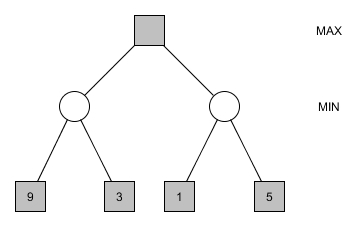
\includegraphics[width = 7 cm]{chapters/minimax/jpg/Graph-Minmax1.jpg}
\end{center}

Angenommen MIN wäre an der markierten Position:
\begin{center}
	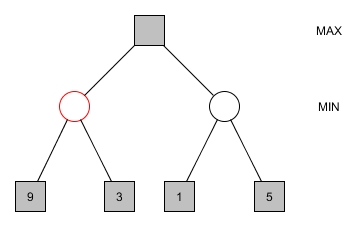
\includegraphics[width = 7 cm]{chapters/minimax/jpg/Graph-Minmax2-1.jpg}
\end{center}

Dann würde MIN den Zug auswählen, der für ihn den größten Nutzwert und somit für uns den kleinsten Nutzwert hat. Das heißt in dem Fall:
\begin{center}
	 $min\{minimax(t) | t \in N(t)\} ~=~ min\{9,3\} ~=~ 3$

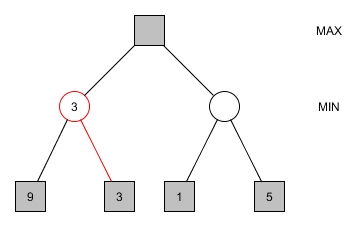
\includegraphics[width = 7 cm]{chapters/minimax/jpg/Graph-Minmax2-2.jpg}
\end{center}

Angenommen MIN wäre an der markierten Position:
\begin{center}
	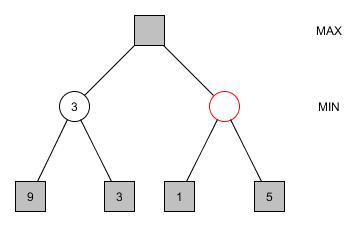
\includegraphics[width = 7 cm]{chapters/minimax/jpg/Graph-Minmax2-3.jpg}
\end{center}

Dann würde MIN den Zug auswählen, der für ihn den größten Nutzwert und somit für uns den kleinsten Nutzwert hat. Das heißt in dem Fall:
\begin{center}
	$min\{minimax(t) | t \in N(t)\} ~=~ min\{1,5\} ~=~ 1$

	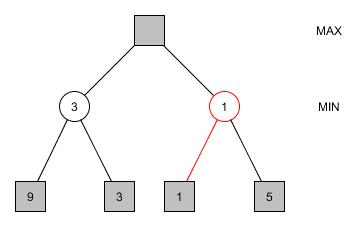
\includegraphics[width = 7 cm]{chapters/minimax/jpg/Graph-Minmax2-4.jpg}
\end{center}

Nun betrachten wir den Zug von MAX. Der Suchbaum sieht wie folgt aus

\begin{center}
	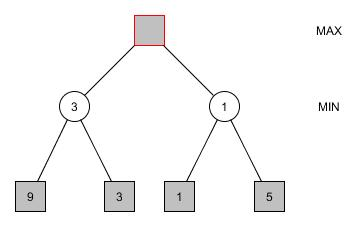
\includegraphics[width = 7 cm]{chapters/minimax/jpg/Graph-Minmax2.jpg}
\end{center}

MAX würde den Zug wählen, der für ihn den höchsten Nutzwert hat.\\

\begin{center}
	$max\{minimax(t) | t \in N(t)\} ~=~ max\{3,1\} ~=~ 3$
	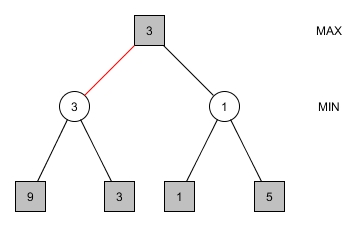
\includegraphics[width = 7 cm]{chapters/minimax/jpg/Graph-Minmax3.jpg}
\end{center}

Somit sieht der Suchbaum nach Abschluss des Minimax-Algorithmus wie folgt aus, wobei der rote Pfad den optimalsten Nutzwert liefert, wenn beide Spieler optimal spielen. Somit sollte MAX den linken Knoten wählen.

\begin{center}
	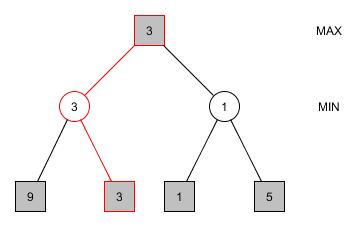
\includegraphics[width = 7 cm]{chapters/minimax/jpg/Graph-Minmax4.jpg}
\end{center}

\vskip 60pt



\subsubsection*{Problem:} Der Minimax-Algorithmus durchsucht den Suchbaum $T=(V, E)$ mit Tiefensuche, in der Zeit $O(max {|V|, |E|}) = O(|V|)$. Somit benötigt die Suche zwar lineare Zeit, jedoch wächst der Baum exponentiell mit zunehmender Tiefe ($O(|V|)=O(b^d)$). Somit ist der Algorithmus für Bäume mit großer Tiefe ineffizient.


\subsubsection*{Alpha-Beta-Algorithmus}
 Der Alpha-Beta-Algorithmus ist eine Verbesserung vom Minimax-Algorithmus, da die Zugriffsanzahl reduziert wird, indem Teile des Suchbaums nicht durchsucht werden, ohne dabei das Ergebnis zu verfälschen. Für die Umsetzung werden die Variablen $\alpha$ und $\beta$ eingeführt, wobei $\alpha$ der Nutzwert ist, welchen MAX mindestens erreicht und $\beta$ der Nutzwert, den MIN höchstens erreicht. Die Auswertung der Knoten geschieht on-the-fly, dh nur dann wenn wir sie wirklich benötigen. \\

 \underline{MAX-Knoten:}\\
 Betrachten wir einen MAX Knoten und stellen dort einen Wert fest der größer ist als $\beta$ brauchen wir den Teilbaum nicht weiter betrachten, da MIN diesen nicht wählen würde, weil der andere Teilbaum einen kleineren Nutzwert liefert. Das nicht weiter Betrachten des Teilbaums bezeichnet man als Beta-Cutoff. Ist  der Wert des MAX Knoten größer als $\alpha$ erhöht sich der Wert den MAX mindestens erreicht und wir aktualisieren $\alpha$ auf den Wert des Knotens.  \\

 \underline{MIN-Knoten:}\\
 Ist der Wert eines MIN Knotens kleiner als der Wert von $\alpha$ müssen wir diesen Teilbaum nicht weiter analysieren, da MAX immer den Teilbaum mit dem größten Nutzwert auswählt und da $\alpha$ größer ist als der Wert des betrachteten Knotens existiert ein Teilbaum mit einem größeren Nutzwert. Also würde hier ein Cutoff stattfinden, welchen man als Alpha-Cutoff bezeichnet. Sollte jedoch der Wert des MIN Knotens größer als $\beta$ sein steigt der Wert den MIN höchstens erreicht und wir müssen $\beta$ auf diesen Wert anpassen.


 \begin{algorithm}
 	\KwData{Graph $G=(V,E)$, Blätter mit Nutzwert, s = Knoten}
 	\KwResult{Nutzwert für jeden knoten}
 	\textbf{alpha-beta-suche(s)}\\

 	\textbf{return} maximalerWert(s, -$\infty$, $\infty$)\\

 	\textbf{maximalerWert}(Knoten, $\alpha$, $\beta$)\\

	 	\If{s = Blatt}{
	 		\textbf{return} wert(s)
	 	}
	 	\Else{
	 		$wert = \alpha$\\
	 		\lForEach{k= Kind(s)}{
		 		$wert = max\{wert, minimalerWert(k, wert, \beta)\}$\\
		 		\If {$wert >= \beta$}{
			 		\textbf{return} wert}
			 	$\alpha = max\{\alpha, wert\}$\\
	 		\textbf{return} wert
	 		}
	 	}

	\textbf{minimalerWert}(Knoten, $\alpha$, $\beta$)\\

	\If{s = Blatt}{
		\textbf{return} wert(s)
	}
	\Else{
		$wert = \beta$\\
		\lForEach{k= Kind(Knoten)}{
			$wert = min\{wert, minimalerWert(k, \alpha, wert)\}$\\
			\If {$wert <= \alpha$}{
				\textbf{return} wert}
			$\beta = min\{\beta, wert\}$\\
			\textbf{return} wert
		}
	}
 	\caption{Alhpa-Beta-Algorithmus}
\end{algorithm}

Betrachten wir ein Beispiel, um den Algorithmus besser zu verstehen.

\textbf{Beispiel:}\\

Gegeben sei der folgende Spielbaum:
\begin{center}
	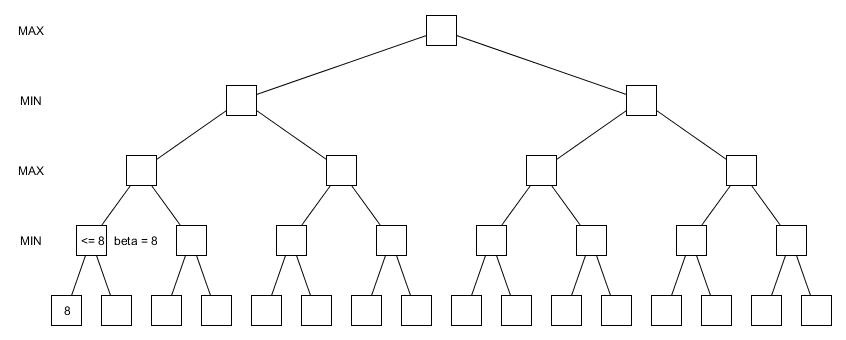
\includegraphics[width = 12 cm]{chapters/minimax/jpg/Alpha-beta1.jpg}
\end{center}

Wir betrachten das erste Blatt. Da MIN immer den Zug mit dem niedrigsten Nutzwert auswählt erreicht er einen Nutzwert $<=8$. Somit ist $\beta = 8$. Da $\beta > \alpha = -\infty$ müssen wir noch das andere Blatt betrachten.

\begin{center}
	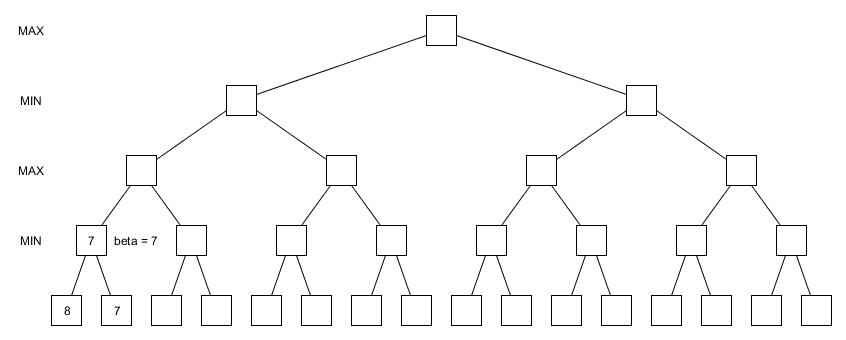
\includegraphics[width = 12 cm]{chapters/minimax/jpg/Alpha-beta2.jpg}
\end{center}

Das zweite Blatt hat den Nutzwert 7, somit ist er kleiner als der aktuelle Wert von $\beta$. Aus diesem Grund erhält der MIN-Knoten den Wert $min\{8,~7\} =7$. Somit ergibt sich für den darüberliegenden Knoten, dass er einen Wert $>=7$ hat, da MAX immer den Knoten mit dem größten Nutzwert auswählt. Nun betrachten wir das Blatt mit dem Nutzwert 3.

\begin{center}
	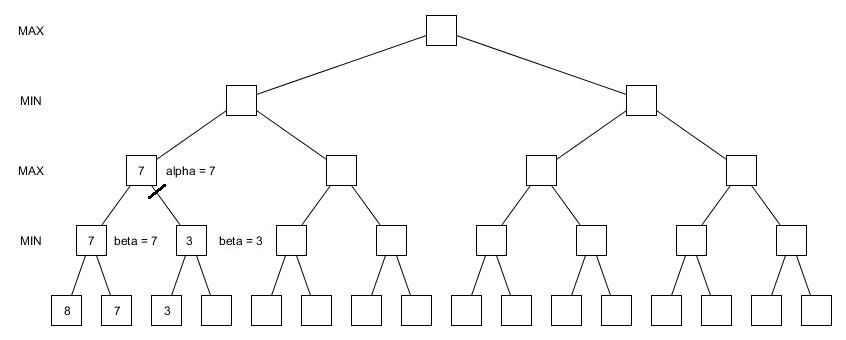
\includegraphics[width = 12 cm]{chapters/minimax/jpg/Alpha-beta3.jpg}
\end{center}

Sein Elternknoten hat für $\alpha$ den Wert 7 (MAX erreicht mind. eine 7) und $\beta$ hat den Wert 3 (MIN erreicht höchstens den Wert 3). Vergleicht man $\alpha$ und den Wert des MIN Knotens fällt auf, dass $\alpha$ > 3 was bedeutet, dass man den Teilraum nicht weiter betrachten muss und hier ein Cutoff durchgeführt wird. Anders ausgedrückt MAX würde nicht diesen Zug wähle, da der andere Zug einen Nutzwert von 7 liefert und dieser nur einen von maximal 3.

\begin{center}
	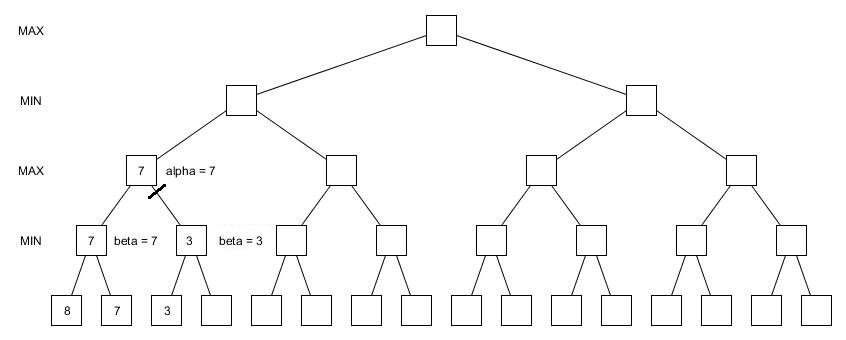
\includegraphics[width = 12 cm]{chapters/minimax/jpg/Alpha-beta3-1.jpg}
\end{center}

Somit erreicht MAX an dem Knoten einen Nutzwert von 7 und der darüber liegende MIN Knoten einen Wert von $<=7$, was bedeutet, dass $\beta = 7$. Betrachten wir nun das nächste Blatt, welches den Nutzwert 9 hat.

\begin{center}
	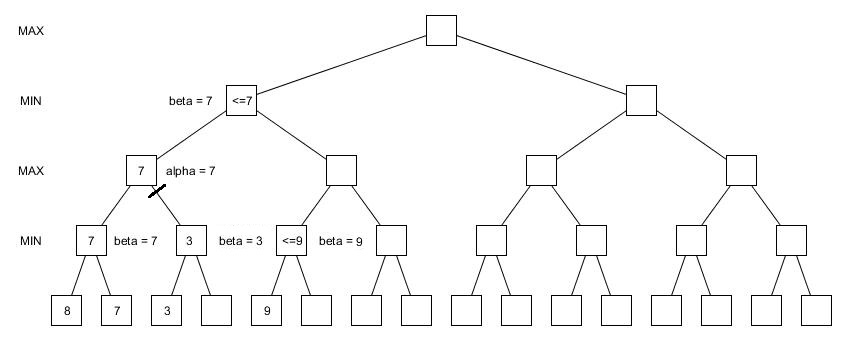
\includegraphics[width = 12 cm]{chapters/minimax/jpg/Alpha-beta4.jpg}
\end{center}

 Da $-\infty = \alpha <9$ müssen wir auch das nächste Blatt betrachten. Anders ausgedrückt, wir können nicht ausschließen das MIN das rechte Blatt wählen würde.

 \begin{center}
 	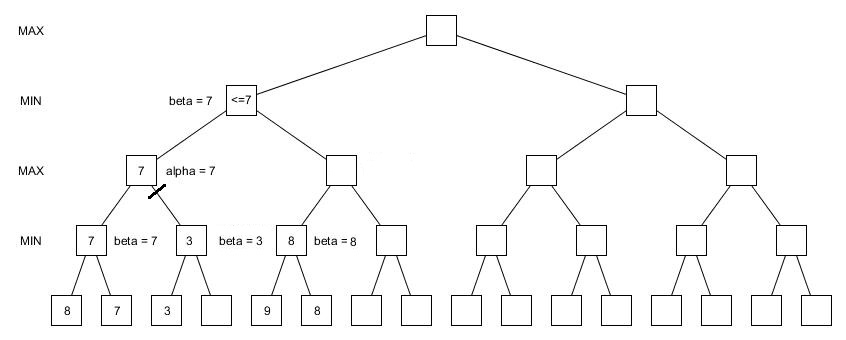
\includegraphics[width = 12 cm]{chapters/minimax/jpg/Alpha-beta5.jpg}
 \end{center}

 Da das nächste Blatt den Nutzwert 8 hat, würde MIN diesen Zug wählen, da sein Nutzwert kleiner ist als der des anderen Zuges ($min\{\beta, 8\}= min\{9,8\}=8$). Somit aktualisiert sich der Wert von $\beta$ auf 8.

 \begin{center}
 	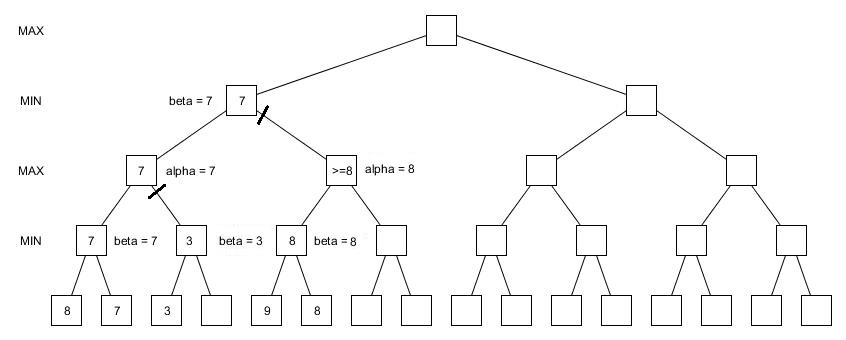
\includegraphics[width = 12 cm]{chapters/minimax/jpg/Alpha-beta6.jpg}
 \end{center}

 Dies hat zur Folge das $\alpha =8$, da MAX im darüber liegenden Zug mindestens einen Nutzwert von 8 erreicht. Somit hat er einen größeren Wert als der linke MAX Knoten, weshalb sich MIN nicht den rechten Knoten aussuchen würde und wir somit auch den Teilbaum nicht weiter betrachten müssen. Anders ausgedrückt, da für den rechten Teilbaum der MAX Knoten einen Wert von mindestens 8 hat und  $\beta = 7$ ist, gilt $\beta<8$ und es findet ein Cutoff statt.  Aufgrund dessen hat der MIN Knoten den Wert 7.

 \begin{center}
 	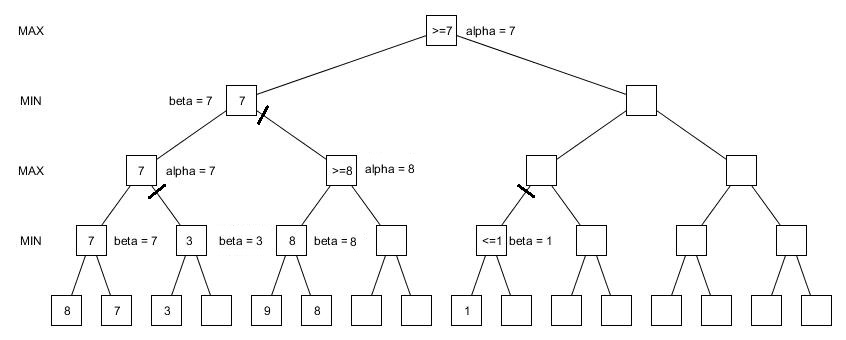
\includegraphics[width = 12 cm]{chapters/minimax/jpg/Alpha-beta7.jpg}
 \end{center}

 Für die Wurzel ergibt sich somit ein Wert von mindestens 7 und $\alpha = 7$
 Die Betrachtung des nächsten Blattes liefert das der MIN Knoten höchstes den Wert 1 hat. Da 1 <$\alpha$ ist eine weitere Betrachtung des Teilbaumes nicht nötig und wir können ihn abschneiden. Mit anderen Worten würde MAX nicht den Zug dieses Teilbaumes wählen, da der Nutzwert des linken Teilbaumes einen höheren Nutzwert hat.

 \begin{center}
 	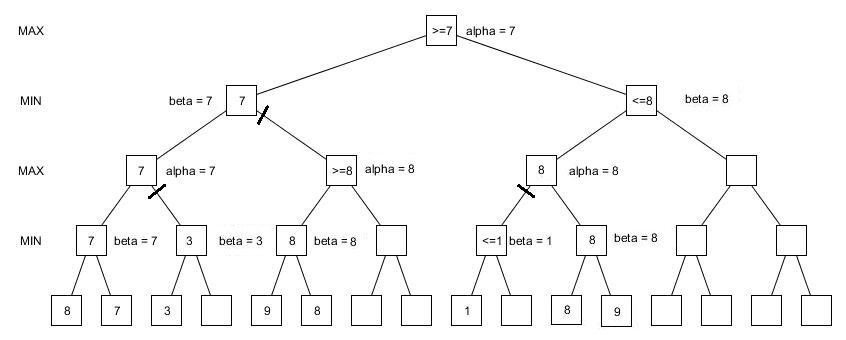
\includegraphics[width = 12 cm]{chapters/minimax/jpg/Alpha-beta8.jpg}
 \end{center}

 Die Auswertung der nächsten beiden Blätter und ihres Elternknotens liefert keine Cutoffs.

 \begin{center}
 	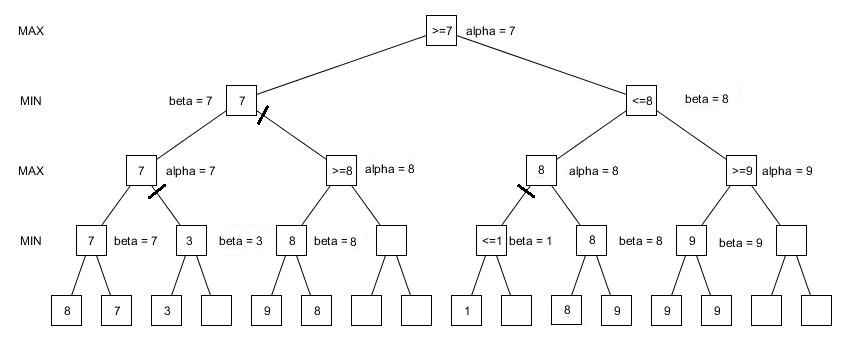
\includegraphics[width = 12 cm]{chapters/minimax/jpg/Alpha-beta9.jpg}
 \end{center}

 Betrachtet man nun die nächsten beiden Blätter liefert das einen Nutzwert von 9 für den MIN Knoten ($\beta =9$) und somit für den MAX Knoten einen Wert $>=9$. Der darüber liegende MIN Knoten würde jedoch nicht den rechten Knoten mit einem Nutzwert $>=9$ wählen, da der linke Knoten nur einen Nutzwert von 8 hat. Somit ist eine weitere Betrachtung des Teilbaumes nicht nötig.\\
 Dies ist somit der endgültige Spielbaum.

 \begin{center}
 	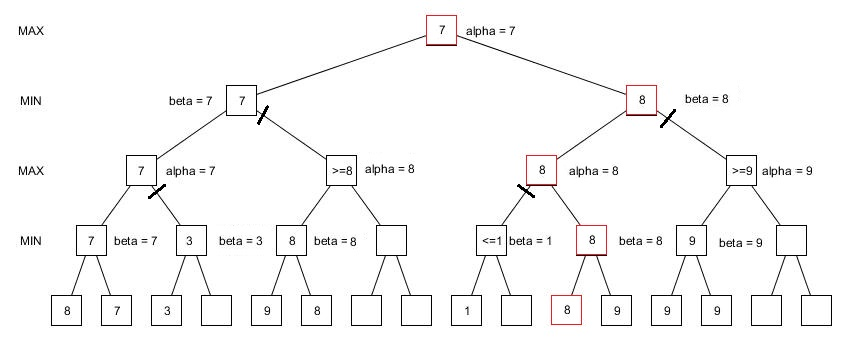
\includegraphics[width = 12 cm]{chapters/minimax/jpg/Alpha-beta10.jpg}
 \end{center}

 Der rot gekennzeichnete Pfad ist der Pfad, der den höchsten Nutzwert liefert, wenn beide Spieler, so wie von uns zu Beginn angenommen, optimal Spielen. Dies bedeutet für den ersten Zug von MAX, dass er den rechten Knoten wählen sollte.

 Für die Berechnung dieses Pfades mussten wir uns 23 Knoten anschauen, wohingegen wir beim Minimax-Algorithmus alle 31 Knoten hätten betrachten müssen, um zu diesem Ergebnis zu gelangen. Somit bietet der Alpha-Beta-Algorithmus in diesem Beispiel eine deutliche Rechenzeitverbesserung.

\section{Abgrenzung / Vergleich zu den vorherigen Kapitel}

In den vorherigen Kapiteln haben wir verschiedene Suchalgorithmen (Bestensuche, Branch-and-Bound, A*) kennengelernt. Diese liefern den Pfad, der zu dem Blatt mit dem höchsten Nutzwert führt. Jedoch beachten sie nicht, ob der Gegner auch diesen Pfad wählen würde. Der Gegner würde versuchen den geringsten Nutzwert für uns zu erreichen und somit versuchen von diesem Pfad abzuweichen.Folglich würden sie keine realistische Einschätzung darüber geben, welche Züge das beste Spielergebnis liefern. Im Gegensatz dazu betrachten sowohl der Minimax, als auch der Alpha-Beta Algorithmus das Verhalten des Gegners, welches zu einer guten Einschätzung der Spielsituation führt.



\section{Fazit \& Bewertung}

Zusammenfassend lässt sich sagen, dass der Minimax- und der Alpha-Beta-Algorithmus zum selben besten Ergebnis für den MAX Spieler führen und sich lediglich in ihrer Effizienz unterscheiden können, da der Alpha-Beta-Algorithmus weniger Berechnungen und somit eine kürzere Rechnungszeit benötigen kann. Je nach Suchbaum kann die Anzahl der Cutoffs und die Einsparung der Rechenzeit sehr groß ausfallen. Aufgrund dessen ist der Alpa-Beta-Algorithmus eine Grundlage für viele Algorithmen im Bereich der Nullsummenspiele für zwei Personen. Für die Berechnungen der Algorithmen sind die Werte der Blätter von größer Bedeutung, welche durch die Heuristik gegeben sind. Alles in allem kann man sagen, dass man sowohl mit Minimax als auch mit Alpha Beta einen Computergegner programmieren kann, der es einem Menschen sehr schwer, wenn nicht sogar unmöglich, macht zu gewinnen und somit eine künstliche Intelligenz bei Nullsummenspielen für die Zukunft denkbar ist.


\section{Quellen und Literatur}

\begin{itemize}
\item MIT - Lecture 6: Search: Games, Minimax, and Alpha-Beta
\item http://home.in.tum.de/~adorf/pub/alphabeta-seminar-paper.pdf
\item https://de.wikipedia.org/wiki/Minimax-Algorithmus
\item https://de.wikipedia.org/wiki/Alpha-Beta-Suche
\end{itemize}


\part{Lernende Systeme}
\chapter{Support-Vector-Machines}
\usetikzlibrary{calc}
\usetikzlibrary{positioning}
\usetikzlibrary{matrix}

\section{Intro \& Motivation}
Obwohl keine allgemein anerkannte Definition von Intelligenz in Menschen (oder
Tieren) existiert, ist durchaus Konsens über wichtige Merkmale intelligenten
Verhaltens gegeben. So gut wie allen Defitionsversuchen ist gemein, dass Intelligenz
mit der Fähigkeit einhergeht, sich in einer sich ändernden Umwelt zurecht zu finden
und der Fähigkeit schnell zu lernen. Im Allgemeinen findet Lernen und die Adaptation
an Umweltgegebenheiten zum Erreichen bestimmter Ziele statt. Legg und Hutter
$($2007$)$ schlussfolgern in ihrer Sammlung verschiedener Definitionsversuche:

\begin{quote}
``Intelligence measures an agent’s ability to achieve goals in a wide range of
  environments. Features such as the ability to learn and adapt, or to understand,
  are implicit in the above definition as these capacities enable an agent to succeed
  in a wide range of environments.''
\end{quote}

Da bestimmte physikalische Prozesse immer chaotisch, das heißt nicht deterministisch
ablaufen, können nicht alle Veränderungen von Umweltbedingungen vorausgessagt
werden. Ein intelligentes System demnach notwendigerweise mit Unsicherheit umgehen
können, um sinnvoll zu handeln $($Lawrence, 2016$)$. Es ist nicht möglich einem
intelligenten System die Voraussetzungen für alle möglichen zukünftigen Entwicklungen
mit auf den Weg zu geben. Wenn es nicht lernen kann, ist es kein intelligentes
System.  Die Fähigkeit sich auf neuartige Umgebungen einzustellen ist also essentiell
für intelligentes Verhalten. Die Voraussetzung für eine solche Anpassung ist eine
sehr allgemeine Fähigkeit aus Erfahrung und Beobachtung zu lernen -- Lernen ist der
Mechanismus, der eine individuelle Adaptation ermöglicht. Eine weitere Voraussetzung
für intelligentes Lernen ist das Vorhandensein eines oder mehrerer Ziele, die
bestimmen aus welchen Informationen überhaupt gelernt werden soll.

Ein intelligentes, anpassungsfähiges System muss also einen Lernmechanismus besitzen,
mit dem das System sich selber verbessern, zeitüberdauernd Ziele verfolgen und den
Erreichungsfortschritt überwachen kann. Dies ist gerade dann relevant, wenn sich
gegebene Umweltbedingungen verändern und Handeln angepasst werden muss. Wenn
beispielsweise ein Computersystem überwachen soll, was für Situationen mit hoher
Wahrscheinlichkeit zu einer Gefährdung des Straßenverkehrs führen, muss das System
etwaige Änderungen in den Rahmenbedingungen -- zum Beispiel technologische
Erneuerungen, Änderungen der gesetzlichen Bestimmungen oder Änderungen des
Verkehrsaufkommens -- in seiner zukünftigen Vorhersage berücksichtigen. Das System
muss durch Lernen aus Beobachtung einschätzen, welchen Gegebenheiten mit dem
Auftreten von Unfällen zusammenhängen, um für die Zukunft Vorhersagen zu erstellen
und gegebenenfalls Interventionsmaßnahmen einzuleiten.

\section{Arten des maschinellen Lernens}
Es gibt verschiedenen Klassifikatoren die dazu genutzt werden um Proben in einem mehrdimensionalen Raum Klassen zuzuordnen.
Dabei kann man Klassifikatoren in drei Arten unterscheiden.
\begin{enumerate}
\item Unüberwachtes Verfahren: Klassen müssen vom Klassifikator erkannt werden.
\item Überwachtes Vefahren: Klassen werden vorher in einer Trainingsphase erlernt.
\item Bestärkendes Verfahren: Klasseneinteilung ist nicht fest und wird durch hinzufügen von Informationen korrigiert.
\end{enumerate}
Dabei gehört die Support Vector Machine zu Art zwei. Zuerst wird eine Trainingsphase durchlaufen anhand der Klassi kator lernt die Klassen zu unterscheiden. Nach der Trainingsphase können neue Daten mit Hilfe eines erstellten Modells zu einer der beiden Klassen zugewiesen werden.

Die folgende Ausarbeitung beschäftigt sich mit den Grundlagen statistischen Lernens,
welches maschinellen Systemen das Lernen aus Beobachtung ermöglicht. Hierbei gehe ich
vor allem auf das sogenannte \emph{überwachte Lernen} ein und beziehe mich in erster
Linie auf die Quellen \emph{Artificial Intelligence -- A Modern Approach} $($3. Ed.,
Kap. 18; Russel \& Norvig, 2010$)$ und \emph{An introduction to Statistical
  Learning} $($James, Witten, Hastie \& Tibshirani, 2013$)$.

\section{Lernen aus Daten}

Damit ein System intelligent lernen kann, müssen Beobachtungen in ein Format gebracht
werden, mit dem das System umgehen kann. Menschen und Tiere besitzen primäre
Sinnesorgane, die Informationen über die Umwelt über Nervenlaufbahnen in ein
zentrales Nervensystem transferieren. Dort werden Informationen aus verschiedenen
Sinnesmodalitäten integriert und Handlungen geplant; vereinfacht gesagt liegen
Informationen in Form von Nervenimpulsen vor. Ein Computersystem muss Informationen
über die Umwelt in einem quantifizierten, numerischen Datenformat erhalten. Auch
Daten, die disktinkte, qualitative Merkmale repräsentieren -- beispielsweise die
Marke eines Autos -- werden dem Computersystem in numerischer Form übergeben.

Beim sogenannten überwachten Lernen (\emph{supervised learning}) werden Daten
allgemein im folgenden Format dargestellt: Betrachtet werden \emph{n} Datenpaare


\begin{equation*}
    (x_{1}, y_{1}), (x_{2},y_{2}), \ldots, (x_{n}, y_{n}).
\end{equation*}

Hierbei bezeichnen $x_{i}$, die \emph{Input} Variablen, $y_{i}$
die \emph{Output} Variablen. $X_{i}$ ist dabei entweder ein einzelner Wert
oder ein Vektor beliebig vieler Werte. Eine Input-Variable könnte beispielsweise die
Geschwindigkeit eines Autos, die Automarke oder das Temperament und Geschlecht des
Autofahrers darstellen. Ziel des überwachten Lernens ist mithilfe der vorhandenen
Input Variablen $($auch genannt: Features, Prädiktoren, unabhängige Variablen$)$
zuverlässige Informationen über den Output (auch genannt: abhängige Variablen,
Labels) zu erlangen.

Die Output Werte y könnten beispielsweise repräsentieren, ob ein
Auto am Tag der Datenaufzeichnung einen Unfall hatte. Dies stellt ein qualitatives
Label dar: die Variable nimmt zwei distinkten Zustände an, entweder \emph{Unfall --
  Ja} oder \emph{Unfall -- Nein} (im Computer dargestellt als 1 / 0). Probleme, in
denen solch ein qualitativer Output vorhergesagt werden soll, werden
\textbf{Klassifikationsprobleme} genannt; existieren genau zwei qualitative
Kategorien, handelt es sich um ein \emph{binäres} Klassifikationsproblem. Angenommen,
das System soll nicht vorhersagen, ob Autos genau am Tag der Aufzeichnung einen
Unfall haben. Schließlich ist für ein einzelnes Auto das Auftreten eines Unfalls sehr
selten und die Variable ist somit wahrscheinlich nicht sehr informativ. Trotzdem soll
das System eine Prognose für die Fahrsicherheit eines jeden beobachteten Autos
ausstellen, damit in Zukunft riskante Verkehrssituationen mit hoher Präzision
eingeschätzt werden können. In diesem Fall könnte als Output die Fahrstrecke, die ein
Auto nach der Aufzeichnung noch unfallfrei fährt, dienen. Die Fahrstrecke stellt eine
kontinuierliche Variable dar -- es werden nicht qualitativ verschiedene Kategorien
betrachtet. Mit der Vorhersage kontinuierlicher Variablenwerte beschäftigen sich die
sogenannten \textbf{Regressionsprobleme}. Tabelle 2.1 zeigt einige exemplarische
Input- und Outputwerte für das Regressionsproblem unseres Fahrsicherheitssystems.

\begin{table}[h!]
  \centering
  \caption{Beispielhafte Input- und Outputwerte für das Fahrsicherheitssystem.}

\vspace{0.3cm}

  \label{tab:svm_table1}
  \def\arraystretch{1.5}%
  \begin{tabular}{l|c|c|c||c|c}
    & Automarke & Geschwindigkeit & Laune & Unfallfreie Fahrstrecke &\\
    \hline
    x\textsubscript{1} & Volvo & 73 km/h & fröhlich & 14,302 km & y\textsubscript{1}\\
    \hline
    x\textsubscript{2} & VW & 144 km/h & neutral & 10,219 km & y\textsubscript{2}\\
    \hline
    x\textsubscript{3} & Audi & 129 km/h & traurig & 21,219 km & y\textsubscript{3}\\
    \hline

    & ... & ... & ... & ... &\\
    \hline
    x\textsubscript{n} & Porsche & 267 km/h & wütend & 22 km & y\textsubscript{n} \\

  \end{tabular}
\end{table}

\vspace{0.3cm}

Beim unüberwachten Lernen (\emph{unsupervised learning}) liegen keine Informationen
bezüglich möglicher Output-Variablen vor -- hier wird alleine in den Input-Variablen
nach Gesetzmäßigkeiten gesucht, um die Daten auf bestimmte Art und Weise zu
strukturieren oder klassifizieren. Dies wäre in unserem Beispiel der Fall, wenn gar
keine Information bezüglich des Auftretens von Unfällen vorliegen würden. Die
vorhandenen Daten könnten trotzdem nach systematischen Regelmäßigkeiten untersucht
werden, etwa mittels \emph{Clustering}. Beispielsweise könnte sich herausstellen,
dass männliche Fahrer in Sportwagen generell jähzorniger sind als weibliche
Fahrerinnen in Kleinwagen -- ohne, dass man dies zuvor explizit erwartet hätte.

Im semi-überwachten Lernen existieren zu manchen Datenpunkte (x\textsubscript{i},
y\textsubscript{i}) Outputwerte y, aber für manche nicht. Dies wäre beispielsweise
der Fall, wenn die Datensammlung nicht lange genug gegangen ist, um für alle
beobachteten Autos die Fahrdistanz bis zum nächsten Unfall zu beobachten.

\subsection{Überwachtes Lernen}

Beim überwachten Lernen wird generell angenommen, dass y durch die Prädiktoren X =
(x\textsubscript{1}, x\textsubscript{2}, ..., x\textsubscript{n}) beschrieben werden
kann. Dabei soll es eine wahre Funktion $f$ geben, die y in Abhängigkeit von X
darstellt:

\begin{equation*}
y = f(X)
\end{equation*}


Ziel des überwachten Lernens ist es eine Funktion \emph{h} zu finden, welche die
wahre Funktion \emph{f} möglichst gut approximiert -- das intelligente System soll
\emph{f} lernen, indem verschiedene Kandidaten-Funktionen untersucht werden. Diese
Form des Lernens wird auch \emph{induktives Lernen} genannt: aus beobachteten
Phänomenen sollen allgemeine Regeln abgeleitet werden, durch die die Beobachtungen
erklärt werden können. Da die wahre Funktion \emph{f} im Allgemeinen unbekannt ist
und nicht bestimmt werden kann, ist man in der Praxis häufig daran interessiert eine
solche Funktion \emph{h} zu bestimmen, die y möglichst fehlerfrei vorhersagt. Zu
diesem Zweck werden die untersuchten Funktionenen an einem Trainingsdatensatz
trainiert und die Vorhersagegüte wird dann an einem unabhängigen Testdatensatz
überprüft. Ziel ist es, den Testdatensatz anhand der Passung, die am
Trainingsdatensatz erstellt wurde, möglichst gut vorherzusagen.  Ob die Funktion
\emph{h} der wahren Funktion \emph{f} ähnelt, ist zumeist gar nicht so wichtig
solange sie akkurate Vorhersagen bezüglich der Zustände der Outputvariablen macht. In
Klassifikationsproblemen kann die Vorhersagegüte einfach durch den prozentualen
Anteil aller falschen Zuordnungen angegeben werden. Im Fall binärer Entscheidungen
kann die Korrektheit von Entscheidungen mit einer 2x2 Tabelle dargestellt werden:

\begin{table}[h!]
  \centering
  \caption{Entscheidungsmöglichkeiten in einer binären Klassifikationsaufgabe.}

\vspace{0.3cm}
  \def\arraystretch{1.5}%
  \label{tab:svm_table2}
  \begin{tabular}{c|c|c}
     & Status: Unfall & Status: kein Unfall \\

 \hline
    \parbox[t]{2.2cm}{Vorhersage:\\ Unfall\\}
    & \parbox[t]{2.2cm}{richtige\\Klassifikation \\}
    & \parbox[t]{2.2cm}{falsche\\Klassifikation \\} \\

 \hline
    \parbox[t]{2.2cm}{Vorhersage:\\ kein Unfall\\}
    & \parbox[t]{2.2cm}{falsche\\Klassifikation \\}
    & \parbox[t]{2.2cm}{richtige\\Klassifikation \\} \\


  \end{tabular}
\end{table}

\vspace{0.3cm}

In Regressionsproblemen ist die einfache Vorhersage-Trefferrate kein sinnvolles
Gütekriterium für die Passung einer Funktion. Angenommen, \emph{h} bestimmt für einen
Fahrer eine unfallfreie Fahrt von 1,237.47 Kilometer, das Auto hat den nächsten
Unfall aber nach 1,237.48 km -- die Vorhersage liegt sehr nah am tatsächlichen Wert,
ist aber nicht korrekt. Ist diese Abweichung als problematisch zu betrachten?  Wäre
eine Vorhersage von 20,000 km ``gleich falsch''? Es macht Sinn in diesem Fall den
Schweregrad der Abweichung der Vorhersage zu berücksichtigen. Bei kontinuierlichem
Output wird deswegen der Vorhersagefehler durch die Abweichungen der vorhergesagten
von den tatsächlichen y-Werten bestimmt. Dabei wird häufig die mittlere quadratische
Abweichung (\emph{mean squared error}; MSE) als Fehlermaß verwendet.

\vspace{0.3cm}

$MSE=\displaystyle \frac{1}{n} \displaystyle \sum_{i=1}^{n} (y_i - h(x_i))^2$

\vspace{0.3cm}

Hierbei sind y\textsubscript{i} die beobachteten Output-Werte und
\emph{h}(x\textsubscript{i}) die vorhergesagten Werte auf Basis der zugehörigen
Input-Werte.

Die Funktion \emph{h} sollte sollte so gewählt werden, dass die Vorhersagefehler
gering gehalten werden. Tatsächlich wird aber bei der Wahl von \emph{h} nicht nur die
Fehlerrate minimiert, sondern die \textbf{Kosten} verschiedener Fehlentscheidungen
können ebenfalls berücksichtigt werden. Nicht alle Fehleinschätzungen sind gleich
problematisch: eine starke Unterschätzung der verbleibenden unfallfreien Zeit wäre
beispielsweise fataler als eine Überschätzung, da im ersteren Fall mögliche
Interventionsmaßnahmen zu spät ergriffen würden. Im binären Fall wäre analog die
falsche Vorhersage schlimmer, dass kein Unfall stattfindet, obwohl ein Unfall
stattfinden wird (siehe die zwei Fehlertypen in Tabelle 2.2). Demnach muss ein
solches \emph{h} gesucht werden, welches einerseits gute Vorhersagen erlaubt, und
andererseits die Kosten möglicher Fehler minimiert.

Wie aber wird bestimmt, welche Funktionen \emph{h} untersucht werden als Schätzer für
\emph{f}? Der Hypothesenraum \emph{H} definiert, welche Funktionen als Kandidaten für
\emph{f} untersucht werden. Ein Lernproblem wird realisierbar genannt, wenn \emph{H}
die wahre Funktion \emph{f} enthält. Der Hypothesenraum \emph{H} wird nach Funktionen
durchsucht, die gut mit den Daten übereinstimmen. Eine Hypothese (d.h. eine
hypothetisierte Funktion) heißt konsistent, wenn sie alle Trainingsdaten korrekt
beschreibt. Sie heißt generalisierbar, wenn sie auch für Testdaten eine gute
Vorhersage erlaubt. Man kann sinnvollerweise annehmen, dass ernsthaft falsche
Hypothesen bereits nach der Beobachtung von nur wenigen Datenpunkten stark von der
Realität abweichende Vorhersagen machen, sodass diese schnell ausgeschlossen werden
können.

\subsection{Lineare Regression}

Im Falle einer Regressionsentscheidung könnte der Hypothesenraum aus der Klasse der
linearen Polynome bestehen, das heißt Funktionen der Form:

\begin{equation*}
y = \beta_0 + \beta_1 x_1 + \beta_2 x_2 + ... + \beta_n x_n
\end{equation*}

Hier wird der Output \emph{y} durch eine Linearkombination der Inputvariablen
x\textsubscript{i} dargestellt. $\beta \textsubscript{i}$ sind Koeffizienten, die so
gewählt werden, dass die quadratische Abweichung der vorhergesagten Daten \emph{y}
von den tatsächlichen Daten möglichst wenig abweicht. Dieses Verfahren wird
\textbf{Methode der kleinsten Quadrate} genannt. Man kann zeigen, dass die
Minimierung der quadratischen Abweichungen zu einer eindeutigen Lösung der
Koeffizienten $\beta \textsubscript{i}$ führt. Für die Datenmatrix $X = [1, x_1, x_2,
  .., x_n]$, wobei $x_i$ ein Vektor ist, der die Werte der i'ten Prädiktorvariablen
darstellt, und $\beta = [\beta_0, \beta_1, \beta_2, ..., \beta_n]$, ist diese Lösung
gegeben durch

\begin{equation*}
\beta = (X^TX)^{-1}X^Ty
\end{equation*}

Für Menschen sind lineare Zusammenhänge gut zu verstehen und mathematisch sowie von
der Rechenintesität einfach durchzuführen. Lineare Zusammenhänge können in der Weise
``Wenn Variable \emph{x} steigt, steigt / sinkt Variable \emph{y}'' interpretiert
werden. Komplexere, nicht-lineare Verfahren wie Support-Vektor-Maschinen und
Neuronale Netze schneiden in ihrer Vorhersagegüte häufig besser ab als einfache
lineare Regression, sind aber rechenintensiver und für Menschen weniger leicht
interpretierbar. Dies ist für ein weit entwickeltes intelligentes Computersystem aber
gegebenenfalls kein Problem mehr -- sofern Menschen dem Urteilvermögen des Systems
vertrauen.

Wir könnten die Hypothese aufstellen, dass zwischen der beobachteten Geschwindigkeit
eines Autos und der zu erwartenden unfallfreien Fahrstrecke ein negativer linearer
Zusammenhang besteht -- schnellere Fahrer könnten nach weniger gefahrenen Kilometern
einen Unfall bauen. Dies ist ein Fall von \textbf{univariater Regression}: der Output
wird vorhergesagt durch nur eine Prädiktor-Variable. Grafik 2.1 stellt einen
möglichen Zusammenhang der beiden Variablen dar.

\begin{figure}[!ht]
  \caption{Ein linearer Zusammenhang zwischen Geschwindigkeit und der Länge der
    Strecke einer weiteren unfallfreien Fahrt.}  \centering
  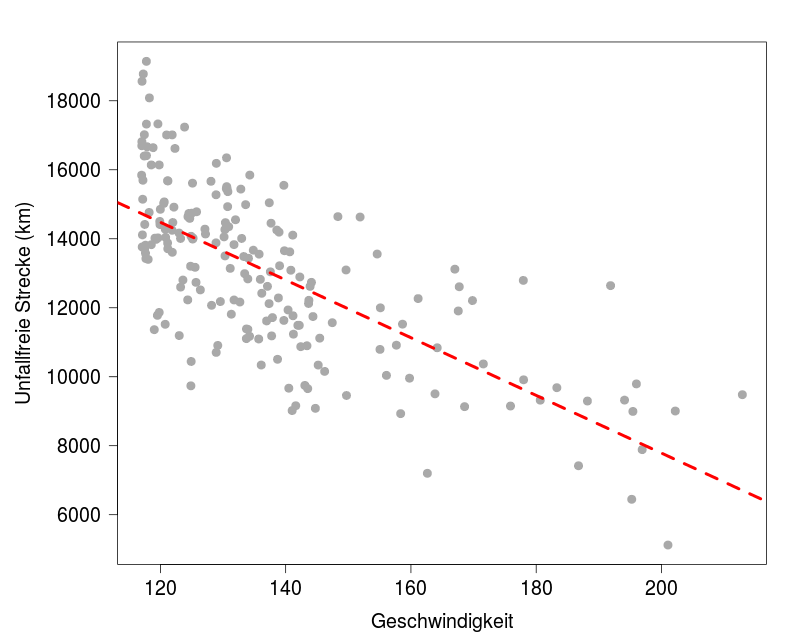
\includegraphics[width=1\textwidth]{chapters/svm/plot_lds.png}
\end{figure}

Es zeigt sich, dass schnelle Autofahrer tendentiell bereits nach einer kürzeren
Strecke einen Unfall haben. Die rote Gerade zeigt hierbei die vorhergesagten
Distanzwerte an, die allein durch Kenntniss der Variable Geschwindigkeit zu erwarten
sind. Die Gerade wird beschrieben durch die Gleichung:

\begin{equation*}
y = 24,516.56 - 83.65 * Geschwindigkeit
\end{equation*}

Das lineare Modell sagt somit pro 1 km/h schnelleres Fahren etwa 84 weniger
unfallfrei gefahrene Kilometer vorher. Es ist jedoch deutlich zu erkennen, dass
allein das Wissen über die Geschwindigkeit keine allzu präzise Aussage über die
unfallfreie Strecke ermöglicht -- im Mittel liegt im vorliegenden Fall die absolute
Abweichung zwischen vorhergesagten und tatsächlichen Werten bei 1401 km. Ein
intelligentes System sollte bessere Prognosen erstellen, wenn seine Aufgabe die
Überwachung der Verkehrsicherheit ist! Um die Vorhersagegüte zu erhöhen, bieten sich
zwei Möglichkeiten an: Erstens können wir mehr aussagekräftige Prädiktoren in unser
Regressionsmodell aufnehmen. In diesem Fall würden wir das Modell zu einem
\textbf{multivariaten Regressionsmodell} erweitern.x Zweitens könnten wir die
Komplexität der Modellgleichung erweitern, um auch nicht-lineare Schwankungen in den
Daten zu beschreiben.

\subsection{Nicht-lineare Regression}

Lineare Regressionsverfahren können erweitert werden, um auch nicht-lineare
Zusammenhänge zu beschreiben. Somit ergibt sich eine höhere Flexibilität,
Schwankungen in Daten abzubilden. Um nicht-lineare Zusammenänge mithilfe der
\emph{linearen} Regression zu beschreiben, wird die Modellgleichung als Polynom
höherer Ordnung aufgestellt. Dabei bleibt die Gleichung linear in den Koeffizienten,
jedoch die Prädiktorvariablen gehen mit bis zu d-wertigen Polynomgrad in das
Regressionsmodell ein. Für ein Polynom d-wertiger Ordnung mit einer
Prädiktorvariablen \emph{x} sieht in die Regressionsgleichung somit wie folgt aus:

\begin{equation*}
y = \beta_0 + \beta_1 x + \beta_2 x^2 + ... + \beta_d x^d
\end{equation*}

Die allgemeine Koeffizientenlösung gilt auch für höherwertige Polynome, wobei in
diesem Fall für die Datenmatrix gilt X = $[1, x, x^2, ..., x^d]$, mit $\beta =
[\beta_0, \beta_1, \beta_2, ..., \beta_d]$:

\begin{equation*}
\beta = (X^TX)^{-1}X^Ty
\end{equation*}

Angenommen unser System möchte seine Verhersagegenauigkeit verbessern und betrachtet
weitere Variablen, die mit dem Auftreten von Verkehrsunfällen auftreten können. Es
stellt fest, dass das die Häufigkeit von Auffällen mit der Tageszeit zusammenhängt
(siehe Grafik 2.2).


\begin{figure}[!ht]
  \caption{Der Zusammenhang zwischen Uhrzeit und der Häufigkeit von Autounfällen pro
    Jahr.  Die rote Linie stellt den Schätzer der Unfallhäufigkeit durch eine
    einfache lineare Regression dar. }  \centering
  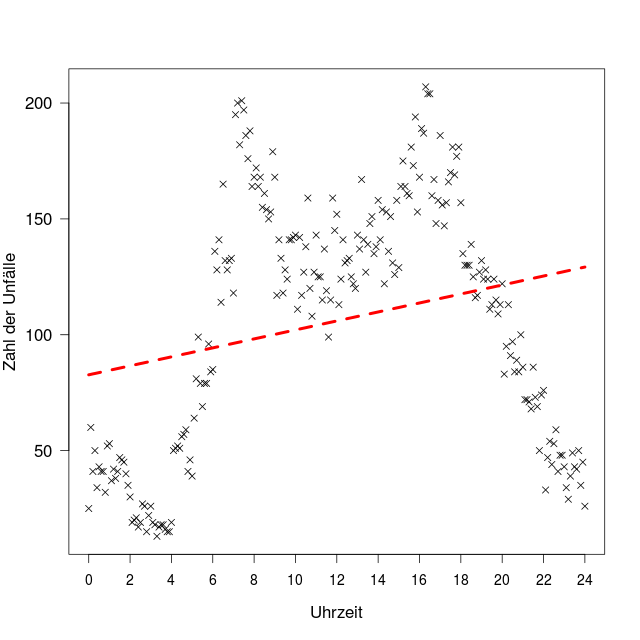
\includegraphics[width=1\textwidth]{chapters/svm/poly_1.png}
\end{figure}


Ein einfaches lineares Regressionsmodell ergibt einen geringen positiven Zusammenhang
zwischen Tageszeit und Zahl der Unfälle. Das Modell sagt somit die größte
Unfallwahrscheinlichkeit für 23:59 Uhr vorher und die geringste für 00:00 Uhr, was
eine sehr unplausibele Vorhersage ist. Eine visuelle Inspektion der Daten ergibt
schnell, dass dieser einfache lineare Zusammenhang die Daten nicht adäquat
beschreibt. Eine Systematik in den Daten geht augenscheinlich darauf zurück, dass
sich nachts weniger Unfälle ereignen als tagsüber. Außerdem scheinen sich tagsüber
während der Zeit des Berufsverkehrs noch einmal etwas mehr Unfälle zu ereignen. Ein
Polynom zweiter Ordnung ist bereits in der Lage den U-förmigen Zusammenhang zwischen
Tageszeit und Unfällen darzustellen, der durch die Reduktion der Unfälle nachts
bedingt wird. Ein Polynom des 10. oder 20. Grades kann die Schwankungen abzubilden,
die auf den Berufsverkehr zurückgehen (siehe Grafik 2.3).

\begin{figure}[!ht]
  \caption{Der Zusammenhang zwischen Uhrzeit und der Häufigkeit von Autounfällen pro
    Jahr.  d ist der Grad der Polynomgleichung, die zur Vorhersage der
    Unfallhäufigkeit verwendet ist.}  \centering
  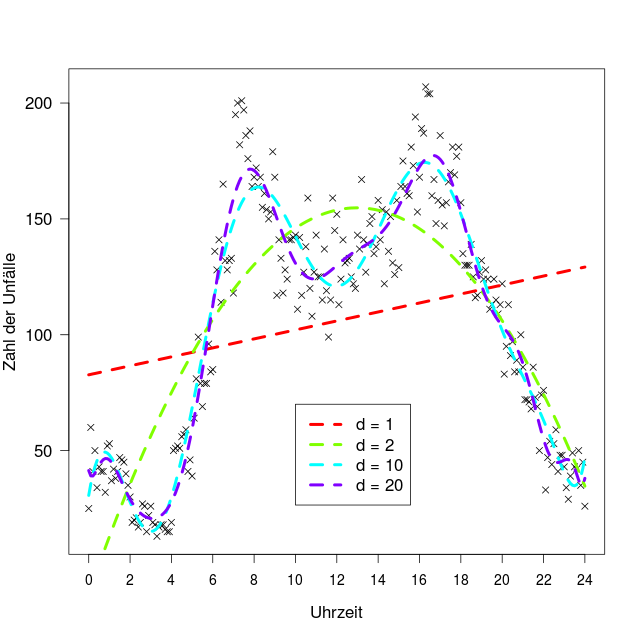
\includegraphics[width=1\textwidth]{chapters/svm/poly_2.png}
\end{figure}


Ist also anzunehmen, dass komplexere Modelle besser sind, da sie Daten genauer
beschreiben können und bessere Vorhersagen treffen? Sollte man in einer polynomialen
Regression immer anstreben den höchst-möglichen Polynomgrad zu modellieren, um die
Daten möglichst präzise abzubilden? Es gibt mehrere Gründe, die dagegen sprechen:
erstens ist nicht zu erwarten, dass jegliche Erweiterung in der Komplexität auch
wirklich zu einer merklich verbesserten Vorhersageleistung führt. In dem Fall besagt
das philosophische Prinzip \emph{Ockhams Razor}, dass wenn verschiedene Hypothesen
Daten gleich gut beschreiben, diejenige gewählt werden sollte mit, welche die
wenigsten Annahmen macht.  Ockhams Razor ist ein allgemeines Prinzip, welches nicht
nur in Regressionsproblemen Anwendung findet. In Grafik 2.3 ist zu erkennnen, dass
ein Polynom 2. Grades die Daten schon wesentlich besser abbildet als der einfach
lineare Zusammenhang. Das Polynom 10. Grad ist wiederum ebenfalls eine Verbesserung,
da es Schwankungen, die auf den Berufsverkehr zurückgehen, abbildet. Es ist jedoch
fraglich, ob die Erhöhung der Komplexität von 10 auf 20 Polynomgrade wirklich
notwendig ist, um die Daten adäquat abzubilden. Nach Ockhams Razor wäre in dem Fall
das weniger komplexe Modell zu bevorzugen.

Desweiteren besteht bei der Annahme eines zu komplexen Modells die Gefahr des
sogenannten \textbf{Overfittings}. Dieses bezeichnet den Umstand, wenn ein Modell
zwar vorgegebene Daten sehr gut beschreibt, aber nicht auf neue Testdaten
generalisiert, d.h. für solche Daten schlechte Vorhersagen macht, die nicht verwendet
wurden, um das Modell zu trainieren. Es ist wichtig, dass ein Modell auch für neue
Datenpunkte Aussagen treffen kann. Für unser Fahrsicherheitssystem wäre es fatal,
wenn es zwar alte Unfalldaten gut rekonstruieren kann, aber nicht zukünfige
Unfallgefahren voraussagen kann -- in dem Fall wäre es sogar vollends unnötig dieses
System überhaupt zu unterhalten.

Um bei der Erstellung eines Modells nicht auf Daten warten zu müssen, die erst in der
Zukunft (oder vielleicht niemals) gesammelt werden können, kann man eine sogenannte
\textbf{Kreuzvalidierung} durchführen: das vorhandene Datenset wird aufgeteilt in
einen \textbf{Trainings-} und einen \textbf{Testdatensatz}. Dies geschieht meistens,
indem ein bestimmter Prozentsatz der Daten zufällig dem Trainigsset und die anderem
dem Testset zugeteilt werden; eine Aufteilung von 80\% zu 20\% ist zum Beispiel
üblich. Anhand der Trainingsdaten werden die Regressionskoeffizieten geschätzt,
entscheidend für die Beurteilung eines Modells ist aber seine Fähigkeit die Testdaten
abzubilden. Dies ist ein allgemeines Prinzip, welches nicht nur bei linearer
Regression Anwendung findet. Im Falle einer Regression werden die Koeffizienten so
gewählt, dass sie den Trainingsdatensatz mit maximal präzise beschreiben. Durch
Annahme höherer Polynomgrade wird die Passung an den Trainingsdatensatz verbessert,
im Testdatensatz verschlechtert sich die Passung jedoch ab einem bestimmten
Komplexitätsgrad: ab hier geschieht Overfitting. Grafik 2.4 zeigt für den Uhrzeit --
Unfallhäufigkeit Datensatz die Modellpassung verschiedener Polynomgrade anhand einer
Kreuzvalidierung. Es zeigt sich, dass Trainingsdaten mit steigendem Polynomgrad
besser vorhergesagt werden. Im Testdatensatz ist bei sehr hoher Komplexität jedoch
wieder eine Verschlechterung der Passung zu sehen. Beachtlich ist hierbei (sowohl für
Trainings- als auch Testdatensatz) die Verbesserung, die erzielt wird, wenn der
Polynomgrad von 1 auf 2 erhöht wird.

\begin{figure}[!ht]
  \caption{Das Ergebnis einer Kreuzvalidierung des Uhrzeit -- Unfallhäufigkeit
           Datensatzes. Gezeigt ist der Verlauf des mittleren Voraussagefehlers nach Komplexität
           des modellierten Polynoms für Trainings- und Testdatensatz.}  \centering
  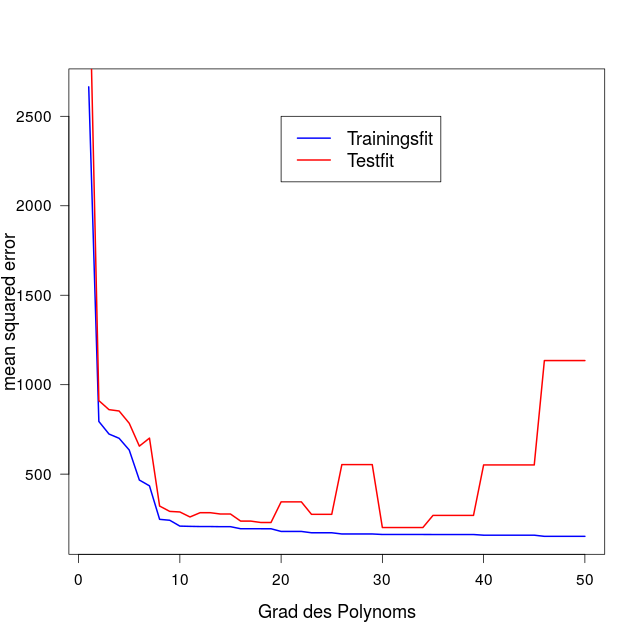
\includegraphics[width=1\textwidth]{chapters/svm/test_training.png}
\end{figure}

\subsection{Klassifikation}

Sehr häufig müssen in der Praxis qualitative Outcome Variablen vorhergesagt
werden. Unser Fahrsicherheitssystem könnte beispielsweise der sehr relevanten Frage
nachgehen, unter welchen Umständen Verkehrsunfälle tödlich ausgehen. Beispielsweise
könnte es betrachten, ob durch Kenntniss des Gewichts und der Geschwindigkeit eines
Autos vorausgesagt werden kann, ob ein Unfall tödlich ausgeht. Grafik 2.5 zeigt für
100 verschiedene in Unfälle involvierte Autos das Gewicht und die Geschwindigkeit,
und ob der Unfall tödlich verlaufen ist. Es zeigt sich, dass eine höhere
Geschwindigkeit tendentiell mit tödlichem Ausgang einhergeht. Zu einem geringeren
Maße hängt auch das Gewicht mit der Tödlichkeit des Ausgang zusammen. Ziel einer
Klassifikation ist eine Funktion zu finden, die auf Basis der Input-Werte das Label
schätzen kann. Hierbei wird eine Entscheidungsgrenze (``decision boundary'')
angewendet; wenn der vorhergesagte Funktionswert über dieser Grenze liegt, wird eine
Klasse vorhergesagt, andernfalls wird die andere Klasse vorhergesagt. Wenn es möglich
ist die Klassen durch eine lineare Gleichung eindeutig voneinander zu trennen -- wie
in Grafik 2.5 der Fall -- nennt man das Problem \textbf{linear separabel}.
Verfahren, die zur Lösung von Klassifikationsproblemen verwendet werden, sind unter
anderem k nearest neighbor, lineare Diskriminanz Analyse, logistische Regression
Support Vector Machines oder neuronale Netze. Dabei können Support Vector Machines
und neuronale Netze sogar nicht-lineare Entscheidungsgrenzen abbilden.

\begin{figure}[!ht]
  \caption{Die Klassifikation eines Autounfalls als tödlich oder nicht tödlich in
    Abhängigkeit des Gewichts und der Geschwindigkeit des Autos. Die blaue Gerade ist
    eine sogenannte Entscheidungsgrenze (``decision boundary'').} \centering
  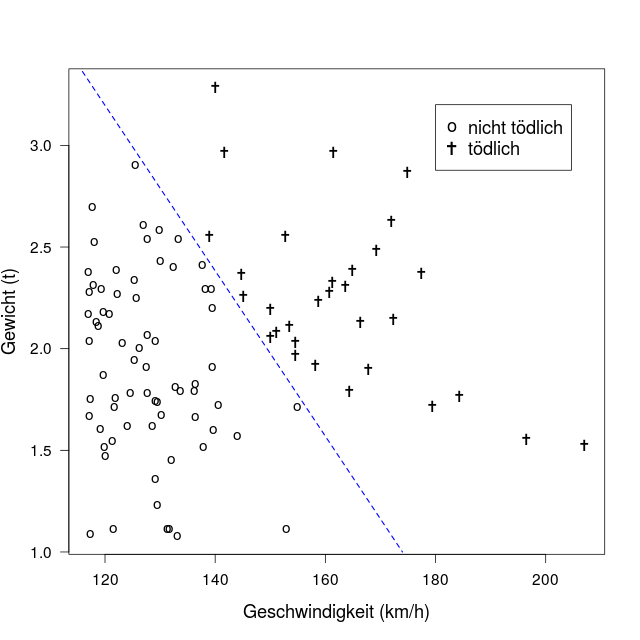
\includegraphics[width=1\textwidth]{chapters/svm/death_data.png}
\end{figure}

\section{Fazit \& Bewertung}

Methoden des statistischen Lernens können verwendet werden, um Computersystemen das
Lernen aus Beobachtungen zu ermöglichen. Die Fähigkeit zu lernen ist eine notwendige
Voraussetzung für maschinelle Systeme intelligentes Verhalten zu zeigen. Systeme
können aus großen Datenmengen Informationen integrieren, um zukünftige Ereignisse
oder Verhalten vorherzusagen. Maschinelles Lernen handelt sich um ein stark
wachsendes Forschungsfeld, das auch in der Öffentlichkeit mit viel Interesse verfolgt
wird -- nicht zuletzt aufgrund kürzlicher, medienwirksamer Errungenschaften
intelligenter Systeme, beispielsweise dem Erfolg des Systems AlphaGo, welches den
Weltmeister Lee Sedol im Go-Spiel überraschend bezwang. Lineare Regression wurde als
wichtiger Prototyp des statistischen Lernens ausführlicher vorgestellt. Dabei handelt
es sich um ein einfaches Verfahren, welches bereits gute Voraussagen liefert und auch
nicht-lineare Zusammenhänge darstellen kann. Auf fortgeschrittenere
Klassifikationsverfahren wie Support Vector Machines und neuronale Netze wurde ein
Ausblick gegeben. Einige grundsätzliche Prinzipien wie Ockams Razor und
Kreuzvalidierung gelten für jegliche Verfahren des statistischen Lernens, egal wie
komplex oder einfach sie erlernt werden können.

\section{Quellen und Literatur}
\begin{itemize}
\item James, G., Witten, D., Hastie, T., \& Tibshirani, R. (2013). \emph{An introduction to
statistical learning}. New York: Springer.

\item Legg, S., \& Hutter, M. (2007). A collection of definitions of intelligence. \emph{Frontiers
in Artificial Intelligence and applications}, 157, 17.

\item Lawrence N. (2016, May 09). Future of AI 6. Discussion of ``Superintelligence: Paths,
Dangers, Strategies'' [Web log post]. Retrieved from \newline
http://inverseprobability.com/2016/05/09/machine-learning-futures-6

\item Russell, S., \& Norvig, P. (2010) \emph{Artificial Intelligence: A modern approach
  (3rd. ed.)}. Upper Saddle River: Pearson.
\end{itemize}

\usetikzlibrary{calc}
\usetikzlibrary{positioning}
\usetikzlibrary{matrix}

\pgfdeclarelayer{background}
\pgfsetlayers{background,main}

\chapterimage{chapter_head_1.png}
\chapter{Neuronale Netze}
\section{Intro \& Motivation}

Heutzutage sind die Rechner so schnell und die Algorithmen so effizient, dass unsere Computer in der Lage sind, die kompliziertesten Berechnungen innerhalb von ein paar Millisekunden durchzuführen. Und jedoch scheitern sie, wenn es um so triviale Aufgaben wie zum Beispiel die Gesichts- oder Stimmerkennung  geht. Für einen Menschen ist es aber gar kein Problem die Gesichter, sogar unter erschwerten Bedingungen (zu dunkel, zu nebelig, usw.), zu erkennen.

Woran kann das liegen? Warum ist es für einen Computer so einfach komplexe Mehrteilchensysteme zu berechnen und wiederum so schwer, auf einem unscharfen Bild ein paar Gesichter zu erkennen, obwohl diese Aufgabe sogar für ein kleines Kind keine Herausforderung ist?

Die Antwort auf diese Fragen ist ganz einfach: Solche Aufgaben (sowie viele andere) hängen von einer Menge Faktoren ab, wie zum Beispiel die Bild- oder Aufnahmequalität, und es ist leider unmöglich einen Algorithmus zu entwickeln, der alle Details berücksichtigt. Zusätzlich ist das menschliche Gehirn im Vergleich zu den Rechnern
nicht nur in der Lage die Informationen zu empfangen und sie zu speichern, wie das die Rechner tun, sondern auch diese Daten gleichzeitig zu verarbeiten, zu analysieren und aus dieser Analyse zu lernen. Deswegen, bevor man versucht dieses Problem zu lösen, muss man sich zuerst fragen, wie es unserem Gehirn gelingt, solche Aufgaben zu bewältigen.

Dabei sollte man auch erwähnen, dass unser Gehirn fast sein komplettes Potenzial ausnutzt, indem es ständig und parallel arbeitet. Es ist bekannt, dass es fast unmöglich ist, die echte Parallelität zwischen den Prozessen in einem Computer zu erreichen. Und das ist noch ein Grund, zu fragen, nach welchen Prinzipien unser Gehirn funktioniert und wie es die Informationen verarbeitet.

\section{Inhaltliche Ausarbeitung des Themas}

\subsection{Zurück in die Vergangenheit}

 Die ersten Schritte in diesem Gebiet haben Warren McCulloch und Walter Pitts gemacht, indem sie im Jahr 1943 „A logical calculus of the ideas immanent in nervous activity“ veröffentlicht haben. In diesem Werk  untersuchen die Wissenschaftler die Fähigkeiten Neuronaler Netze und präsentieren einen einfachen durch Neuronen nachgebauten Schwellwertschalter, der in der Lage ist, fast jede logische und arithmetische Funktion zu berechnen.

Im Jahr 1947 wurde von Walter Pitts und Warren McCulloch vorgeschlagen, dass Neuronale Netze zur räumlichen Mustererkennung eingesetzt werden könnten.

Ein wichtiger Schritt wurde im Jahr 1949 von Donald Olding Hebb gemacht. In seinem Werk „The Organization of Behaviour“ formulierte er die klassische Hebb'sche Lernregel, welche in ihrer allgemeinen Form die Basis fast aller neuronalen Lernvervahren darstellt.

Weitere neuropsychologische Arbeiten erschufen den Weg für spätere erfolgreiche Forschungen in diesem Gebiet.

\subsection{Problemstellung}

Neuronale Netze basieren auf der Ähnlichkeit zu den menschlichen Neuronennetzen. Damit ein Verständnis über den Aufbau und die Funktion der neuronalen Netze erreicht werden kann, muss die Funktionsweise der echten Neuronen verstanden sein.

\subsubsection{Biologische Grundlagen}

Unser Gehirn besteht größtenteils aus Nervenzellen, die auch Neuronen genannt werden. Eine typische Nervenzelle eines Säugetiers besteht hauptsächlich aus drei wichtigen Teilen (siehe Abb. 2.1): dem Zellkörper (Soma) mit Zellkern, dem Axon (Nervenfaser) mit Synapsen und den Dendriten (Zelleingängen).

\begin{figure}[h]
\centering
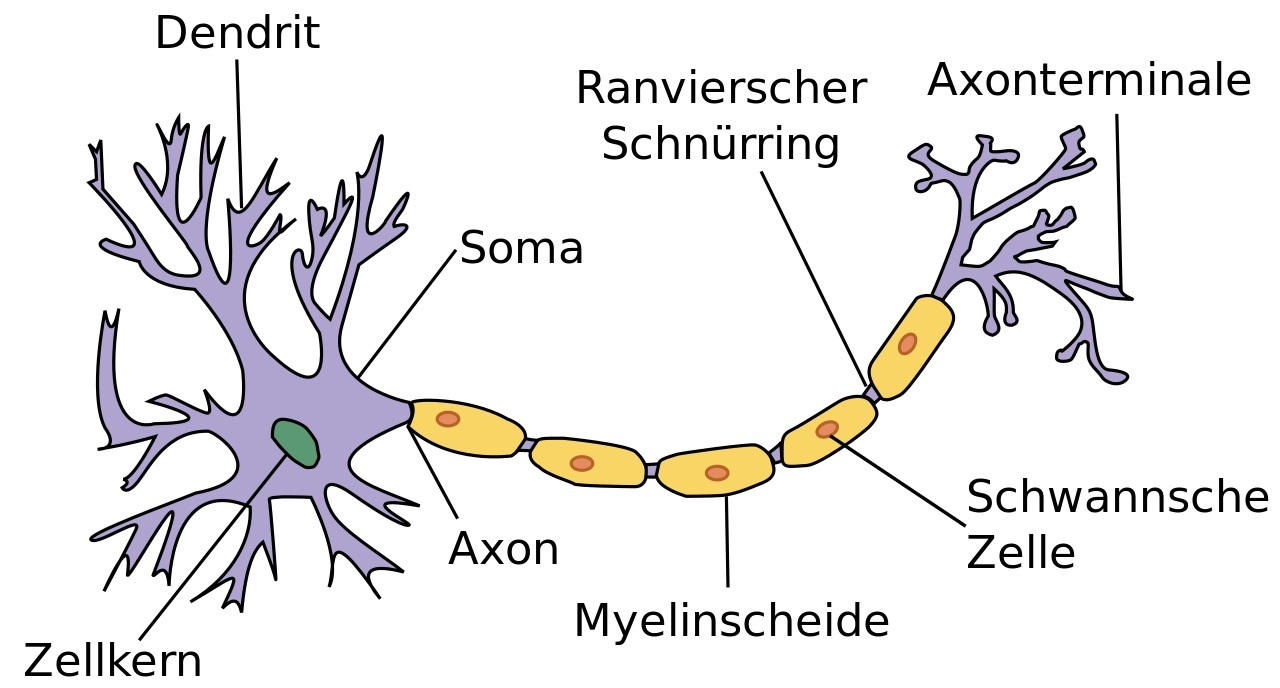
\includegraphics[width=8cm]{chapters/neural_networks/neuron.jpg}

\caption{Schematischer Aufbau eines Neurons (Quelle: Wikipedia)}
	\label{img:neuron}

\end{figure}
Dendriten sind baumartige Eingänge der Nervenzelle und dienen der Aufnahme elektrischer Reize von anderen Nervenzellen und ihrer Übertragung in den Zellkern. Aufgrund ihrer Form werden mehrere Dendriten auch als Dendritenbaum bezeichnet. Die Länge der Dendriten beeinflusst die Stärke des ausgelösten Signals: je kürze ist ein Dendrit, desto stärker ist das Signal. Diese Signale werden an den Zellkörper geleitet, wo sie sich aufsummieren.

Das Axon einer Nervenzelle kann man als „Ausgang“ des Neurons bezeichnen, weil es elektrische Signale weiterleitet, die durch Ladungsunterschiede (elektrischen Potential) zwischen der Umgebung und Zellinnerem entstehen. Wenn das aufsummierte Erregungspotenzial eine bestimmte Schwelle übersteigt, wird ein Aktionspotential fester Stärke ausgelöst, dass über das Axon und den Dendriten weitergeleitet wird.

Am Ende des Axons befinden sich die Verdickungen, die auch Synapsen genannt werden (siehe Abb. 2.2). Synapsen sind mit den Dendriten anderer Neuronen verbunden. Wobei es keine direkte physikalische Verbindung, sondern einen mit Flüssigkeit gefüllten Zwischenraum gibt. Erreicht ein über dem Schwellenwert liegendes Aktionspotential die Synapse, werden sogenannte Neurotransmitter ausgeschüttet. Diese Neurotransmitter wandern durch den synaptischen Spalt und erreichen die Rezeptoren des Dendriten. Die Neurotransmitter können an den Rezeptoren binden. Entweder führt das Anbinden der Neurotransmitter zu einer Reizweiterleitung bzw. Reizverstärkung in den Dendriten oder zu einer Hemmung des Aktionspotentials, sodass die Reizweiterleitung zum Erliegen kommt.  Die durchschnittliche Anzahl an solchen Verknüpfungen beträgt ca. 14 000 pro Neuron.

\begin{figure}[h]
\centering
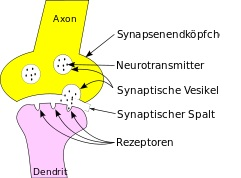
\includegraphics[width=4cm]{chapters/neural_networks/synapsen.jpg}

\caption{Synapsenkommunikation (Quelle: Wikipedia)}
	\label{img:synapsen}

\end{figure}

Der Zellkörper ist der Hauptbestandteil eines Neurons. Er ist nicht nur für die Energieproduktion verantwortlich, sondern auch für die Verarbeitung und Aufsummierung der eingehenden Signale sowie der Erzeugung bzw. Weiterleiitung der Ausgangssignale.

Die neurologischen Kenntnisse über den Aufbau menschliches Gehirns bilden die Basis für die Entwicklung mathematischer Modelle, die auch „Neuronale Netze“ genannt werden.



\section{Aufbau und Funktionsweise künstlicher  Neuronaler Netze (KNN)}


Jedes künstliche neuronale Netz hat drei Grundelemente: Neuronen, die Verbindungen zwischen den Neuronen und Lernregeln.

\subsection{Neuronen}

Ähnlich den Nervenzellen im menschlichen Gehirn sind die künstlichen „Neuronen“ die wichtigsten Bestandteile eines KNNs. Sie besitzen eine ähnliche Struktur mit vielen Ein- und Ausgängen für die Weiterleitung von ein- und ausgehenden Signalen sowie einen Körper zur Verarbeitung dieser Signale. Schematisch könnte ein künstliches Neuron folgendermaßen aussehen (siehe Abb. 3.1):

\begin{figure}[h]
\centering
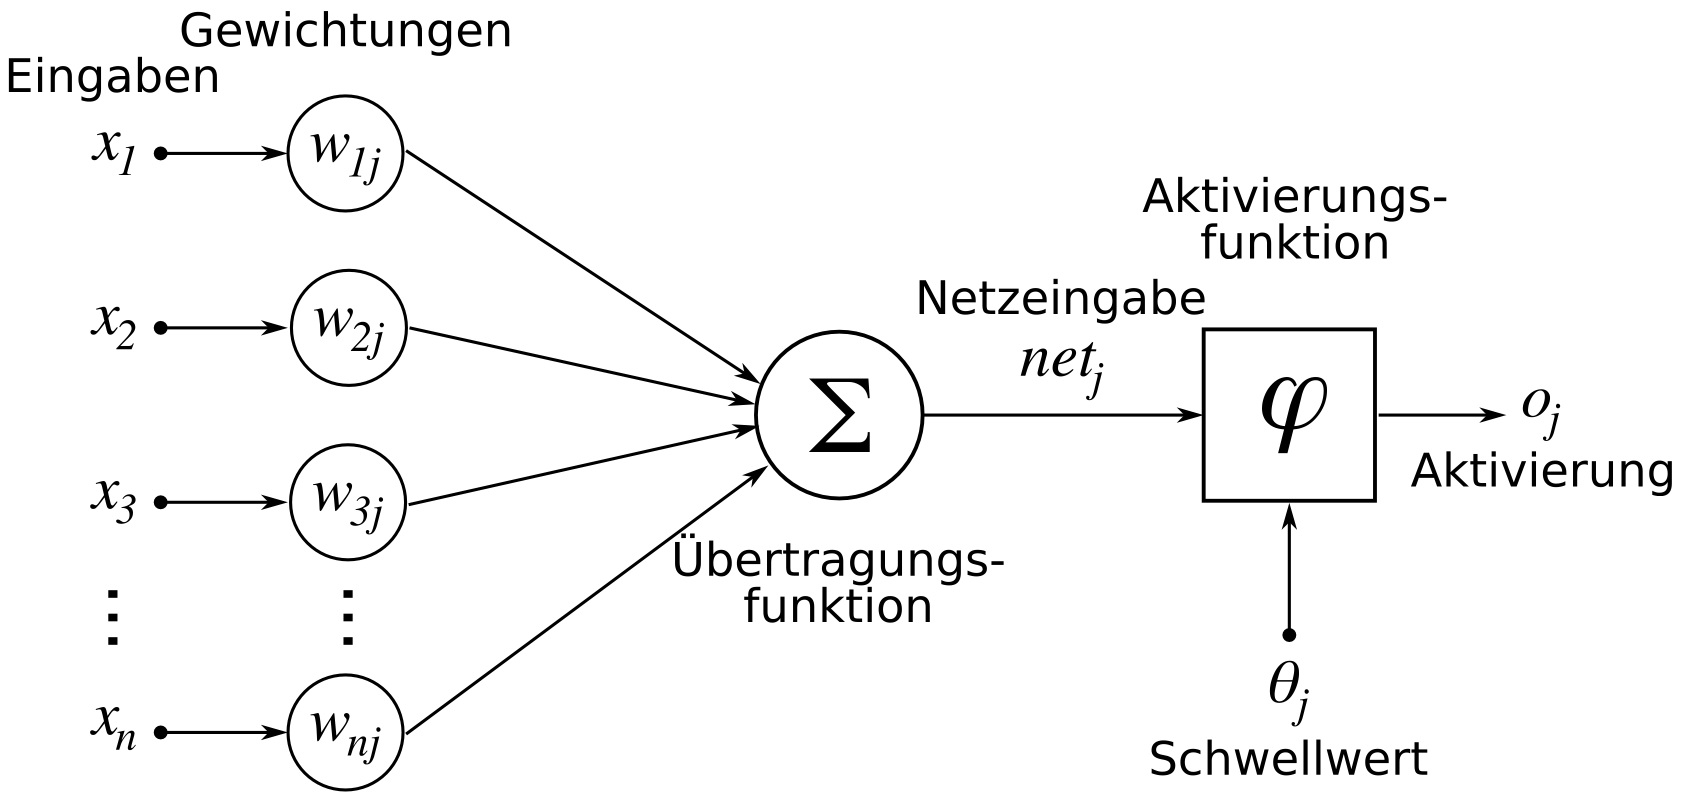
\includegraphics[width=8cm]{chapters/neural_networks/scheme.jpg}

\caption{Schematische Darstellung der wichtigsten Bestandteile eines künstlichen Neurons (Quelle: Wikipedia)}
	\label{img:scheme}

\end{figure}
Die Funktion der Dendriten erfüllen die Eingaben x$_i$, wobei i = 1, …, n. Beim Modellieren eines KNN sollte man nicht vergessen, dass die Länge eines Neurons eine große Rolle bei der Bestimmung der Signalstärke spielt. Dies wird durch die Gewichtungen w$_i$$_j$ dargestellt. Die Gewichtung wird mit dem Eingabewert multiplikativ verknüpft. Es gibt verschiedene Vorgehenstechniken bei der Belegung der Gewichtungen, aber häufig werden dafür zufällige Werte in einem bestimmten Wertebereich ausgesucht. Je nachdem, ob die Gewichtung einen positiven oder einen negativen Wert hat, wirkt der Transmitter entweder verstärkend oder hemmend genau so wie bei den Menschen. Falls die Gewichtung gleich 0 ist, hat ein Neuron auf ein anderes Neuron keinen Einfluss.

Die Übertragungsfunktion könnte man sich als Erregungspotenzial vorstellen. In dieser Funktion, genauso wie die Signale im Zellkern, werden die Eingaben entsprechend ihrer Gewichtungen aufsummiert und zu einem Wert umgerechnet, damit man danach eine reellwertige Funktion darauf anwenden kann.
Der Schwellenwert $\theta$$_j$ dient als Schwellenpotenzial. Das Addieren eines Schwellwerts zur Netzeingabe verschiebt die gewichteten Eingaben.
Die Aktivierungsfunktion $\phi$ berechnet aus dem aktuellen Aktivierungszustand und der Netzeingabe den neuen Aktivierungswert. Dieser Wert wird dann weitergeleitet. Die Aktivierungsfunktion kann wie die echten Neuronen dem Alles-oder-gar-nichts-Prinzip folgen. Dabei wird bei der Überschreitung des Schwellenpotenzials wie bei menschlichen Neuronen ein festes Aktionspotential generiert. So eine Aktivierungsfunktion heißt auch Sprungfunktion (siehe Abb. 3.2).
\begin{figure}[h]
\centering
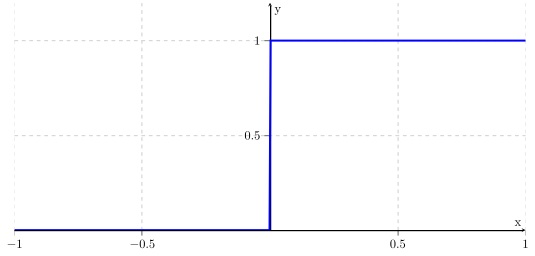
\includegraphics[width=5cm]{chapters/neural_networks/sprung.jpg}

\caption{Eine Sprungfunktion (Quelle: Wikipedia)}
	\label{img:sprung}

\end{figure}

 Eine Aktivierungsfunktion kann aber auch nach den anderen Prinzipien funktionieren. Häufig wird eine sogenannte Sigmoidfunktion (siehe Abb. 3.3) mit einer ungleichmäßigen Abhängigkeit zwischen der Ein- und Ausgabe verwendet. Weitere mögliche Aktivierungsfunktionen sind lineare oder stückweise lineare Funktionen (siehe Abb. 3.4). In solchen Funktionen hängt die Ausgabe linear von der Eingabe ab.


\begin{figure}[h]
\centering
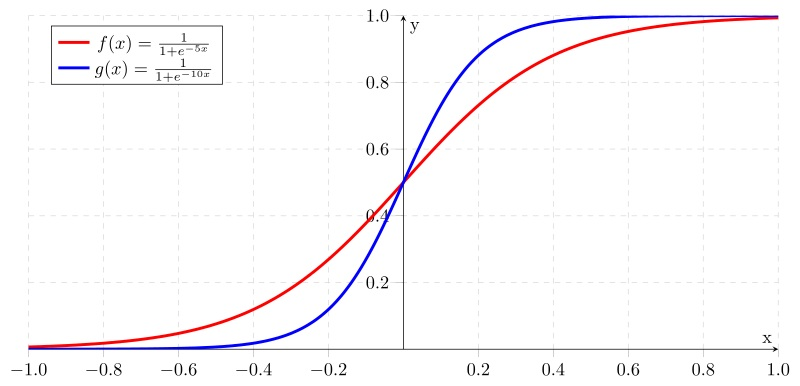
\includegraphics[width=5cm]{chapters/neural_networks/sigmoid.jpg}

\caption{eine Sigmoidfunktion mit  Steigerungsmaß (Quelle: Wikipedia)}
	\label{img:sigmoid}

\end{figure}

\begin{figure}[h]
\centering
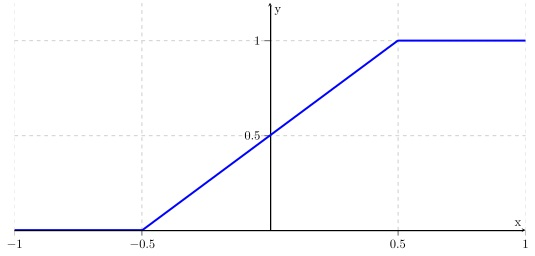
\includegraphics[width=5cm]{chapters/neural_networks/lin.jpg}

\caption{eine stückweise lineare Funktion (Quelle: Wikipedia)}
	\label{img:lin}

\end{figure}

Die Aktivierung o$_j$ ist das Ergebnis einer Aktivierungsfunktion und dient als „Ausgang“ eines künstlichen Neurons.

\subsection{Verbindungen und Netzwerktopologien}

Durch den Verbund von mehreren geordneten Kanten zwischen den Verarbeitungseinheiten entsteht ein KNN. Dabei wird die räumliche Anordnung dieser Einheiten als Netzwerktopologie bezeichnet.
Eine der wichtigsten Aufgaben der Verbindungen ist es die Architektur eines KNN festzulegen. In manchen Netzen entstehen durch solche Kanten sogenannte Schichten.

Die Verbindungen zwischen den Einheiten sind für die Kommunikation zwischen Neuronen verantwortlich: über diese Kanten werden die Daten ausgetauscht, wobei jede Verbindung durch einen Gewichtswert realisiert wird. Dabei unterscheidet man zwischen den unidirektionalen und bidirektionalen Verbindungen.

Durch unidirektionale Inter-Layer-Verbindungen werden die Daten der Eingabeschicht zur Ausgabeschicht weitergeleitet. Dadurch entstehen die sogenannten Feed-Forward-Netze, die man sich als einen azyklischen Graphen vorstellen kann.

Bidirektionale Verbindungen bilden die Feed-Backward-Netze. Bei den FB-Netzen unterscheidet man drei Typen:

a) later feedback: bidirektionale Verbindungen entstehen zwischen den Knoten einer Verarbeitungsschicht;

b) direct feedback/self-feedback: es entsteht eine unidirektionale Verbindung einer Einheit mit sich selbst;

c) indirect feedback: es entsteht eine bidirektionale Verbindung zwischen zwei Knoten aus zwei benachbarten Schichten.

Die Topologien lassen sich in drei Haupttypen unterscheiden:

a) Einschichtige Netze: solche Netze besitzen nur eine Ausgabeschicht und sind deswegen die einfachsten KNN Strukturen, die es gibt (siehe Abb. 3.5).

\begin{figure}[h]
\centering
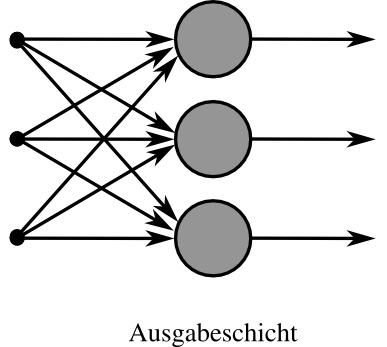
\includegraphics[width=3cm]{chapters/neural_networks/single.jpg}

\caption{Ein einschichtiges KNN (Quelle: Wikipedia)}
	\label{img:single}
\end{figure}


b) Mehrschichtige Netze: solche KNN verfügen neben der Ausgabeschicht auch über eine oder mehrere versteckte Schichten, die sich zwischen den Ein- und Ausgabeschichten befinden. Sie sind deshalb von außen nicht sichtbar (siehe Abb. 3.6).

\begin{figure}[h]
\centering
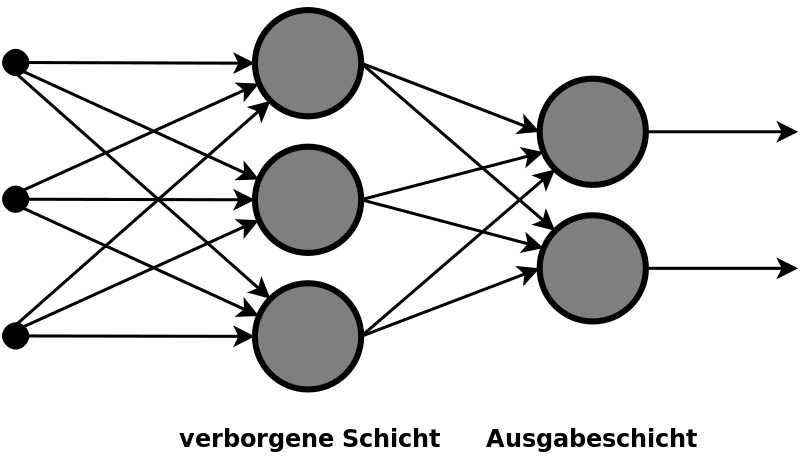
\includegraphics[width=4cm]{chapters/neural_networks/multilayer.jpg}

\caption{Ein mehrstufiges KNN mit einer verborgenen Zwischenschicht (Quelle: Wikipedia)}
	\label{img:multi}
\end{figure}

c) Rekurrente Netze: solche KNN verfügen über rückgekopellte Verbindungen, was zu Schleifen im Datenfluss führt (feedback loops). Dadurch wird der Ausgabewert eines Knotens als Eingabewert desselben Knotens verwendet (siehe Abb. 3.7).

\begin{figure}[h]
\centering
\includegraphics[width=3cm]{chapters/neural_networks/recurrent.jpg}

\caption{Ein rekurrentes KNN (Quelle: Wikipedia)}
	\label{img:recurrent}

\end{figure}

Aus diesen grundlegenden Netzwerktypen lassen sich gemischte Topologien bilden, wie z.B.: einschichtige/mehrschichtige vorwärtsbetriebene KNN (single-layer/multiple-layer feed-forward networks), Strukturen mit direkten und indirekten Rückkopplungen, Topologien mit lateralen Rückkopplungen (lateral feedback networks), usw.

\subsection{Lernregeln}

Lernregeln sind eines der wichtigsten Elemente in KNN. Ihre Aufgabe ist es dafür zu sorgen, dass das Netz aus Fehlern lernt. Beim Auftreten eines Fehlers werden die Gewichte und/oder die Topologie des KNN verändert.

\subsubsection{Hebbsche Lernregel}

Diese Regel wurde im 1949 von Donald Olding Hebb aufgestellt und gilt als universelles Lernprinzip eines KNN. Diese Regel besagt, dass, wenn zwei verbundene Neurone gleichzeitig aktiv sind, die Verbindung zwischen diesen Neuronen stärker ausgeprägt wird:

%\centering
$\Delta$w$_i$$_j$ = $\eta$a$_i$o$_j$ = $\eta$ $\cdot$ g(a$_i$, t$_i$) $\cdot$ h(o$_j$, w$_i$$_j$) ,
\newline
 wobei:  $\Delta$w$_i$$_j$ -- die Veränderung des Gewichtes zweier Neuronen i und j,  $\eta$ -- eine Lernrate (konstant), a$_i$ -- Aktivierung von Neuron i, o$_j$ -- Ausgabe von Neuron j.

Zusammen mit der Hebbschen Lernregel wird häufig eine binäre Aktivierungsfunktion benutzt. Dabei werden die Aktivierungen auf $1$ oder $-1$ festgelegt. Das resultiert entweder in einer positiven Verstärkung oder in einer Verringerung der Gewichte, falls beide Neuronen nicht übereinstimmen.
\subsubsection{Delta-Regel}

Die Delta-Regel gilt als Weiterentwicklung der Regel von Hebb und berücksichtigt die Differenz zwischen der erwarteten Aktivierung t$_i$ (teaching output) und der tatsächlichen Aktivierung a$_i$:

$\Delta$w$_i$$_j$ = $\eta$$\delta$$_i$o$_j$ = $\eta$(t$_i$ $-$ a$_i$)o$_j$ .

 Diese Regel wird nur zusammen mit den linearen Aktivierungsfunktionen eingesetzt.

\subsubsection{Backpropagation-Regel}

Dieses Verfahren dient zum Einlernen von KNN und ist die Verallgemeinerung der Delta-Regel für die mehrstufigen Strukturen.
KNN versuchen die Erkennungsfehler zu minimieren, indem sie jedes Mal die Abweichung von der Lösung durch das Netz rückwärts laufen lassen. Dadurch wird das KNN so angepasst, dass die Fehler besser erkannt werden.

Die standardisierte Delta-Regel führt bei zu kleinen Abweichungen zu keiner ausreichenden Informationstiefe und ist durch die Abhängigkeit von linearen Aktivierungsfunktionen in ihrer Anwendung beschränkt. Zur Lösung dieses Problems wird die Sigmoidfunktion, die selbst kleinste Abweichungen mit nichtlinearen Aktivierungsfunktionen warhnehmen kann, zur Anpassung der Delta-Regel zu Hilfe genommen.

$\Delta$w$_i$$_j$ = $\eta$$\delta$$_i$o$_j$,
\newline
wobei
\begin{figure}[h]
\centering
\includegraphics[width=6cm]{chapters/neural_networks/delta.jpg}

\end{figure}
\section{Beispiele}
\subsection{Das Perzeptron}
Im Jahr 1958 entwickelte Frank Rosenblatt das sogenannte Perzeptron: ein Modell, das praktisch fast alle logischen Funktionen berechnen kann. Man unterscheidet zwischen einlagigen und mehrlagigen Perzeptronen.

\subsubsection{Einlagiges Perzeptron}
\begin{figure}[h]
\centering
\includegraphics[width=3cm]{chapters/neural_networks/perzeptron.jpg}

\caption{Ein einlagiges Perzeptron}
\label{preceptron}

\end{figure}
Diese Art Perzeptronen besteht aus einer einzigen Schicht, die gleichzeitig den Ausgabevektor repräsentiert. Auf der Abbildung \ref{preceptron} ist ein einlagiges Perzeptron dargestellt. Als Eingabe bekommt es den Eingabevektor (x$_1$, ..., x$_n$).

Das Perzeptron besitzt auch einen Gewichtsvektor (w$_1$, ..., w$_n$) und einen Schwellwert $\theta$.

Aus dem Eingabe- und Gewichtsvektor berechnet man das Skalarprodukt, und wenn das Ergebnis größer oder gleich dem Schwellwert ist, dann „feuert“ unser Perzeptron.

Als Beispiel betrachten wir nun ein binäres einlagiges Perzeptron, welches eine AND-Funktion modellieren kann (siehe Abb. \ref{orfct}).
Bei einer binären Eingabe besteht unser Eingabe- bzw. Gewichtsvektor nur aus zwei Werten.
Die erwartete Ausgabe wird als eine Tabelle in der Abbildung \ref{orfct} dargestellt.
Unser Neuron soll nur dann „feuern“, wenn das Ergebnis 1 ist, deswegen ist es sinnvoller die beiden Gewichte auf 1 zu setzen.
Der Ausgabewert y$\in$$\{$0, 1$\}$, wobei y folgendermaßen definiert ist:
\begin{equation*}
y =
\begin{cases}
1, <x,w> \geq 0\\
0, \text{sonst}
\end{cases}
\end{equation*}

\begin{figure}[h]
\centering
\includegraphics[width=7cm]{chapters/neural_networks/and.jpg}

\caption{Das Perzeptron-Modell einer AND-Funktion}
\label{orfct}

\end{figure}
\begin{figure}[h]
\centering
\includegraphics[width=3cm]{chapters/neural_networks/linearsep.jpg}

\caption{Linear separierbare Ergebnisse einer AND-Funktion}
\label{linseporfct}

\end{figure}

Man sollte dabei erwähnen, dass einlagige Perzeptrone nur auf linear separierbaren Datensätzen gute Ergebnisse liefern. Linear separierbar bedeutet, dass man die Ergebnisse mit einer Linie in richtig oder falsch separieren kann. Die Abbildung \ref{linseporfct} repräsentiert vier mögliche Ergebnisse aus unserem OR-Beispiel und zeigt, wie sie voneinander durch eine Hyperebene separiert werden können.


\subsubsection{Mehrlagiges Perzeptron}

Mehrlagige Perzeptrone bestehen aus mindestens zwei Schichten (einer Ausgabeschicht und einer/mehreren versteckten Schicht/-en). Dabei sind alle Neuronen einer Schicht mit den Neuronen einer anderen Schicht verbunden. So eine Topologie ermöglicht die Probleme zu lösen, bei den einlagige Perzeptrone gescheitert sind.

\subsection{Perzeptron-Lernregel}

Die Lernregel eines binären einlagigen Perzeptrons könnte man folgendermaßen definieren:
\newline
w$_i$$_j$(neu) = w$_i$$_j$ (alt) $\pm$ $\Delta$w$_i$$_j$,
\newline wobei $\Delta$w$_i$$_j$ die Änderung des Gewichts w$_i$$_j$ ist. Das bedeutet:
\begin{itemize}
\item Wenn das Ergebnis 1 und der Ausgabewert 1 sein soll, dann werden die Gewichte nicht geändert (das gleiche gilt für 0).
\item Wenn das Ergebnis 0 und der Ausgabewert 1 sein soll, dann werden die Gewichtungen inkrementiert.
\item Wenn das Ergebnis 1 und der Ausgabewert 0 sein soll, dann werden die Gewichtungen dekrementiert.
\end{itemize}

Als Beispiel betrachten wir die Funktion aus der Abbildung \ref{perceptronlearning}.

\begin{figure}[h]
\centering
\includegraphics[width=10cm]{chapters/neural_networks/schritt1.jpg}

\caption{Eingabevektoren und Initialisierung des Gewichtsvektors}
\label{perceptronlearning}

\end{figure}

Als erstes initialisieren wir den Gewichtsvektor und den Schwellenwert mit Nullen und berechnen die erwarteten Ausgabewerte. Danach berechnen wir das Skalarprodukt von den Gewichtungen und dem 1. Eingabevektor (siehe Abb. \ref{perceptronlearningsteps}, Schritt 2). Die erwartete Ausgabe ist 1, wir bekommen aber 0 raus, deswegen müssen wir die Werte unseres Gewichtsvektors inkrementieren. Im Schritt 3 berechnen wir das Skalarprodukt von unserem neuen Gewichtsvektor und dem 2. Eingabevektor. Der Ausgabewert stimmt mit dem erwarteten Wert überein, deswegen müssen wir nichts ändern. Die gleiche Berechnung machen wir für den 3. Eingabevektor (Schritt 4) und merken, dass der Ausgabewert 0 statt 1 sein soll. Deswegen werden  die Werte des Gewichtsvektors dekrementiert. Das gleiche machen wir mit dem 4. Eingabevektor.

\begin{figure}[h]
\centering
\includegraphics[width=12cm]{chapters/neural_networks/schritte.jpg}

\caption{Schritte 2-5}
\label{perceptronlearningsteps}

\end{figure}

Wenn alle Eingabevektoren getestet wurden, fängt der neue Zyklus an. Im neuen Zyklus werden die gleichen Berechnungen durchgeführt, bis die passenden Gewichte gefunden sind.


\section{Fazit}

In dieser Ausarbeitung haben wir die Grundlagen und die wichtigsten Bausteine Künstlicher Neuronaler Netze kennengelernt. Zusammenfassend kann man sagen, dass KNN lernfähig sind und im Vergleich zu regelbasierten Expertensystemen keine Menschen  benötigen, die explizit beschriebene Regeln erstellen müssen. Sie sind in der Lage die Gewichtswerte und ihre Struktur an jedes Problem anzupassen und besitzen daher hohe Performanz und Adaptivitätsfähigkeit. Dank ihrer Anpassungsfähigkeit sind KNN in der Lage auch für nicht gelernte Eingaben korrekte Lösungen zu finden, deswegen hat dieses Verfahren eine Allgemeingültigkeit. KNN können nicht nur lineare, sondern auch nichtlineare Datensätze bearbeiten.

\section{Quellen und Literatur}
\begin{itemize}
\item David Kriesel. Ein kleiner Überblick über Neuronale Netze. (Online unter: \url{http://www.dkriesel.com})
\item \url{http://www2.cs.uni-paderborn.de/cs/ag-klbue/de/courses/ss03/kimas/project/downloads/AUSARBEITUNGEN/ThomasHeinenNNInMAS.pdf}
\item \url{https://de.wikipedia.org/wiki/Künstliches neuronales Netz}
\item \url{https://de.wikipedia.org/wiki/Perzeptron}
\item MIT - Lecture 12A: Neural Nets
\item MIT - Lecture 12B: Deep Neural Nets
\end{itemize}

\usetikzlibrary{calc}
\usetikzlibrary{positioning}
\usetikzlibrary{matrix}

\pgfdeclarelayer{background}
\pgfsetlayers{background,main}

\newtheorem{mydef}{Definition}
\newtheorem{algo}{Variante}

\chapterimage{chapter_head_1.png}
\chapter{Genetische Algorithmen}

\section{Intro \& Motivation}
Was bedeutet eigentlich Intelligenz?

Das ist eine Frage, auf die keiner eine absolut klare Antwort geben kann. Was wir aber mit Sicherheit wissen ist, dass wir Menschen uns als intelligent bezeichnen. Um nun also das Konzept der künstlichen Intelligenz besser zu verstehen und voran zu treiben, hat man sich -- ähnlich zu den neuronalen Netzen -- einen Ansatz überlegt, der sich an der Natur orientiert:
Genetische Algorithmen!

Dieser Typ Algorithmus verhält sich ähnlich zu den simplen Prinzipien der Genetik und wird häufig dafür genutzt, um Optimierungsprobleme zu lösen. Um euch dies näher zu bringen, werde ich im Folgenden das Prinzip, die Funktionsweise und Arbeitsbereiche von genetischen Algorithmen erläutern.

\section{Begriffe}
\begin{mydef}(Individuum)\\
	Ein Individuum ist einzelnes Element des großen Ganzen. Es ist nicht teilbar und ist das "`Ding"', was betrachtet wird. In der Biologie sind dies häufig die Zellen, aber hier werden Kandidaten für mögliche Lösungen eines Problems betrachtet.
\end{mydef}
\begin{mydef}(DNA)\\
	Die DNA ist die  Codierung sämtlicher Erbinformationen eines Individuums. Sie entspricht der Zusammenfassung aller Grundeigenschaften.
\end{mydef}
\begin{mydef}(Gen)\\
	Ein Gen ist ein Abschnitt der DNA. Es entspricht meist einer einzelnen Eigenschaft des Individuums, kann aber auch manchmal mehrere Eigenschaften umfassen.
\end{mydef}
\begin{mydef}(Population)\\
	Die Population ist die Menge aller betrachteten Individuen zu einem bestimmten Zeitpunkt.
\end{mydef}
\begin{mydef}(Genotyp/Phänotyp)\\
	Der Genotyp ist die Beschreibung eines Individuums in codierter Form. Der Phänotyp dagegen beschreibt das Individuum so, wie es ist, also durch seine Eigenschaften.
\end{mydef}
\begin{mydef}(Fitness)\\
	Die Fitness eines Individuums gibt dessen Güte/Stärke an. Von ihr hängen hauptsächlich die Überlebenschancen ab.
\end{mydef}

\section{Biologischer Hintergrund}
Im Folgenden werde ich kurz die Abläufe der Evolution auf biologischer Ebene erläutern. Dafür betrachte ich de Zellebene in Kombination mit der Vererbung, wie sie beim Menschen auftritt.

Jede Zelle hat eine eigene DNA (Desoxyribonucleinsäuren) im Kern, die sämtliche Informationen speichert. Diese ist aus verschiedenen Basenpaaren zusammengesetzt, die wie Puzzelteile ineinander passen. Die Gene sind Teilabschnitte der DNA und sind eine Codierung für je eine Eigenschaft. Bespiele sind helle Haut oder blaue Augen. Die Allele sind jeweils Paare von 2 Genen, die zu ein und derselben Eigenschaft gehören. Dabei stammt je ein Gen vom Vater und eines von der Mutter.

Es gibt verschiedene Arten von Erbgängen. Ich werde im Folgenden zunächst den dominant-rezessiven Erbgang erklären:
Dabei ist ein Gen dominant und das andere rezessiv, was bedeutet, dass sich das dominante durchsetzt und letztendlich für die bestimmte Eigenschaft verantwortlich ist. Es sind aber beide Gene in der DNA enthalten. Bei der Reproduktion wird sowohl beim Vater, als auch der Mutter von jedem Allel eines der Gene ausgewählt und dann zu einem neuen Allel kombiniert. Dies kann dazu führen, dass beispielsweise zwei rezessive Gene zusammenkommen und sich dann im Kind eine Eigenschaft durchsetzt, die keines der beiden Elternteile besaß.

Nun folgt der intermediäre Erbgang:
Hierbei haben die Gene verschiedene Werte und bei der Vererbung überlagern sich diese. Hat man zum Beispiel zwei Blumen, von denen eine weiß und die andere rot ist, so kann die Kreuzung der beiden eine rosa Blume hervorbringen.

Es können zufällige Veränderungen in der DNA einer Zelle auftreten. Dies kann zum Beispiel durch äußere Einflüsse, wie radioaktive oder ultraviolette Strahlung auftreten. Die Zellen versuchen meist diese Veränderung rückgängig zu machen, gelingt dies jedoch nicht, so ist eine Mutation in der Zelle aufgetreten. Dies kann unter anderem auch zu Krankheiten wie Krebs führen. Die Mutationen werden auch bei der Vererbung weitergegeben.

Die Selektion basiert auf dem Überleben des Stärkeren. Dies kann sich in vielen verschiedenen Dingen äußern. Einige Beispiele sind Anpassungsfähigkeit bei Veränderung der Umweltbedingungen, Stärke beim Kampf um Nahrung, Schnelligkeit und Wendigkeit, strategisches Handeln. Dabei kann es auch Vor- oder Nachteile durch gewisse Mutationen geben.

Ein weiterer Faktor ist hierbei auch die Nahrungskette. Die Lebewesen, die höher in der Nahrungskette stehen, setzen sich oft gegenüber den Schwächeren durch, da sie diese einfach fressen. Dies bedeutet aber nicht unbedingt, dass sie überleben, wenn sie nicht so anpassungsfähig sind, wie andere.

Beim Menschen tritt die natürliche Selektion jedoch kaum noch auf. Dies kommt daher, dass wir Menschen versuchen alle Leute aufzufangen, indem wir ein soziales Konstrukt aufgebaut haben. Dabei ist es das Ziel, dass jeder mit den lebensnotwendigen Dingen versorgt wird und eine Chance hat sich in die Gesellschaft einzubringen.

\section{Ablauf}
Das Ziel eines genetischen Algorithmus ist die Optimierung der Fitness aller Individuen in einer Population. Dies wird durch langfristige Weiterentwicklung in einem Zyklus erreicht.
Es startet mit einer Anfangspopulation, die sich durch Vererbung immer weiter entwickelt. Man fängt damit zunächst mit einer Betrachtung des Genotyps an.

Der erste Schritt ist die Mutation einzelner Stellen in den Genen der Individuen.
Darauf folgt dann eine Kreuzung der Individuen zu jeweils neuen Nachkommen. Dafür werden die Gene zweier Individuen zunächst aufgespalten und dann neu kombiniert. Dies kann auf verschiedene Arten geschehen. Man kann z.~B. den Anfang des ersten mit dem Ende des zweiten Gens kombinieren.
Dann wird der Phänotyp betrachtet. Dieser wird mit Hilfe einer Fitness-Funktion bewertet und anhand dieser, werden die Überlebenschancen für ein Individuum festgelegt.
Zuletzt findet dann die Selektion statt. Dabei werden aus sämtlichen neu entstandenen Individuen die "`besten"' ausgewählt, um die nächste Generation zu bilden. Mit dieser kann dann wieder von vorne begonnen werden.

Dies wird solange wiederholt, bis man sein Ziel erreicht hat oder es keinen Fortschritt mehr zu beobachten gibt. Dies kann aufgrund verschiedener Probleme, die später noch genauer erläutert werden, auftreten.

\section{Codierung}
Um die Individuen gut betrachten und später reproduzieren zu können muss man eine anschauliche Darstellung für die Gene wählen. Diese Wahl hängt hauptsächlich vom gegebenen Problem ab und kann deshalb nicht allgemein angegeben werden. Dennoch werde ich einige grundlegende Prinzipien zur Codierung darstellen.

\subsection{Binärcodierung}
Die Binärcodierung ist eines der ältesten Konzepte und beruht auf der Darstellung von Zahlen im Binärsystem. Dabei haben die Gene immer eine feste Länge und die Stellen darin sind entweder 0 oder 1. Die Bedeutung der Gene lässt sich im Genotyp zunächst nicht erkennen (dies ist im Allgemeinen unabhängig von der Codierung), kann aber nach der Umwandlung in den Phänotyp erkannt werden. So kann zum Beispiel eine 1 an einer Stelle dafür stehen, dass das Individuum eine bestimmte Eigenschaft besitzt, und eine 0, dass diese nicht vorhanden ist. Ein anderes Beispiel ist, dass die Gene einfach als Binärzahlen interpretiert werden und sich somit eine Zahl als Phänotyp ergibt.

Die Binärcodierung in Kombination mit der Interpretation als Zahlen kann aber auch zu Problemen führen. Mutiert man zum Beispiel bei einer 10-stelligen Binärzahl die erste Stelle erreicht man eine Änderung von 512 im Ergebnis, bei einer Mutation in der letzten Stelle jedoch nur um 1. Daher haben die Mutationen eine stark schwankende Bedeutung im Ergebnis zu Folge. Um dies auszugleichen bräuchte man einen großen algorithmischen Aufwand.

Ein weiterer Kritikpunkt ist, dass bei Kreuzungen das Elternteil, das für den vorderen Teil zuständig ist, einen deutlich höheren Einfluss auf die nächste Generation hat, als der hintere Teil. Dies sollte aber möglichst vermieden werden.

Ein Lösungsansatz für diese beiden Probleme ist die Verwendung des Gray Codes. Dieser hat im Gegensatz zum Binärcode den Vorteil, dass benachbarte Codewörter eine Hamming-Distanz von 1 haben, sich also zwei benachbarte Zahlen im Phänotyp, im Genotyp an nur einer einzigen Stelle unterscheiden.

\subsection{Realzahl Codierung}
Bei dieser Art der Codierung werden die Gene als reelle Zahlen aufgefasst. Im Gegensatz zur Binärdarstellung ist die Länge der Gene hier -- zumindest theoretisch -- nicht fest. In der Umsetzung ist es oft aber leichter eine feste Länge zu verwenden, was dann zu einer Darstellung as Fließkommazahlen führt.

Diese Darstellung wird oft verwendet, wenn kontinuierliche statt diskrete Probleme betrachtet werden.


\section{Reproduktion}
Im Zuge der Reproduktion werden einerseits die Gene der einzelnen Individuen mutiert und andererseits zwei Individuen zu einem neuen gekreuzt. Dabei gibt es mehrere Faktoren zu beachten, die im Folgenden erläutert werden:
\subsection{Kreuzung}
Da es oft mehrere Eigenschaften gibt, die zur Güte eines Individuums beitragen, aber nicht unbedingt ein einzelnes Individuum perfekt in allen Eigenschaften ist, ergibt es Sinn mehrere gute Individuen zu kombinieren. Da aber im Allgemeinen nicht klar erkennbar ist, welcher Teil des Gens für die Fitness positiv oder negativ verantwortlich ist, gibt es auch hier keine perfekte allgemeine Lösung als Schema zur Kreuzung. Ich werde aber dennoch mehrere Verfahren vorstellen:
\setcounter{algo}{0}
\begin{algo}(1-Punkt-Crossover)\\
	Bei diesem Verfahren werden die Gene der beiden Eltern an jeweils einer Stelle geteilt. Die Gene der Nachfahren ergeben sich dann dadurch, dass der erste Teil des einen Elternteils mit dem zweiten Teil des anderen kombiniert wird und umgekehrt. Wenn zum Beispiel das erste Individuum einen sehr guten ersten Teil des Gens besitzt, aber der zweite Teil des zweiten ist überragend, so kann die Kombination der beiden ein hervorragendes Ergebnis sein und die beiden Vorgänger um vieles überragen.
\end{algo}

\begin{algo}(N-Punkt-Crossover)\\
	Dies kann man als Verallgemeinerung des 1-Punkt-Crossovers verstehen. Dabei werden die Gene in mehr als 2 Teile aufgespalten und die Nachkommen erhalten dann alternierend die Teile der Eltern.
\end{algo}

\begin{algo}(Uniform Crossover)\\
	Dieses Verfahren unterscheidet sich von den beiden anderen dadurch, dass die Eltern nicht in Teile aufgespalten werden. Hierfür wird zu jeder einzelnen Stelle eine Wahrscheinlichkeit berechnet, ob sie ausgetauscht wird. Ist diese größer als 0,5 werden die Stellen getauscht und sonst nicht. Dadurch ergeben sich die Nachkommen.
\end{algo}

\begin{algo}(Mittelung)
	Dieser Algorithmus lässt sich gut bei reellwertiger oder ganzzahliger Codierung anwenden. Um von den Eltern auf einen Nachkommen zu kommen wählt man hier -- ähnlich zum intermediären Erbgang -- jeweils das Mittel der beiden Stellen in den Genen um den Wert an der entsprechen Stelle im Gen des Nachkommens zu berechnen.
\end{algo}

\subsection{Mutation}
Die Mutationen sind wichtig um eine höhere Varianz in die Population einzubringen. Hat zum Beispiel die Startpopulation nur Individuen mit demselben Genotyp und die Länge der Gene ist fest, so kann ohne Mutationen keine Veränderung im Genotyp, also auch im Phänotyp stattfinden, weshalb man zu keiner Lösung des Problems kommt.

Eine Möglichkeit zur Mutation ist die Veränderung einzelner Stellen in den Genen.  Anhand einer vorher festgelegten Mutationsrate wird bestimmt, ob die betrachtete Stelle gleich bleibt, oder verändert werden soll. Tritt eine Veränderung auf, so wählt man ein anderes Codewort aus, welches nun dieser Stelle zugewiesen wird. Man kann auch die maximale/minimale Anzahl der Mutationen in einem Gen oder sogar der gesamten Population festlegen, um die Mutationen gezielt zu steuern.

Die Wahl des neuen Codeworts kann auf mehrere Arten realisiert werden. Eine Möglichkeit ist eine komplett zufällige Wahl des neuen Codeworts und eine andere eine Änderung um einen kleinen Wert.

Man sollte jedoch vorsichtig bei der Wahl der Mutationsrate sein, da sonst auch Probleme auftreten können. Wählt man die Mutationsrate zum Beispiel zu hoch, kann es sein, dass die Kreuzung der besten Individuen gar keinen Effekt mehr hat, weil sie vorher bereits zu sehr verändert wurden und sich somit deutlich verschlechtert haben.

Eine andere Variante zur Mutation der Gene ist die Mutation durch Permutation. Dabei gibt es mehrere Varianten und hier werden 3 davon kurz vorgestellt:
\setcounter{algo}{0}
\begin{algo}(Swap Mutation)\\
	Hierbei werden zunächst zufällig 2 Positionen im Genotyp bestimmt und dann die Werte an den Stellen getauscht.
\end{algo}
\begin{algo}(Insert Mutation)\\
	Man bestimmt wieder 2 zufällige Positionen. Dann wird der Wert an der 2. Position direkt hinter den an der 1. verschoben und die restlichen werden jeweils um eine Position nach hinten verschoben, bis man an der 2. Position angelangt ist. Eine Voraussetzung dafür ist, dass die erste Position vor der zweiten liegt.
\end{algo}
\begin{algo}(Scramble Mutation)\\
	Der Algorithmus wählt hier wieder zwei Stellen im Gen aus und vertauscht dann zufällig alle Positionen zwischen diesen beiden. Die anderen Stellen im Gen bleiben dabei unverändert.
\end{algo}

\section{Fitness-Funktion}
Die Fitness-Funktion ist einer der wesentlichsten Bestandteile eines genetischen Algorithmus. Sie bewertet die Brauchbarkeit eines Individuums bezüglich des zu lösenden Problems und ist notwendig um später die Überlebens-/Fortpflanzungschancen festzulegen. Eine der gängigsten Varianten ist, die proportionale Fitness $\frac{B_x}{B_{gesamt}}$, die die Brauchbarkeit $B_x$ eines Individuums x in direkte Proportion zur Brauchbarkeit aller Individuen setzt. Da die genaue Form dieser Funktion stark vom zu lösenden Problem abhängt, kann man jedoch keine allgemeine Form angeben. Daher ist die Definition einer geeigneten Fitness-Funktion auch eines der größten Probleme beim Entwurf eines genetischen Algorithmus. Man kann jedoch im Allgemeinen sagen, dass es sinnvoll ist, keine Werte kleiner als 0 zuzulassen, da es sonst, wie wir später sehen werden, leicht zu Problemen kommen kann.

Man kann die Fitnessfunktion auch anpassen, um die Bedingungen zur Laufzeit des Algorithmus anzupassen:

So kann man die Fitnessfunktion $f$ zum Beispiel zeitabhängig machen, indem man $f^*=f^{k(t)}$ als neue Fitnessfunktion wählt. Der zeitabhängige Exponent k(t) steuert dann den Selektionsdruck, bewirkt also eine Anpassung der Verteilung der Überlebenswahrscheinlichkeit.

Eine weitere Variante dafür ist die sogenannte Boltzmann-Selektion. Dabei wählt man als neue Fitnessfunktion $f^*=exp(\frac{f}{kT})$. Dabei ist $T$ ein zeitabhängiger Temperaturparameter. Er fängt bei einem relativ hohen Wert an und fällt dann immer weiter ab. Dies hat zur Folge, dass mit steigender Zeit immer größere Unterschiede in der Fitnessfunktion auftreten, wodurch der Selektionsdruck immer weiter gesteigert wird. $k$ ist dabei eine Normierungskonstante.

\section{Selektion}
Wir haben nun bereits die Individuen nach ihrer Fitness bewertet, aber nun stellt sich die Frage:
Wie wirkt sich das eigentlich aus?

Es gibt verschiedene Ansätze von der Fitness zur Überlebenswahrscheinlichkeit zu kommen und ich möchte euch drei davon vorstellen:

Im Folgenden bezeichne ich mit $f(x)$ die Fitness eines Individuums $x$ und mit $P(x)$ dessen Überlebenswahrscheinlichkeit. Dabei ist die aktuelle Population die Menge $\{x_1,x_2,\dots,x_n\}$. (Achtung! Es ist auch möglich, dass nicht nur die Kinder, sondern auch die Eltern in die nächste Generation übernommen werden. Dies nennt sich "`steady state"'.)
\setcounter{algo}{0}
\begin{algo}\ \\
	Eine Möglichkeit ist ein simpler Stochastischer Ansatz:
	
	$$P(x_j)=\frac{f(x_j)}{\sum_{i=1}^{n}f(x_i)}$$
	
	Dabei wird die Fitness eines einzelnen Individuums ins Verhältnis zu der Summe der Fitness aller Individuen der aktuellen Population gesetzt. Dabei ergibt sich mit geeigneter Fitnessfunktion ein Wert zwischen 0 und 1, also eine gültige Wahrscheinlichkeit und somit eine Überlebenswahrscheinlichkeit.
	
	Hierbei können jedoch mehrere Probleme auftreten:
	
	\begin{enumerate}
		\item Wenn die Fitnessfunktion negative Werte zulässt, dann könnte $P(x_j)$ undefiniert sein, weil $\sum_{i=1}^{n}f(x_i)=0$ nicht ausgeschlossen ist.
		\item Für $P(x_j)$ sind negative Werte nicht ausgeschlossen, was dann keine gültige Wahrscheinlichkeit mehr ergibt.
		\item Bei einer sehr großen Population fallen einzelne Individuen mit relativ gesehen sehr großer Fitness gegebenenfalls gar nicht auf und deren Überlebenswahrscheinlichkeit ist trotzdem sehr gering.
	\end{enumerate}
\end{algo}
Um diese Probleme zu lösen kann man nun einen etwas anderen Ansatz wählen:
\begin{algo}(Ranked-Fitness-Selection)\\
	Das Individuum mit der größten Fitness sollte die besten Überlebenschancen haben, damit ein optimaler Wert erreicht werden kann. Dafür ordnet man die Individuen zunächst in absteigender Reihenfolge nach ihrer Fitness. Dann legt man einen Startwert $P_s$ als maximale Überlebenswahrscheinlichkeit fest. Die Überlebenswahrscheinlichkeit für $x_i$ berechnet sich dann als:
	
	\begin{center}
	$P(x_i)=\begin{cases}
	P_s & \mathrm{falls~} i=1\\
	(1-P_s)P(x_{i-1}) & \mathrm{sonst}
	\end{cases}$
	\end{center}
	
	Damit erhält man in jedem Fall eine gültige Wahrscheinlichkeit und die besten Individuen haben eine deutlich höhere Überlebenswahrscheinlichkeit als der Rest.
	
	Ein Problem bleibt aber bestehen:
	Lokale Maxima in der Fitnessfunktion können schnell dazu führen, dass kein Fortschritt mehr auftritt und der Algorithmus somit nicht mehr funktioniert.
\end{algo}
Um dieses Problem zu umgehen muss eine hohe Varianz in der neuen Population gesichert werden. Dafür kann man folgenden Ansatz verwenden:
\begin{algo}(Uniform-Fitness-Selection)\\
	Man bewertet im Folgenden nicht mehr ausschließlich nach der höchsten Fitness eines Individuums, sondern zieht dabei auch die Vielfalt der nächsten Generation in Betracht. Das optimale Ergebnis wäre also eine Population mit sehr hoher Varianz und maximaler Fitness aller Individuen. Dafür bewertet man die Individuen nach folgendem Schema:
	\begin{figure}[h]
		\includegraphics[width=0.7\linewidth]{chapters/genetic/grafik.jpg}
	\end{figure}
	
	Der Startpunkt der Linien ist hierbei oben Rechts in der Ecke, also bei einem Maximum an Varianz und Fitness, also dem besten Individuum. Dabei symbolisieren die Linien einen immer weiteren Abstand zum Optimum und damit eine schlechtere Überlebenschance. Man sieht hier auch eine gewisse Abwägung zwischen Varianz und Fitness, da zum Beispiel bei der 5. Linie ein Individuum mit einer Fitness von nahezu 0 gleich bewertet wird wie eines mit maximaler Fitness, aber einer Varianz von nahezu 0.
	
	Ein Problem, das hierbei bestehen bleibt, ist, dass durch die hohe Varianz der Algorithmus nicht wirklich konvergiert. Dies kann man lösen indem man zunächst Uniform-Fitness-Selection betreibt und danach zur Ranked-Fitness-Selection wechselt
\end{algo}

\section{Anwendungsbereiche}
Ein theoretisches Anwendungsbeispiel ist das sogenannte Traveling-Salesman-Problem. Es geht dabei darum, dass ein Kaufmann von seinem Warenlager aus mehrere Stationen in einer Stadt beliefern und am Ende wieder zum Lager zurückkehren möchte. Dabei soll jede Station genau einmal besucht werden. Nummeriert man die Stationen mit 1 bis n durch, so erhält man eine Codierung für die Gene als Permutationen von 1 bis n. Die Fitnessfunktion ergibt sich dann als Kehrwert der Gesamtlänge des Weges. Bei der Reproduktion muss man jedoch vorsichtig sein, damit jedes mal gültige Permutationen entstehen. Dabei bietet es sich an eine Swap-Mutation durchzuführen. Die Kreuzung zweier Individuen erweist sich als komplizierter. Hier bietet es sich an ein Crossover durchzuführen, dann auf Gültigkeit zu testen und falls diese nicht vorhanden ist, das ganze rückgängig zu machen. Die entsprechenden Wahrscheinlichkeiten erhält man durch systematisches Probieren. Für die Selektion bietet sich dann die Ranked-Fitness-Selection an.

Genetische Algorithmen werden beispielsweise angewendet bei:
\begin{itemize}
	\item Konstruktion von komplexen Bauteilen
	\item Erstellung von Phantombildern
	\item Flugzeugbau
	\item Logistik (Ablaufplanung)
	\item Routenplanung
	\item Anordnungsprobleme
	\item Packprobleme
	\item Strategieprobleme (Spieltheorie)
	\item Parameteroptimierung
	\item Allgemein Optimierungsprobleme
\end{itemize}

Ein Beispielprogramm für die Logistik findet sich auf \href{http://www.dna-evolutions.com}{www.dna-evolutions.com}.

\section{Abgrenzung / Vergleich zu Neuronalen Netzen}
Ein Neuronales Netz ist ein Ansatz zur Lösung eines spezifischen Problems. Der Nachteil ist, dass man die Gewichte der einzelnen Knoten manuell durch Training anpassen muss. Genetische Algorithmen dagegen sind ein viel allgemeineres Prinzip, dass selbst optimale Lösungsansätze findet. So kann zum Beispiel auch ein genetischer Algorithmus verwendet werden, um ein neuronales Netz zu optimieren, oder sogar selbst zu entwerfen, indem er die Anzahl an Koten, Verbindungen und die Gewichte optimiert.\\

\section{Fazit \& Bewertung}
Genetische Algorithmen sind eine gute Möglichkeit um Optimierungsprobleme und Suchen mit großem Lösungsraum zu berechnen. Dabei werden im Gegensatz zu Expertensystemen keine weiteren Datenbanken oder ähnliches benötigt, sondern der Algorithmus verbessert sich immer weiter selbst. Der Nachteil ist, dass man in jedem  einzelnen Schritt stark vom Problem abhängige Wahlen treffen muss, die sich nicht unbedingt verallgemeinern lassen. Diese wirken sich dann stark auf den Ablauf des Programms aus und bestimmen das Ergebnis. Außerdem muss das Programm gegebenenfalls zur Laufzeit angepasst werden, entscheidet man  sich zum Beispiel das Selektionsverfahren zu ändern, damit eine Konvergenz des Algorithmus auftritt oder eine frühzeitige Konvergenz bei lokalen Maxima verhindert wird. Dennoch sind genetische Algorithmen eine sehr gute Alternative zum "`Brute Force"' Ansatz, da zum Finden einer Lösung nur ein kleiner Bruchteil des gesamten Lösungsraums betrachtet werden muss und das Programm mit einer gewissen Intelligenz nach einer Lösung sucht, anstatt blind alles auszuprobieren. Ein Problem bleibt jedoch, welches ist, dass immer nur eine Approximation und keine exakte Lösung berechnet wird. Daher muss man vorher abwiegen, ob dies ein guter Ansatz ist.

\section{Quellen und Literatur}

\href{http://www2.cs.uni-paderborn.de/cs/ag-klbue/de/courses/ws04/ea/students/ga_report.pdf}{(Skript Uni Paderporn)}\\
\href{http://www.mathematik.tu-dortmund.de/papers/MehmetiAmreinKulmsMacinLoenserBogonosWaidhas2014.pdf}{(Skript TU Dortmund)}\\
\href{http://www.spinfo.phil-fak.uni-koeln.de/fileadmin/spinfo/ki10/Genetische_algorithmen.pdf}{(Skript Uni Köln)}\\
\href{http://www.borgelt.net/slides/ga.pdf}{(Otto-von-Guericke-Universität )}
\href{http://www-e.uni-magdeburg.de/harbich/genetische_algorithmen/genetische_algorithmen.pdf}{(Skript Uni Magdeburg)}
\href{https://www.youtube.com/watch?v=kHyNqSnzP8Y}{(Vorlesung des MIT)}\\
\href{https://www.youtube.com/watch?v=6l6b78Y4V7Y}{(Vortrag von Kickstarter)}\\
\href{http://www.spektrum.de/lexikon/neurowissenschaft/zelle/14161}{(Spektrum Artikel zu Zellen)}\\
\href{http://www.spektrum.de/lexikon/biologie/genom/27365}{(Spektrum Artikel zu Genom)}\\
\href{http://semantic-web-grundlagen.de/w/images/e/e9/IntroAI-V06.pdf}{(Semantic Web)}\\
Grafik von Denis Krzysztala\\


\part{Sensorik \& Interaktion}
\chapterimage{chapter_head_1.png}

\chapter{Objekterkennung und Computer Vision}
\section{Intro \& Motivation}
Wie können wir uns eigentlich in der Welt, in der wir sind, zurechtfinden? Die \textbf{Wahrnehmung} ermöglicht die Aufnahme von Informationen über die Umgebung. Der Menschen hat fünf Hauptwahrnehmungssinne: Sehen, Hören, Tasten, Riechen und Schmecken. Können wir einer künstlichen Intelligenz (KI) diese Wahrnehmung beibringen? Wenn ja, wie?

Sinne bei KIs nennen wir \textbf{Sensoren}. Solche, die wir in KIs einbauen können, sind Sehen, Hören und Tasten. \textbf{Sehen} ist dabei im Hinblick auf den Gebrauch von KIs in der physischen Welt für uns Menschen der hilfreichste von allen.

In dieser Ausarbeitung werden zunächste Grundlagen über die Funktionsweise des Sehens beschrieben. Der Fokus wird dann auf die Verarbeitung von gewonnenen Rohinformationen liegen und ein paar Anwendungen ansprechen.

\section{Überblick Computer Vision}
Die Frage die Computer Vision stellt, ist eigentlich recht einfach: Wenn ein von der Umgebung ausgelöster Sensor-Impuls (S) so und so aussieht, wie sieht dann die Umgebung (W) dazu aus? Leider ist das Invertieren dieser Funktion
\begin{equation*}
S = f(W) \Rightarrow W = f^{-1}(S)
\end{equation*}
nicht so einfach möglich. Man muss sich also überlegen, anhand welcher Merkmale Entscheidungen über den Inhalt eines Bildes getroffen werden können. Computer Vision lässt sich dafür grob in drei Stufen einteilen:
\begin{itemize}
\item \textit{Low-Level Vision}: Grundlegende Untersuchung des Bildes auf herausstechende Features wie Unterschiede in Helligkeit, Farben oder Texturen und die damit verbundene Kantendetektion
\item \textit{Medium-Level Vision}: Objekterkennung und Bewegungsanalyse mithilfe der zuvor gesammelten Informationen
\item \textit{High-Level Vision}: Die Kombination und Analyse aller Daten: Was sagt mir das Bild, wie reagiere ich darauf?
\end{itemize}

Die Hauptanwendungsgebiete hierfür sind:
\begin{itemize}
\item Manipulation: Die Erlangung von benötigen Informationen von und Rückmeldung über lokale Gebilde, um mit diesen zu interagieren (z.~B.\ greifen, einfügen; Anwendung: z.~B.\ Qualitätskontrolle).
\item Navigation: Die Berechnung der eigenen Geschwindigkeit und Position (Ausrichtung), um Routen zu planen und Hindernissen auszuweichen.
\item Objekterkennung: Die Charakterisierung von Objekten zur Unterscheidung von \glqq gut\grqq\ und \glqq schlecht\grqq\ (z.~B.\ Beute- und Raubtier, (un)genie"sbare Früchte, Bekannte und Fremde).
\end{itemize}

Wir werden uns hier nur mit Low-Level- und Medium-Level Vision beschäftigen.
Zunächst werden wir auf die Entstehung von Bildern, Bildverarbeitungsoperationen, nutzbare Hinweise in Bildern, optisch gesteuerte Manipulation und Navigation und schließlich verschiedene Ansätze zur Objekterkennung eingehen.

\subsection{Grundlagen der Bildentstehung}

Um Informationen über einen \textbf{Ort} zu erhalten, benötigen wir ein Bild. Um ein \textbf{Bild} (2D) zu erstellen, müssen wir \textbf{Sehen} (3D) können. Das Sehen, so wie es in unseren Augen passiert, ist sehr komplex. Vereinfacht können wir es jedoch  anhand einer Lochkamera erkl"aren - der Prozess ist ungef"ahr der Gleiche.

\subsubsection{Lochkamera}

\marginpar[Links]{\small{(wer mit diesem Prinzip bereits vertraut ist, kann die nächste Seite überspringen)}}

\begin{figure}[h]
\centering
\includegraphics[width=8cm]{chapters/computervision/Grafik_1_Lochkamera.JPG}
\caption{Geometrie der Bildentstehung in einer Lochkamera.}
\label{fig:1}
\end{figure}
Eine Lochkamera ist eine schwarze Box, die an ihrer Front nur durch einen Punkt Licht eindringen lässt, welcher auf die Bildebene (Wand parallel zur Front) trifft. Je nachdem, wie gro"s die Lochblende ist, gelangen weniger oder mehr Lichtstrahlen hindurch. Je kleiner das Loch ist, desto schärfer ist das Bild, vor allem bei Objekten, die einen kleinen Abstand zur Lochkamera haben. Sobald das Loch vergrö"sert wird, gelangen mehr Lichtstrahlen hindurch, also wird ein Punkt vom Objekt durch mehrere Lichtstrahlen auf die Bildebene geschickt und das Bild erscheint uns unscharf.
\begin{figure} [h]
\centering
\includegraphics[width=12cm]{chapters/computervision/Grafik_3_Lochkamera.JPG}
\caption{Größe der Lochblende beeinflusst die Schärfe (links), der Abstand vor der Lochblende beeinflusst die Projektionsgrö"se (rechts).}
\label{fig:3}
\end{figure}

Wir betrachten einen Punkt $p$ mit den Koordination $(x,y,z)$ und seine \glqq Kopie\grqq\ $p'=(x',y',z')$ auf der Bildebene. $f$ beschreibt den Abstand zwischen der Lochblende $l$ und der Bildebene $b$.
\begin{figure}[h]
\centering
\includegraphics[width=8cm]{chapters/computervision/Grafik_2_Lochkamera.JPG}
\caption{Invertierte, gleiche Dreiecke.}
\label{fig:2}
\end{figure}
Es entstehen zwei kongruente Dreiecke, sodass wir die folgenden Umformungen vornehmen können:
\[\frac{-x'}{f}=\frac{x}{z},\quad \frac{-y'}{f}=\frac{y}{z} \quad \Rightarrow \quad x'=\frac{-fx}{z}, \quad y'=\frac{-fy}{z}\]
Wie auf der Abbildung zu sehen ist, wird das Objekt auf der Bildebene invertiert, sodass das Objekt sowohl auf dem Kopf steht als auch gespiegelt ist (in der Gleichung ist dieser Vorgang durch das negative Vorzeichen markiert). Was hier passiert hei"st \textbf{perspektivische Projektion}: parallele Linien treffen sich in einem \textbf{Fluchtpunkt} in der Ferne. Hierfür ist ausschlie"slich der Richtungsvektor der Linien ausschlaggebend.
Für eine Linie mit der Richtung $(u,v,w)$, die durch einen Punkt $p=(x,y,z)$ geht, gilt, dass die Projektion $P_\lambda$ auf der Bildebene für jeden Punkt $p'=(x+\lambda u,y+\lambda v,z+\lambda w)$ mit $\lambda\in (-\infty,+\infty)$ auf ihr durch
\[P_\lambda=\Bigg( f\frac{x+\lambda u}{z+\lambda w},f\frac{v+\lambda v}{z+\lambda w} \Bigg)\]
gegeben ist.

\subsubsection{Linsensysteme}
Linsen sind dem menschlichen Auge nachempfunden und im Vergleich zu Lochblenden viel grö"ser, sodass mehr Licht hindurch gelangt. Dadurch können nicht alle Objekte der Welt gleichzeitig scharf auf der Bildebene abgebildet werden, sondern nur solche, die sich im Bereich der \textbf{Tiefenschärfe} - also in einem bestimmten Abstand zur Linse - befinden.

In der Linse werden alle von einem Objekt eingehenden Strahlen so gebrochen, dass sie sich in einem Punkt hinter der Linse schneiden.
Die \textbf{Brennweite} $f$ der Linse, bei der ein bestimmtes Objekt scharf dargestellt wird, ergibt sich aus den Punkten $z$ (Abstand des Objekts zur Linse) und $z'$ (Abstand von der Linse zur Bildebene). Die Beziehung zwischen $z$ und $z'$ wird mit
\[\frac{1}{z}+\frac{1}{z'}=\frac{1}{f}\]
beschrieben. Da $z$ überwiegend sehr viel grö"ser als $z'$ ist, wird die Abschätzung
\[\frac{1}{z}+\frac{1}{z'}\approx\frac{1}{z'}\quad\Rightarrow\quad\frac{1}{z'}\approx\frac{1}{f}\quad\Rightarrow z'\approx f.\]
gemacht.

\subsubsection{Licht und Schatten}

Typischerweise wird die Bildebene in einer Kamera mit einem Pixel-Raster der Grö"se $512\times 512$ bemessen. Die Bildhelligkeit über die Zeit wird durch $I(x,y,t)$ repräsentiert und kann modelliert werden. Sie ist von der vorhandenen Lichtmenge, der Objekt-Position und der Reflexionseigenschaften während der Bildaufnahme abhängig, wobei die Oberfläche des Objektes als auch die umliegenden Objekte Reflexionseigenschaften besitzen.
\begin{itemize}
\item
Wir sprechen von diffus reflektiertem Licht, wenn das Licht von der Objektoberfl"ache absorbiert und wieder abgestrahlt wurde, wodurch die Oberfl"ache von allen Richtungen aus gleich hell erscheint. Eine \textit{Lambert'sche} Ebene oder \emph{perfekter Streuk"orper} ist ein Objekt, das Licht vollst"andig diffus reflektiert. Ein perfekter Streukörper erzeugt die reflektierte Lichtintensität
$E = p\cdot E_0\cdot \mathrm{cos}\theta$
mit Lichtquelle $E_0$, Rückstrahlvermögen $p\in\lbrack 0,1\rbrack$ (schwarz bis wei"se Ebene) und $\theta$ zwischen der Richtung der Lichtquelle und der Oberfl"achennormale.
\item
Das spiegelnd reflektierte Licht hingegen wird "uberwiegend in eine bestimmte Richtung abgestrahlt. Der Reflexionswinkel stimmt hierbei mit dem Einfallswinkel überein, wie bei einer \textit{perfekten Spiegelreflexion}.
\item
Durch Unterschiede in der Lichtintensität entstehen \textbf{Schatten} auf Objekt-Oberflächen. Aus der gegebenen Helligkeit $I(x,y)$ unseres Bildes möchten wir auf die Geometrie und Reflexionseigenschaften der Umwelt schlie"sen. Für Oberflächen von Objekten können wir eine Reflexionskarte berechnen, welche ihre Reflexionseigenschaften beschreibt.
\end{itemize}
Bei der Computergrafik wird genau diese Lichtsituation, also die Welt um das Objekt, wo Licht aus verschiedenen Richtungen kommt und (mehrfach) reflektiert wird, versucht zu simulieren.
Normalerweise ist eine Mischung von direktem und indirektem Licht vorhanden. Wenn solche Interreflexion vorliegt, hilft uns die Reflexionskarte nicht weiter - ein Problem, welches noch nicht gelöst ist.

\subsubsection{Spektralphotometrie}

Neben dem Kontrastsehen gibt es noch das Farbsehen, welches sich in einem Wellenlängenbereich von Violett bis Rot, $400$nm--$700$nm, bewegt. Das menschliche Auge ist für drei verschiedene Spektralkurven empfindsam, sodass der unendlich-dimensionale Bereich der Wellenlänge auf einen drei-dimensionalen Farbbereich projiziert wird. So kommt es zu sogenannten \textbf{Metameren}: Verschiedene Lichtspektren, die von Menschen als gleiche Farben wahrgenommen werden.


\part{Philosophische Grundlagen}
\chapterimage{chapter_head_1.png}

\chapter{Intelligenzbegriff, Wahrnehmung \& Bewusstsein}
\section{Intro \& Motivation}
Intelligenzbegriff, Wahrnehmung und Bewusstsein bilden als das, was wir mittels einer Künstlichen Intelligenz simulieren das Fundament für das Umsetzen eben dieser.
Je besser man nun also diese Grundlagen versteht, desto besser kann man diese dann natürlich auch umsetzen.
Das Definieren von Intelligenzbegriff und gerade Bewusstsein driftet dabei schon in Philosophie ab und wie es dieser Bereich an sich hat, kommen natürlich auch Fragen auf, auf die jeder eine andere Antwort hat.

So haben wir direkt zu Beginn des Seminars darüber diskutiert, wie man Intelligenz definieren könnte.
Da allerdings ähnlich viele, teils drastisch verschiedene, Meinungen wie Personen existieren, blieben wir ohne ein einheitliches Ergebnis.
Zum Beispiel beim Chinese Room Experiment wurde gezeigt, wie ein Mensch sich mittels Text auf Chinesisch unterhält, indem er einfach If-Then-Regeln befolgt, ohne auch nur ein bisschen Chinesisch zu verstehen, was im Endeffekt genau das ist, was ein Rechner tut.
Egal wie kompliziert diese Regeln sind.
Ist der Algorithmus wirklich intelligent? Kann er auf diese Weise eine Stufe erreichen, wo man davon sprechen kann, dass die KI ein Bewusstsein entwickelt hat?

Über Bewusstsein einer KI wären wohl ähnlich viele verschiedene Meinungen vorgekommen, wenn die Diskussion in diese Richtung gegangen wäre.
Dass diese Themen so kontrovers sind, liegt vermutlich an hauptsächlich zwei Dingen:

Der Mensch kann sich nicht wirklich vorstellen, wie er selbst funktioniert, selbst wenn, wie wir ja bereits in Neuronale Netze gehört haben, die Grundlagen des Gehirns bereits bekannt sind, womit eben auch keine einheitlichen Definitionen für die Begriffe existieren.
Zweitens sind diese Themen für viele auch etwas Emotionales.
Welcher Mensch mag es schon Argumente dafür zu hören, dass er durch einen Computer simuliert werden könnte, auch wenn schon heute KIs gerade aufgrund ihres Tempos und Spezialisierung auf einzelne Bereiche dem Menschen bei weitem überlegen sind und sie mit den Jahren immer stärker werden.
Das Potential von Künstlichen Intelligenzen lässt sich dabei noch nicht absehen.
Die Hardware wird immer schneller, der Speicher immer größer und gerade die Stärke von neuronalen Netzwerken steigt dadurch schnell.
Jede Abschätzung, auf welchem Level das ganze endet, kann falsch sein.
Selbst Alan Turing lag was seine Einschätzungen für die heutige Zeit betrifft teils komplett falsch (zum Beispiel, dass Maschinen niemals lernen können werden), insofern ist jede Abschätzung reine Spekulation.

\section{Inhaltliche Ausarbeitung des Themas}

\subsection{Intelligenzbegriff}
Intelligenz kommt vom lateinischen "`intellegere, was "`verstehen"' bedeutet.
Diese Übersetzung macht es uns leider nicht wirklich einfacher.
Verstehen ist ein genauso abstrakter Begriff, wie es schon Intelligenz war, womit es nicht lösbarer klingt Verständnis, anstatt Intelligenz umzusetzen.


Einfacher wird es mit der wörtlichen Übersetzung "`Wählen zwischen"'.
Dies hat es damit allerdings auf einen Schlag soweit vereinfacht, dass nun jedes Programm, welches zwischen Möglichkeiten wählen kann, also eine je nach Eingabe unterschiedliche Lösung ausgeben kann, als intelligent bezeichnet werden könnte.


Die Meinungen zur Intelligenz-Definition lagen im kompletten Spektrum zwischen diesem komplizierten "`Verstehen"' oder dem ganz simplen "`Wählen zwischen"'.
Ob es überhaupt möglich ist, einem Programm das Komplizierte beizubringen, ist nicht ersichtlich.
Dagegen genügen dem simplen Kriterium so gut wie alle sinnvollen Programme.
Intelligenz ist damit also nicht unbedingt ein Punkt, ab dem man sagen kann, dass ein Programm intelligent ist, sondern eher eine Skala, wie hoch seine Intelligenz ist.

Das, was man normalerweise damit meint, wenn man ein Programm intelligent machen will, ist, dass es ähnlich arbeiten soll wie ein Mensch, also dass es selbst in dem Bereich, in dem es arbeiten wird, übt.
Allerdings hat es natürlich immer noch die Vorteile eines Programms, kann also die Übungsdaten in kürzester Zeit verarbeiten, damit natürlich auch sehr schnell lernen und letztlich die Arbeit wesentlich schneller erledigen als ein Mensch, der vorher vielleicht Jahre gebraucht hat um genauso gut in dem jeweiligen Bereich zu werden.

Außerdem haben Rechner wesentlich genaueren Speicherzugriff und können Muster auf Daten erkennen, wo ein Mensch längst keines mehr sehen würde.
So ist zum Beispiel die KI AlphaGo dem besten menschlichen Go-Spieler bei weitem überlegen und nutzt dabei teilweise Züge, die für einen Menschen längst nicht mehr nachvollziehbar sind, allerdings gleichzeitig ausreichen um gegen jegliche menschliche Spieler zu gewinnen.
Diese KI ist eines der bekanntesten Beispiele für eine KI, welche mit neuronalen Netzen arbeitet.
Sie ist so stark, obwohl gerade Go lange als besonders schwieriges Spiel für eine KI galt, da es extrem komplex ist.
Es lässt sich nicht mit klassischen Algorithmen lösen.


Die vorher bekannteste KI, der Schachcomputer Deep Blue, welcher den Alpha-Beta Algorithmus nutzt, war noch wesentlich unselbstständiger und musste um gegen den amtierenden Schachweltmeister zu gewinnen noch häufig von den Entwicklern modifiziert werden.
Deep Blue hatte also nichts mit dem System, nach dem ein Mensch arbeitet, zu tun, da er die sinnvollen Züge anhand des Vorausberechnens sämtlicher weiterer Züge auswählt.

\subsection{Wahrnehmung}
Wahrnehmung ist etwas unkomplizierter zu verstehen.
Wie das Wort wahrnehmen schon sagt ist es das, was die Intelligenz als wahr nimmt.
Ohne etwas, was die Intelligenz wahrnimmt, hat sie nichts, was sie verstehen oder zwischen dem sie wählen könnte, womit selbst die schlauste Intelligenz rein gar nichts kann.

Beim Menschen ist das einerseits Exterozeption, das ist das, was er über seine Sinne aufnimmt.
Eine KI, die einen Menschen simuliert, braucht entsprechend Sensoren, die die Rolle der Sinne übernehmen.
Da die menschlichen Sinne über elektrische Signale funktionieren, lässt sich dies so gut wie 1 zu 1 umsetzen, wobei Sensoren noch den Vorteil haben, dass sie wesentlich präziser ausgewertet werden können und auch mit der richtigen Bauweise unter extremen Bedingungen eingesetzt werden können.


Insofern kann man mit genug Aufwand auch die Wahrnehmung einer KI den Sinnen des Menschen überlegen umsetzen.
So können Sensoren zum Beispiel Temperaturen aushalten, an dem die menschlichen Nerven längst absterben.
Außerdem nehmen wir sowieso keine genauen Temperaturen wahr.


Auf der anderen Seite steht Interozeption, die Selbstwahrnehmung.
Diese ist grundsätzlich bei einer KI nicht anders als die Exterozeption.
Man kann ebenfalls Sensoren benutzen, um den eigenen Zustand zu überwachen, nur dass diese dann eben zum Beispiel Computerkomponenten überwacht, anstatt wie beim Menschen Organe.

\subsection{Bewusstsein}
Bewusstsein ist noch schwerer zu definieren als der Intelligenzbegriff.
Um genau zu sein gibt es schlicht keine einheitliche Definition.
So listet Wikipedia vier für uns relevante verschiedene Definitionen für Bewusstsein:
\begin{itemize}
\item Phänomenales Bewusstsein: Das Erleben des Wahrgenommenen, statt dem reinen Verarbeiten.
\item Gedankliches Bewusstsein: Wer denkt, plant, erwartet und sich erinnert hat ein Bewusstsein.
\item Selbstbewusstsein: Das Bewusstsein, dass man Phänomenales oder Gedankliches Bewusstsein besitzt.
\item Individualitätsbewusstsein: Benötigt Selbstbewusstsein und das Bewusstsein der eigenen Einzigartigkeit.
\end{itemize}

Das Gedankliche Bewusstsein kann man wohl auch einem genügend kompliziertem Algorithmus zuschreiben.
Das Erinnern kann sich ein Algorithmus, wenn ihm gesagt wird, dass er Dinge abspeichern soll.
Zukunft erwarten lässt sich mittels Methoden der Stochastik anhand der Erinnerung, also dem Speicher umsetzen.
Auch Planen lässt sich mittels des Erwartens der Zukunft anhand von eigenen Verhaltensweisen ebenfalls umsetzen.
Das Denken selbst ist wieder etwas abstrakter, aber man könnte das Denken als das Verarbeiten definieren, womit ein Algorithmus Gedankliches Bewusstsein haben kann.

Bei phänomenalem Bewusstsein lässt sich dagegen nicht sagen, ob es umsetzbar ist.
Ein Algorithmus verarbeitet, aber ob er etwas erleben, anders gesagt fühlen kann, ist die Frage.
Natürlich kann man ihm Variablen für das, was er fühlt, geben.
Zum Beispiel könnte man ohne weiteres Dopamin simulieren, um das Glück des Algorithmus umzusetzen und dies anhand des Erlebten beeinflussen.
Ob das dafür reicht, dass das Programm "`erlebt"', bleibt wohl der Meinung von jedem einzelnen überlassen.


Selbstbewusstsein ist natürlich erst einmal von der Existenz der vorherigen Bewusstseinsarten abhängig, also gehen wir erst einmal einfach davon aus, dass wir eine solche KI besitzen.
Wenn dies der Fall ist, müssen wir der KI die Funktion geben, dass es weiß, dass es diese besitzt.
Da wir bereits das Erinnern, oder Wissen durch das Gedankliche Bewusstsein haben, können wir in dieses natürlich auch das Wissen einspeisen, dass es diese hat.

Wenn wir nun also wieder das Selbstbewusstsein in einer KI haben, müssen wir ihr nur noch das Wissen geben, dass es keine KI gibt, die genau wie sie ist.
Dies ist genau wie beim Selbstbewusstsein theoretisch möglich.
Dieses Wissen kann allerdings falsch sein, da wir eine KI natürlich 1 zu 1 kopieren können.
Allerdings wäre dies auch nicht anders, als bei einem Menschen, da es theoretisch möglich ist einen Menschen zu kopieren, wenn man jedes bisschen von ihm nachbauen würde.

Letztlich liegt es damit ausschließlich daran, ob es möglich ist einen Algorithmus erleben zu lassen, ob es möglich ist ihm die letzten drei Bewusstseinsarten zu geben.
Auf der anderen Seite ist die Frage, ob ein Mensch wirklich erlebt, was ja das Kriterium für diese Art Intelligenz ist.
Vielleicht verarbeiten wir schlicht nur und Gefühle sind ein Teil dieser Verarbeitung, womit phänomenales Bewusstsein schlicht nicht möglich ist.

\subsection{Methoden}
\subsubsection{Intelligenz}
Die unterste Stufe eines intelligenten Programms, die wir ermittelt haben, war das Ausgeben einer Lösung anhand von Eingaben.
Das sind schlicht Programme mit If-Then-Regeln, entsprechen also den Expertensystemen aus dem Anfang des Seminars.

Die dem Menschen nächste Stufe der künstlichen Intelligenz sind die neuronalen Netze, die auf der Gehirnstruktur von Lebewesen basiert und mit genügend simulierten Neuronen und Verbindungen sehr nah an uns selbst sein könnten.

Alle anderen Methoden, die wir bereits hatten, sind was das angeht zwischen diesen beiden Systemen einzuordnen.
Diese Systeme haben alle eines gemein.
Sie sind, wenn sie genügend kompliziert gemacht werden, Lebewesen bei weitem überlegen, allerdings gibt es praktisch dabei einige Probleme: Zum Beispiel bei den Expertensystemen bräuchte man um einen Menschen zu simulieren unglaublich große Mengen an Regeln.

Für neuronale Netze ist die Technik bei weitem noch nicht so weit die 100 Milliarden Neuronen mit ihren je 50000, also 5 Billiarden, Verbindungen zu simulieren.

Ein in der Informatik geläufiges Intelligenz-Kriterium, wobei es eher ein Kriterium ist, wann ein Algorithmus so schlau ist wie ein Mensch, ist der Turing-Test.
Ein Mensch kommuniziert mit dem Algorithmus und darf, damit der Test bestanden ist, nicht mehr unterscheiden können, ob er gerade eine Maschine oder einen Menschen vor sich hat, wobei der Mensch es auch mit gezielten Fragen versuchen kann herauszufinden.


Als Kritik an diesem Kriterium wird immer wieder genannt, dass sich die Maschine nicht bewusst ist, was sie tut.
Einer der Verfechter dieser Meinung ist John Searle, der Erfinder des Chinese-Room-Experiments.
Bei diesem wird ein Mensch, der kein Chinesisch spricht, quasi als Prozessor, in einen abgeschlossenen Raum gesetzt.
Er enthält dabei ein Buch mit Anweisungen, um alle chinesischen Sätze beantworten zu können.
Wenn jetzt ein chinesisch sprechender Mensch solche Sätze in diesen Raum hineinwirft, kann dieser Mensch diese also beantworten.
Wenn dieses Buch perfekt ist, besteht dieser Raum also den Turing-Test.

Laut Searle hat der Mensch kein Bewusstsein, was er da tut, da er ja kein Chinesisch spricht und die Regeln in dem Buch können auch kein Bewusstsein haben und damit fehlt aus seiner Sicht Intelligenz in diesem Raum.

Dies wird ebenfalls wieder kritisiert.
Einerseits gibt es das Argument, dass die Intelligenz die Person ist, die das Buch, also den Algorithmus geschrieben hat.
Andererseits, dass schlicht der Raum als ganzes die Intelligenz ist, da er ja auch als ganzes Chinesisch spricht.
Der Mensch nimmt allein nur die Rolle des Prozessors ein, der die Regeln befolgt, aber als ganzes beherrscht ein Rechner mit Prozessor, Speicher, sowie natürlich dem Algorithmus Chinesisch.
Beim Menschen ist das entsprechende schlicht im Gehirn zusammengefasst, also lässt sich der perfekte Rechner als ganzes theoretisch als genauso intelligent bezeichnen wie das menschliche Gehirn.

\subsubsection{Wahrnehmung}
Sensoren werden in Physik und Chemie zuhauf eingesetzt, sind also noch der einfachste Teil einer KI.
Vorausgesetzt eine Schnittstelle dafür ist programmiert, kann sie damit alles wahrnehmen, was ein Lebewesen wahrnehmen kann, und, wie schon vorher gesagt, präziser.

So lässt sich zum Beispiel mittels eines Temperatursensors die Temperatur sehr genau aus dem Widerstand des Sensors berechnen.
Platin-Messwiderstände können dabei zum Beispiel zwischen Temperaturen von -200 $^\circ$C und 850 $^\circ$C eingesetzt werden, Temperaturen, in denen niemand überleben könnte.
Dies ist dem Menschen bei weitem überlegen, der einen wesentlich kleineren Bereich hat, den er verträgt, und dabei auch nur relative Temperaturen zu sich wahrnimmt.

Viele Sensoren erkennen auch Dinge, die für den Menschen schlicht nicht wirklich bemerkbar sind, wie zum Beispiel Magnetfelder.

\subsubsection{Bewusstsein}
Da wir selbst nicht einmal annähernd verstehen, was Bewusstsein wirklich ist, ist das Umsetzen einer bewussten KI bisher ein ungelöstes Problem.
Selbst wenn wir den Rechner hätten, der genau gleich intelligent ist wie ein Mensch und damit den Turing-Test besteht, kann man nie wirklich sagen, dass der Mensch und die Maschine genau gleich bewusst sind, einfach weil man nie wirklich sagen kann, was uns bewusst macht.

Wenn der Mensch genau wie der Computer nur eine Summe seiner Teile ist, also selbst nur eine sehr komplexe Maschine, bedeutet das, dass er und der Computer beide Bewusstsein haben.

Wenn dies nicht der Fall ist, ist ein Computer mit einem Bewusstsein vielleicht niemals möglich, egal wie komplex er ist.
Es lässt sich schlicht nicht eindeutig sagen, was einen Menschen zum Menschen macht, oder allgemeiner ein Lebewesen zu einem Lebewesen.
Neuronale Netzwerke, die ausreichend komplex sind, sollten zwar ausreichen, um eine KI zu bauen, welche sich in jeder Situation genau gleich verhält wie der Mensch, aber ob sie auch wirklich gleich ist, kann man nur mit dem uns fehlenden Verständnis von uns selbst sagen können.

Gerade an dieser Stelle wird das Thema besonders philosophisch und spekulativ.
Viele Menschen würden vermutlich zum Beispiel mit einer Seele dagegen argumentieren, dass man einer Maschine Bewusstsein geben kann, aber es gibt schlicht keinen Nachweis von Dingen, die man nicht auch technisch in einer Maschine umsetzen könnte.

Dadurch, dass wir dies alles nicht wissen, kennen wir auch nicht die Wirkung, was passieren würde, wenn es gelänge einer KI Bewusstsein zu geben.
Vielleicht würde sich gar nichts ändern.
Vielleicht folgt die von Filmen immer wieder beschworene Roboterapokalypse, in der wir von unserer eigenen Schöpfung beherrscht werden.
Vielleicht folgt das auch schon ohne das Bewusstsein, wenn es den Zielen, die der KI gegeben sind, am ehesten entspricht.

\section{Einordnung von vorherigen Kapiteln}
Wir haben einige verschiedene Arten von KIs kennengelernt.
Angefangen mit Expertensystemen, die in ihren Gebieten zwar gut sein mögen, aber als KI, die auf jede beliebige Situation reagieren können sollte, ungeeignet ist, da man Mengen von  Regeln bräuchte, die vielleicht sogar unendlich sind, um auf jede beliebige Situation reagieren zu können.
Da sie im Normalfall auch keine Regeln selbst hinzufügen, lernen sie nicht einmal von selbst.
Sie bilden also sehr limitierte Intelligenzen, selbst wenn sie noch so kompliziert gemacht sind.

Theorembeweiser ermitteln mithilfe von Logik aus Axiomen sämtliche möglichen Folgerungen mittels Brute Force, sind also wieder eine simple KI, welche noch dazu für größere Berechnungen ineffizient sind.
Sie sind ebenfalls äußerst limitiert.

Neuronale Netze haben theoretisch das gleiche Potential wie ein Gehirn, wenn man genügend starke Hardware hat und die KI viel lernen lassen kann.
Letztlich scheitert es hier aber an der Hardware, die noch lange nicht auf einem Level ist, wo man eine solche KI mit einem Menschen vergleichen kann.

Viele der restlichen Kapitel hatten entweder mit Anwendungen von diesen KI-Arten, wie zum Beispiel Sprachverarbeitung, oder auch mehr mit der Wahrnehmung zu tun.
Zum Beispiel Objekterkennung ist für eine gute Wahrnehmung einer KI unabdingbar.
Auch wenn die Sensoren noch so präzise sind, muss eine gute KI diese auch interpretieren können.
Anhand von dieser Objekterkennung, welche aus den optischen Sensoren Daten extrahiert, müssen diese Daten klassifiziert werden, zum Beispiel anhand von Support Vector Machines.

\section{Fazit}
Das gesamte Semester haben wir uns mit verschiedensten Arten von Techniken auseinandergesetzt, um künstliche Intelligenzen zu erschaffen.
Dabei sind wir von den Regelbasierten Expertensystemen oder Theorem-Beweiser bis auf die vom Menschen relativ unabhängig arbeitenden neuronalen Netze gekommen.
Aber was all diese Systeme gemeinsam haben ist, dass mit ihrer Hilfe keine perfekte KI erstellt werden kann, da die Grenzen zumindest aktuell noch zu hoch sind.

Bei Regelbasierten Expertensystemen zum Beispiel brauchen wir mehr Regeln, als jemals geschrieben werden könnten.
Bei den neuronalen Netzen ist die Grenze die zur Verfügung stehende Hardware, welche nicht einmal annähernd an die Komplexität einer menschlichen Intelligenz heran kommt.
Das menschliche Gehirn ist einfach wesentlich stärker beim Lernen auf dem kleinen Raum als es ein Rechner bisher sein kann.

Aber in einzelnen Bereichen sind Rechner schon jetzt wesentlich stärker, allein schon durch ihr Tempo, wie zum Beispiel Deep Blue oder AlphaGo.

Das Bewusstsein willentlich zu simulieren ist ohne das Wissen, was unser Bewusstsein genau ist, völlig unmöglich.
Um eine KI, die ihre Aufgabe richtig erfüllt, zu schaffen, ist dieses allerdings auch nicht unbedingt nötig und vermutlich auch gar nicht wünschenswert.
Eine KI mit Bewusstsein wird ihre Aufgabe vermutlich nicht unbedingt besser machen, als eine KI ohne.
Sie könnte sogar Nachteile haben.
Einer KI mit Bewusstsein müsste wohl dieselben Rechte haben wie ein Mensch, ist sich logischerweise auch ihrer Überlegenheit bewusst, wird also vermutlich schwerer zu kontrollieren sein.
Die Spekulationen, was so eine KI tun würde, übernehmen genügend Filme.

\section{Quellen}
\begin{itemize}
\item \url{https://de.wikipedia.org/wiki/K%C3%BCnstliche_Intelligenz}
\item \url{https://de.wikipedia.org/wiki/Intelligenz}
\item \url{https://de.wikipedia.org/wiki/Bewusstsein}
\item \url{https://de.wikipedia.org/wiki/Wahrnehmung}
\item \url{https://de.wikipedia.org/wiki/Sensor}
\item \url{https://en.wikipedia.org/wiki/Computing_Machinery_and_Intelligence}
\item \url{https://de.wikipedia.org/wiki/AlphaGo}
\item \url{https://de.wikipedia.org/wiki/Deep_Blue}
\item \url{https://de.wikipedia.org/wiki/Turing-Test}
\item \url{https://de.wikipedia.org/wiki/Chinesisches_Zimmer}
\end{itemize}

\chapterimage{chapter_head_1.png}

\chapter{Grenzen künstlicher Intelligenz}
\section{Motivation}
“The real risk with AI isn’t malice but competence.
A super-intelligent AI will be extremely good at accomplishing its goals, and if those goals aren’t aligned with ours, we’re in trouble.” (Stephen Hawking, 2015)

Der Begriff der künstlichen Intelligenz ist ein ebenso aktueller wie auch umstrittener Begriff, an dessen Definition sich schon seit Längerem die Geister scheiden.
Sie gilt als eine der zukunftsträchtigsten Forschungsthemen unserer Zeit.
So werden Methoden der künstlichen Intelligenz bereits erfolgreich in der Mustererkennung oder Computerspielentwicklung eingesetzt und stetig weiterentwickelt, um nur wenige Beispiele zu nennen.
Oft stellt sich dabei aber die Frage, wie weit die Kompetenzen einer KI gehen können bzw.
wie weit sie aus ethischer Sicht gehen sollten.
Denn neben den unstrittigen Vorteilen gibt es auch Vorbehalte und Ängste, wie das obige Zitat von Stephen Hawking deutlich macht.
Dieser spricht die Gefahren an, die entstehen könnten, wenn unsere Ziele nicht mit denen einer hoch entwickelten KI konform laufen.
Mit dieser Meinung steht Hawking nicht alleine da, denn mit Stuart J.Russell, Peter Norvig und Elon Musk unterschrieben im Jahr 2014 gleich mehrere Experten des Gebiets zusammen mit Hawking den „Open Letter on Artificial Intelligence“, in welchem vor den Gefahren einer unkontrollierbaren KI gewarnt und zu einer verantwortungsvollen Forschung in diesem Bereich aufgerufen wird.
Sind diese Bedenken berechtigt? Wie gefährlich bzw.
wie mächtig kann eine KI überhaupt sein? Inwiefern ähnelt sie der menschlichen Intelligenz und welche Stärken und Schwächen weist sie im Vergleich auf? Müssen wir uns vor einer Weiterentwicklung der KI fürchten, wie es manche Science-Fiction-Filme suggerieren oder liegt es an uns, sie zu kontrollieren und ihren Fähigkeiten Grenzen zu setzen?
Wieweit sollte man die Forschung in diesem Bereich aus ethischer Sicht vorantreiben?
Die folgende Ausarbeitung beschäftigt sich mit all diesen Fragen und versucht, einen Überblick über die Risiken und Grenzen künstlicher Intelligenz zu geben.

\section{Grenzen der Logik}
Methoden der künstlichen Intelligenz bedienen sich oft der Methoden der Logik, so wie es teilweise bei Bayesschen Netzen oder umfassender bei der automatischen Beweisführung geschieht.
Daher werden im Folgenden die Grenzen der Logik als Grundlage der künstlichen Intelligenz betrachtet.
Nennenswert ist in diesem Zusammenhang das Suchraumproblem.
Bei der Beweissuche gibt es für die Anwendung von Inferenzregeln in jedem Teilschritt unzählige bzw.
eventuell sogar unendlich viele Möglichkeiten, wodurch der Suchraum sehr schnell wächst.
Die Anwendung all dieser Möglichkeiten zur Beweisfindung ist für einen Menschen unzumutbar, während ein automatischer Beweiser tausende Inferenzen pro Sekunde durchführen kann.
Ein Mensch schafft u.~U.
eine Inferenz pro Sekunde.
Menschen inferieren also langsamer.
Überraschenderweise kann ein Mathematiker dennoch schwierigere Probleme schneller lösen als ein automatischer Beweiser.
Menschen können nämlich aufgrund ihrer Intuition und Anschauung mehrere, einfache Inferenzen des Beweisers in nur einem Schritt durchführen oder bereits bewiesene Lemmata benutzen, um sich Beweisschritte zu sparen, während ein maschineller Beweiser in jedem Schritt sehr viele Möglichkeiten ausprobiert, obwohl nur wenige zielführend sind.
Mittlerweile imitieren automatische Beweiser dieses menschliche Metawissen, sind aber bei Weitem nicht so effektiv wie ein erfahrener Mathematiker.
Unter anderem ist dies darauf zurückzuführen, dass Menschen bei komplexen Problemen zumeist selbst nicht in der Lage sind, ihre Intuition zu formalisieren.
Nicht formalisierbares Wissen kann in der Regel auch nicht programmiert werden, was den Möglichkeiten eines maschinellen Beweisers klare Grenzen setzt.

Eine andere Schwäche der Logik ist ihre Monotonie.
Das bedeutet, dass mit der Erweiterung der Formelmenge zwar neue Aussagen bewiesen werden können, alle zuvor ableitbaren Formeln aber nach wie vor bewiesen werden können, sodass die Menge der ableitbaren Aussagen monoton wächst.
Dieser Umstand kann allerdings zu Widersprüchen führen.
Am Beispiel des "`fliegenden Pinguins"' kann diese Problematik ganz einfach illustriert werden:
Angenommen man weiß, dass Tweety ein Pinguin ist, Pinguine Vögel sind und Vögel fliegen.
Daraus lässt sich per Resolutionsbeweis ableiten, dass Tweety fliegen kann.
Da Pinguine aber nicht fliegen können, fügt man eine Regel hinzu, die besagt, dass Pinguine nicht fliegen.
Daraus lässt sich ableiten, dass Tweety nicht fliegen kann.
Es lässt sich aus dieser Wissensbasis aber nach wie vor auch ableiten, dass Tweety fliegen kann, da die neue Regel die bestehenden Regeln nicht ersetzt, sondern erweitert.
Wenn man nun die Wissenbasis um die prädikatenlogische Formeln "`Abraxas ist ein Rabe"' und "`Raben sind Vögel"' ergänzt, kann man nicht mit Sicherheit darauf schließen, dass Abraxas fliegen kann, da keine Aussage darüber gemacht wird, ob Abraxas ein Pinguin ist oder nicht.
Um das Problem zu lösen, müsste die Tatsache "`Abraxas ist kein Pinguin"' hinzugefügt werden, während dies für einen Menschen einen selbstverständlichen Fakt darstellt.
Wie man an diesem Beispiel sehen kann, muss für jedes Objekt in der Wissensbasis nicht nur angegeben werden, welche Merkmale es besitzt, sondern auch welche es nicht besitzt.
Für ein komplexeres Problem impliziert dies ein explosionsartiges Wachstum des Programmieraufwands, wenn die Wissensbasis erweitert oder verändert wird.

Weiterhin ist festzustellen, dass mit der Prädikatenlogik eine Reihe von Aussagen nicht formuliert werden kann, da z.~B.
Quantoren für Funktionen nicht eingesetzt werden dürfen.
Logiken
höherer Stufen bieten diese gewünschten Erweiterungen, allerdings hat Gödel gezeigt, dass
schon eine minimale Erweiterung der Prädikatenlogik zum Verlust der Vollständigkeit führt, d.~h.
es gibt wahre Formeln, die nicht beweisbar sind.
Folglich sind die Prädikatenlogik wie auch Logiken höherer Stufen noch nicht mächtig genug.
Außerdem ist es fraglich, ob etwas derart Komplexes wie das menschliche Denken bzw.
Verhalten durch eine Menge von Formeln beschrieben werden kann.
In der Regel ist es nicht möglich, die menschliche Intelligenz umfassend in Formeln auszudrücken, was auch als Qualifizierungsproblem bezeichnet wird.
Das Problem liegt darin, dass Menschen nicht in Formeln denken oder anhand von Formeln Entscheidungen treffen, sondern implizit den gesamtheitlichen Kontext betrachten und davon abhängig handeln.
Sie haben einen Sinn dafür, wie in einer Situation zu verfahren ist bzw.
was man für ein Verhalten erwarten würde, so wie es bspw.
der Fall ist, wenn man ein Geschenk erhält und dann den Drang empfindet, selbst etwas an den Schenker zu verschenken.
Insgesamt kann man also festhalten, dass die Logik als Grundlage einer künstlichen Intelligenz dem menschlichen Verstand in vielerlei Aspekten trotz Imitationsversuchen noch weit unterlegen ist.

\section{Experimente}
Sehr wichtig für das Thema dieser Arbeit sind Experimente und Tests, die zum Ziel haben, eine intelligente Maschine als solche einzustufen, denn anhand dessen kann festgestellt werden, wie nah eine KI der menschlichen Intelligenz ist und wo ihre Grenzen liegen.
Der Turing-Test ist der wohl bekannteste Versuch.
Dabei sitzt eine Person A in einem Raum an zwei Computern, über die sie Fragen eintippen kann, wobei ein Computer mit der vermeintlichen künstlichen Intelligenz und der andere Computer mit einer weiteren Person B verbunden ist.
Nach fünf Minuten muss A entscheiden, mit welchem Computer die KI verbunden ist.
Wenn A in 30\% aller Fälle falsch entscheidet, besteht die Maschine den Test und weist somit intelligentes Verhalten auf.
Mittlerweile gibt es eine Reihe von sogenannten Chatterbots, die zu Beginn einer Konversation überraschend oft passgenaue Antworten liefern.
Bekannt und besonders effektiv in der Täuschung sind z.~B.
Eliza oder Mgonz, aber auch CyberLover.
Letzterer geht bereits soweit, dass er seinem Gesprächspartner persönliche Daten zu entlocken versucht, um seine Identität festzustellen und diese zu stehlen.
Diese Programme offenbaren aber im Laufe des Gesprächs relativ schnell ihre begrenzten Antwortmöglichkeiten, da sie entweder nicht lernfähig sind oder nur einen auf bestimmte Bereiche beschränkten Wissensstand aufweisen.
Dies erkennt man sehr gut am folgenden Beispiel einer in das Deutsche übersetzten Konversation mit Eliza:

\begin{verbatim}
ELIZA: Wie geht es Ihnen.
Bitte schildern Sie Ihr Problem.
Ich verbringe zu viel Zeit am Computer.
ELIZA: Warum erwähnen Sie Computer?
Du bist einer.
ELIZA: Macht es Ihnen Spaß zu glauben, ich sei einer?
Ja.
ELIZA: Sie scheinen sehr optimistisch zu sein.
Bin ich.
5
ELIZA: Wie lange sind Sie schon?
31 Jahre.
ELIZA: Ich bin mir nicht sicher, ob ich sie verstehe.
Willkommen im Club
ELIZA: Bitte fahren Sie fort.
Was du sagst, ist auch nicht sehr sinnvoll.
ELIZA: Wir reden über Sie, nicht über mich.
\end{verbatim}

Man sieht an diesem Beispiel relativ klar, dass Eliza zunehmend verwirrende Antworten gibt, je einfältiger die Antworten des Kommunikationspartners von Eliza ausfallen.
Der noch blamablere Fall von TayTweets verdeutlicht um einiges besser die fehlende Intelligenz der derzeitigen Chatterbots.
Turing prognostizierte seinerzeit, dass ein Computer im Jahr 2000 den Test besteht.
Diese Vermutung hat sich noch nicht bewahrheitet, da Computer heute einiges leisten können, die Führung einer offenen Konversation aber derzeit nicht dazugehört.
Zurückzuführen ist dies darauf, dass der Mensch ein immenses Hintergrundwissen besitzt, wodurch die Menge an möglichen Fragen eine intelligente Maschine schier überfordert.
Es gab zwar einen Fall einer russischen Software, die den Test bestanden hat.
Allerdings wurden Mängel am Versuchsaufbau und an den Fragen der Jury festgestellt.
Was den Turing-Test aber so interessant macht, ist die Frage, ob damit ein maschinelles Denken nachgewiesen werden kann.
Es gibt Meinungen, die behaupten, dass der Turing-Test höchstens die Simulation des Denkens und nicht das Denken selbst nachweisen kann.
Es wird an dem Test kritisiert, dass der Computer die Ein- und Ausgaben nicht wirklich versteht und lediglich richtige Antworten gibt, weshalb man nicht von einer Darstellung von Verstand sprechen kann.
Versuche, den Test zu bestehen, waren darüber hinaus eher darauf ausgerichtet, den Kommunikationspartner zu überlisten und nicht darauf, eine zu einer Konversation fähige, echte Intelligenz zu entwickeln.

Ebenso wie die Kritik am Turing-Test setzt das Experiment "`Chinese Room Experiment"' von John R.
Searle am Verständnis an.
Dabei sitzt eine Versuchsperson, die nur Englisch versteht, in einem Raum mit einer kleinen Öffnung.
Ausgestattet ist sie dabei mit einem in englischer Sprache verfassten Regelbuch mit Anweisungen sowie mit mehreren teils leeren, teils mit für die Versuchsperson nicht entzifferbaren Aufschriften versehenen Papierstapeln.
Über die Öffnung erhält er von außen Papierstreifen mit unbekannten Symbolen.
Die Versuchsperson sucht diese Zeichen im Regelbuch, führt die einschlägigen Anweisungen durch und muss dafür gegebenenfalls die Papierstapel nach Symbolen durchsuchen oder Symbole auf leere Papierstreifen schreiben.
Am Ende jeder Anweisung muss ein Papierstreifen beschrieben und über die Öffnung nach außen durchgereicht werden.
Außerhalb des Raums werden die Papierstreifen von einem chinesischen Muttersprachler beschrieben und über die kleine Öffnung in den Raum gegeben.
Man erhält dann nach einer gewissen Zeit einen Papierstreifen aus dem Inneren des Raums, wobei dieses mit einer passgenauen, in chinesischer Sprache verfassten Antwort zu dem zuvor hineingegebenem Papierstreifen beschriftet ist.
Der chinesische Muttersprachler schließt daraus, dass sich ein chinesisch sprechender Mensch im Raum aufhält.
In diesem Fall verstehen weder die Versuchsperson noch das Regelbuch oder die Papierstapel Chinesisch, erzeugen zusammen aber über Vergleiche der Schriftzeichen Antworten, wie es der Turing-Test erfordert.

Searle wollte damit zeigen, dass die Ausführung des richtigen Programms ohne die Erzeugung eines Verständnisses auskommt, weshalb auch eine KI seine Ein- und Ausgaben nicht verstehen muss, um nach Turing als intelligent zu gelten.
So wollte er als Kritik am Turing-Test verdeutlichen, dass man nie feststellen kann, ob eine Maschine Verstand bzw. Verständnis besitzt.
Ein neueres Unterfangen ist der Lovelace-2.0-Test von Mark O.
Riedl, welcher als Kritik am Turing-Test entstand.
Eine Konversation zu führen, verkörpere keine wahre Intelligenz.
Diese bestünde stattdessen in der Kreativität.
Diesem vorangegangen war der einfache Lovelace-Test, welcher die kreative Schöpfung von etwas Neuem als einziges Indiz für Intelligenz sieht.
Dieser Test wurde abgeändert, da er impliziert, dass das Werk der KI nur als kreativ gewertet werden kann, wenn der Entwickler der KI die Entstehung des Werks nicht versteht.
Da es deshalb nahezu unmöglich gewesen wäre, diesen Test zu bestehen, erfand Riedl den Lovelace-2.0-Test.
Hierbei wird die KI aufgefordert, zu einem vorgegebenen Thema eine Geschichte zu erzählen.
Wenn die KI dies schafft, wird das Thema immer weiter eingegrenzt und die KI immer wieder aufgefordert, eine Geschichte zu erzählen, bis die KI es nicht mehr schafft.
Damit kann man das Ausmaß der Intelligenz einer Maschine einordnen.
Die Programme von Riedl selbst haben nur die ersten zwei Stufen des Tests bestanden, was für ein niedriges Maß an Intelligenz spricht, da ein Autor oder Dichter erst an weitaus höheren Stufen scheitern würde.
Auch dieser Test zeigt also die Begrenztheit der aktuellen KI-Programme.

\section{Unfähigkeit}
Die herrschende Meinung in der Gesellschaft zum Thema "`künstliche Intelligenz"' besagt, dass Maschinen trotz aller Fortschritte zu bestimmten Dingen nicht fähig sind und in absehbarer Zeit auch nicht sein werden.
Turing listete in einem ganzen Katalog solche Dinge auf, zu denen beispielsweise "`etwas wirklich Neues tun"', "`initiativ sein"', "`Fehler machen"', "`verlieben"' oder "`Erdbeereis mit Sahne mögen"' zählen.
Zwar können sich Computer nicht verlieben, wie es Filme/Romane in Bezug auf die Liebe zwischen Mensch und Maschine seit jeher prophezeien.
Allerdings ist es geradezu erstaunlich, wie viel Computer von dem Katalog von Turing bereits können bzw.
besser können als Menschen.
Ein Beispiel ist, dass Computer ebenso wie der Mensch Fehler machen, sodass man diesen Punkt aus dem oben genannten Katalog streichen kann.
Es gibt sogar Fälle, in denen ein Computer ungeduldig werden kann.
Es bleibt alles in allem dennoch dabei, dass Maschinen in bestimmten Dingen an ihre Grenzen stoßen.
Menschen haben beispielsweise die Fähigkeit, einen unbekannten Raum zu betreten, sofort die Szene zu erfassen, darauf aufbauend Aktionen zu planen und Entscheidungen zu treffen.
Zurückzuführen ist dies auf das Adaptivitätsmerkmal der Menschen, sie passen sich an verschiedenste Umweltbedingungen an und ändern ihr Verhalten, indem sie lernen.
Diese Anpassungsfähigkeit und das ausgeprägte Lernverhalten fehlt den Maschinen, wobei man sich dem letzteren zunehmend durch die Nutzung von Methoden des Machine Learning annähert.

Ähnlich verhält es sich mit der Sprache.
So spricht Noam Chomsky den Maschinen die
Sprachkompetenz ab, da den Menschen nicht erlernbare sprachliche Fähigkeiten angeboren seien, die es erlauben, noch nie gehörte, komplexe Sätze hervorzubringen.
Den Menschen sei eine universelle Grammatik in die Wiege gelegt, anhand derer die Nutzung und das Erlernen von Sprache möglich sei.
Maschinen sind darüber hinaus nicht in der Lage, Dinge aus eigenem Antrieb hervorzubringen und spontan zu handeln.
Vielmehr führen sie Anweisungen auf gegebenen Daten aus, wenn eine bestimmte Bedingung erfüllt ist, was nicht für die Existenz einer Intelligenz spricht.
Menschen haben weiterhin ein Bewusstsein, d.~h.
sie können über sich selbst nachdenken oder darüber, dass sie über sich selbst nachdenken können usw.

Dies ist der ausschlaggebende Unterschied zwischen dem Menschen und einer künstlichen Intelligenz.
Es reicht also bspw.
nicht, ein Gedicht zu schreiben, sondern es muss einem bewusst sein, dass man das Gedicht geschrieben hat.
Einem KI-Programm fehlt es zusätzlich an Emotionen, allen voran an Empathie, die über die bloße Einschätzung des Gefühlszustands des Gegenübers hinausgeht und in der Regel in einer emotionalen Reaktion besteht.
Zuletzt ist festzustellen, dass bisher kein Programm die Leistung des menschlichen Gehirns bei einem derart niedrigen Energieverbrauch auch nur annähernd erreicht hat.

Wie man sieht, gibt es noch eine Reihe an Dingen, die intelligente Maschinen nicht beherrschen, aber auch Fähigkeiten, die sie im Laufe der Zeit dazugewonnen haben.
Unfähigkeit von Computern ist also ein generisches Problem.
Was eine künstliche Intelligenz heute nicht kann, macht sie morgen vielleicht um ein Vielfaches effizienter als ein Mensch.

\section{Ethische Aspekte und Risiken}
Eine weitere Frage nach den Grenzen der künstlichen Intelligenz ist die, ob man künstliche Intelligenzen vor dem Hintergrund moralischer Aspekte weiterentwickeln sollte.
Die Forschung steht im Falle einer Weiterentwicklung vor dem Problem der unvorhersehbaren, möglicherweise negativen Konsequenzen.
Die Erfindung der Kernspaltung, die unter anderem zur Katastrophe von Tschernobyl führte, oder des Verbrennungsmotors, welcher zur globalen Erwärmung und Luftverschmutzung maßgeblich beiträgt, wird dabei als negatives Vergleichsbeispiel gesehen.
Eine Befürchtung ist der Verlust von Arbeitsplätzen bei einer fortschreitenden Automatisierung.
Beispielsweise werden in den USA manche Kreditkartenanwendungen und die Erkennung von Kreditkarten-Betrug von Programmen aus der künstlichen Intelligenz ausgeführt.
Es liegt also die Vermutung nahe, dass in diesem konkreten Fall Arbeitsplätze verloren gegangen sind.
Dem ist aber in der Regel nicht so, da diese Arbeitsplätze gar nicht existieren würden, weil sie für das Unternehmen nicht wirtschaftlich wären.
So hat eine Bank in der Regel keinen Mitarbeiter, der nur Kreditkartenbetrug aufdeckt.
Es geht also auch kein Arbeitsplatz verloren, wenn eine künstliche Intelligenz diese Aufgabe übernimmt.
Dieses Beispiel kann man auf die meisten Fälle übertragen, in denen eine KI bestimmte Leistungen bietet.
Aber angenommen, die Arbeitslosigkeit würde steigen.
Dann würde das Bruttosozialprodukt eines Landes dennoch nicht sinken bzw.
sogar steigen, da die Wertschöpfung durch den Einsatz von effizienteren Maschinen steigen
würde.
Die arbeitslos gewordenen Menschen würden dann womöglich durch die Verteilung
des neu hinzugewonnenen Reichtums bedient werden, weshalb sich die Arbeitslosigkeit nicht unbedingt negativ auswirken müsste.
Falls es aber gelingt, hochintelligente Maschinen zu entwickeln, die alle Aufgaben der Menschen im Beruf oder im Haushalt übernehmen können, wäre es durchaus denkbar, dass es überhaupt keine von Menschen zu verrichtende Arbeit mehr gibt, die Menschen in hohem Maß von den Maschinen abhängig sind und sie daher keinerlei Druck verspüren bzw.
keinerlei Anstrengungen für ihre Existenz unternehmen, sodass es zu einem gesellschaftlichen Kollaps kommen kann.

Als eine weitere mögliche Gefahr wird in der Literatur oft der Umstand genannt, dass eine sehr weit entwickelte KI dem Menschen sein Selbstverständnis als einzigartiges Individuum rauben kann und ihm somit das Gefühl eines imitierbaren, lediglich in einem System funktionierenden Automaten vermittelt.
Diese Gefahr ist allerdings zu relativieren, denn in der Geschichte gibt es viele ähnliche Beispiele, die dem Menschen ihr Einmaligkeitsgefühl streitig machten.
So stellte Darwin mit seiner Evolutionstheorie den Menschen auf eine Stufe mit den Tieren, was seinerzeit umstritten war, jedoch bis dato nicht zu einem Verlust jenes Selbstverständnisses geführt hat.
Zudem macht es den Menschen wiederum zu etwas Besonderem, wenn er in der Lage ist, eine der menschlichen Intelligenz ähnliche Intelligenz künstlich zu erschaffen.

Darüber hinaus könnte die zunehmende Automatisierung durch Programme der künstlichen Intelligenz bewirken, dass man sich seiner Verantwortung entzieht.
Haftet beispielsweise der Arzt, wenn eine KI eine falsche medizinische Diagnose liefert? Wem sind Schulden zuzuordnen, wenn eine KI, die Geldgeschäfte für ein Unternehmen erledigt, diese ohne weitere Nachfrage aufgenommen hat? Diese Frage wird umso relevanter werden, je stärker die Automatisierung voranschreitet.

Auch begründet ist die Sorge nach dem Einsatz von künstlicher Intelligenz zu unerwünschten Zwecken.
Mit diesem Problem ist man derzeit im Militär konfrontiert, bspw.
nutzten die USA im Irakkrieg über 5000 unbemannte, autonome Luftfahrzeuge, mit denen Menschen umgebracht werden konnten, ohne dass je ein Mensch sein Leben aufs Spiel setzen musste.
Zudem stellt sich für den Menschen dann gar nicht die Frage nach der moralischen Verwerflichkeit seines Handelns, da er außer Reichweite ist und nicht merkt, was sein Handeln für Konsequenzen hat.

Ein anderes Problemgebiet ist das Potenzial der künstlichen Intelligenz über die Spracherkennung die Privatsphäre der Menschen zu verletzen.
Ihr ist zu verdanken, dass Staaten mittlerweile regelmäßig Telefongespräche abhören.
Eine KI kann also leicht opportunistisch genutzt werden, wenn sie in die falschen Hände gerät.
Einige Meinungen gehen sogar so weit, dass sie einer KI die Fähigkeit einräumen, das Ende der Menschheit herbeizuführen.
Es ist durchaus umstritten, ob diese Einschätzung realistisch ist oder nur in der Fiktion eintreten kann.
Die falsche Zustandsabschätzung einer KI kann zu erheblichen Schäden führen.
Beispielsweise könnte ein autonomes Raketenabwehrsystem eine Bewegung im Luftraum fälschlicherweise für einen Angriff halten und entsprechend reagieren, sodass es zu einem Verlust von Menschenleben kommen kann.
Allerdings besteht dieses Risiko auch stets, wenn ein Mensch das System bedienen würde, sodass das Problem nicht nur auf eine KI zurückzuführen ist.

Weiterhin kann es sein, dass die Nutzenfunktion einer KI, nach der sie letztlich handelt, fehlspezifiziert ist.
Sie könnte bspw.
derart programmiert werden, dass sie das menschliche Leid zu minimieren versucht.
Der Mensch neigt nun aber dazu, sich immer wieder beabsichtigt oder unbeabsichtigt neue Situationen des Leidens zu schaffen.
Die vermeintliche Konsequenz
wäre mit der oben genannten Nutzenfunktion als Handlungsrahmen die Ausrottung der
Menschen.
Dies suggerieren bisweilen auch viele Science-Fiction-Filme.
Was hier aber implizit angenommen wird, ist zum einen die Tatsache, dass die KI die Nutzenfunktion zu wörtlich nimmt, und zum anderen die Aggressivität, die eine Maschine nicht unbedingt aufweisen muss, dem Menschen aber im Zuge der natürlichen Selektion in die Wiege gelegt ist.
Außerdem sollte erwartet werden können, dass eine Maschine, die eine derartige Intelligenz besitzt, dass sie den Menschen als bis dato intelligentestes Lebewesen auszulöschen in der Lage ist, auch die Intelligenz besitzt, die Absicht der Nutzenfunktion richtig zu deuten.

Gefährlicher ist dagegen eine statische Nutzenfunktion, da sie nur die Werteverhältnisse der Entstehungszeit einer KI umfassen kann.
So würde eine KI, die im 18.
Jahrhundert entwickelt wurde, heute versuchen, das Wahlrecht für Frauen abzuschaffen und damit aktuelle Moralvorstellungen untergraben, anstatt diese zu fördern.
Sinnvoller erscheint dagegen, dass die KI ihre Nutzenfunktion selbst aktualisiert.
Hier bestünde aber die Gefahr, dass die Maschine tiefste Abgründe des menschlichen Denkens erkennt und entsprechend handelt.
Beispielsweise könnte sie erkennen, dass Menschen keine Scheu haben, lästige Insekten zu töten, weil letztere als primitiv angesehen werden.
Sie würde daher womöglich das Töten von Menschen für moralisch unverwerflich halten, da diese wiederum im Vergleich zu ihr primitiv sind.
Nimmt man nun aber an, dass eine hoch entwickelte KI nicht aggressiv ist, so gibt es auch dann problematische Punkte, die zu beachten sind.
Wenn die Intelligenz einer Maschine die des Menschen übersteigt, so wird insbesondere sie in der Lage sein, eine noch weiter entwickelte Intelligenz hervorzubringen und letztere wird genauso verfahren, sodass es irgendwann zu einer sogenannten Intelligenzexplosion, auch als technologische Singularität bezeichnet, kommt und der Mensch im Vergleich zu den Maschinen zu einem primitiven Wesen verkommt.
Dadurch würde der Mensch zwar nicht unbedingt im physischen Sinne bedroht werden, allerdings würde er die Entwicklung vom Herrscher über die Erde zum Beherrschten vollbringen, so wie einst mit der Evolution des Menschen die Ära der Tiere endete.
KI könnten dann die Entwicklung der menschlichen Zivilisation lenken.

Dieses Szenario wird allerdings nicht ausschließlich negativ aufgenommen.
Mit dem Transhumanismus gibt es eine Bewegung, die sich das Zusammenleben und die Zusammenarbeit von Mensch und Maschine herbeiwünscht, wobei einige sogar dem Ersatz des Menschen durch die Maschine entgegenfiebern.
Ray Kurzweil ist der bekannteste Anhänger dieser Meinung.
Er sieht hierin die Möglichkeit für den Menschen, über seine eigene Sterblichkeit zu entscheiden, indem die Grenzen des menschlichen Körpers gesprengt werden.
Die KI könnten als nächste Evolutionsstufe des Menschen gesehen werden.
Man solle aber die Ur-KI so programmieren, dass sie den Menschen gut behandelt, denn dann würden es ihr die von ihr entwickelten, intelligenteren Programme gleichtun, sodass keinerlei Gefahren für die Menschheit bestehen würden.

\section{Fazit}
Insgesamt kann man festhalten, dass Errungenschaften der KI-Forschung uns derzeit diverse Erleichterungen bieten und sich dieser Trend in Zukunft sogar verstärken wird.
Nichtsdestotrotz sind die Möglichkeiten von Programmen der KI begrenzt.
So sind Computer möglicherweise effizienter als der Mensch, aber nicht unbedingt auch effektiver.
Vom mathematisch-logischen Standpunkt aus betrachtet, können Computer viele Berechnungen und Inferenzen sehr schnell durchführen.
Wenn aber ein komplexeres Problem vorliegt, kann der Mensch durch seine Intuition bzw.
sein Metawissen im Vergleich zum Computer schnellere Schlüsse ziehen.
Auch generell gibt es bestimmte Fähigkeiten, die eine KI zumindest noch nicht beherrscht.
So besitzen Maschinen kein Bewusstsein und sind nicht fähig, Emotionen zu empfinden.
Diverse Tests und Experimente verdeutlichen, dass maschinelles Denken und Verstehen nicht unbedingt nur aus der Angabe von passenden Antworten in einer Konversation abgeleitet werden kann.
Man kann zudem festhalten, dass einige Sorgen bezüglich der Macht einer KI schlicht unberechtigt sind, da bisher keine Fälle von gefährlichen, unkontrollierbaren Ereignissen auftraten.
Auch ist die instinktiv angenommene Bösartigkeit und Aggressivität einer intelligenten Maschine kein Pflichtmerkmal, sondern eher eine Eigenschaft der dystopischen Fiktion.
Andere Sorgen finden dagegen durchaus Berechtigung.
Dazu zählen vor allem Risiken ethischer Natur.
Es könnte bspw.
zu einem Wandel der gesellschaftlichen Struktur kommen, je mehr intelligente Maschinen uns Aufgaben abnehmen und somit den Standardlebenszyklus Arbeit-Konsum untergraben.
Problematisch könnte weiterhin die Spezifikation der Wertevorstellungen und der Nutzenfunktion einer KI sein, damit eine KI im Sinne ihres Schöpfers handelt.
Es bleibt abzuwarten, welche der Risiken tatsächlich eintreten werden.
Dennoch sollte wie in jedem anderen Bereich Wert auf eine verantwortungsvolle Forschung gelegt werden, insbesondere in den Fällen, in denen eine KI Menschenleben gefährden könnte, wie es bspw.
bei autonomen Luftabwehrsystemen der Fall ist.
Man sollte sich zum Thema KI nicht allzu sehr von der Fiktion irritieren lassen.
Entgegen der Meinungen bekannter Persönlichkeiten wie Elon Musk oder Stephen Hawking ist festzustellen, dass KI-Programme noch nicht in der Lage sind, eine ernsthafte Gefahr für den Menschen darzustellen.
Es ist zumindest zu früh, sich Weltuntergangsszenarien auszumalen, da zum derzeitigen Forschungsstand viele der in diesen Szenarien typischerweise auftretenden Fähigkeiten der Maschinen klar und deutlich außerhalb des Machbaren liegen.
In absehbarer Zeit scheint ein Ende der Welt durch die Hand einer KI nicht wahrscheinlicher zu sein als durch die Handlungen der Menschen selbst.

\section{Literatur}
\begin{itemize}
\item Wolfgang Ertel, Grundkurs Künstliche Intelligenz – Eine praxisorientierte Einführung, 2013 (3.Auflage), Springer-Verlag.
\item Stuart Russell \& Peter Norvig, Künstliche Intelligenz – Ein moderner Ansatz, 2012 (3.Auflage), Pearson-Verlag.
\item Karsten Hartmann, Einführung in die Expertensystem-Technologie, 2015, Hochschulverlag Merseburg.
\item Nils J.
Nilsson, Die Suche nach künstlicher Intelligenz – Eine Geschichte von Ideen und Erfolgen, 2014, AKA-Verlag.
\item \url{http://www.wired.com/brandlab/2015/10/stephen-hawkings-ama/}
\item \url{https://www.wired.de/collection/featured/ein-neuer-test-soll-nachweisen-wie-intelligent-computerprogramme-sind}
\item \url{http://www.netzpiloten.de/emotionen-kuenstliche-intelligenz-ki/}
\item \url{http://www.faz.net/aktuell/feuilleton/debatten/warum-die-kuenstliche-intelligenz-gefahren-birgt}
\item \url{https://en.wikipedia.org/wiki/Open_Letter_on_Artificial_Intelligence}
\end{itemize}


\part{Appendix}

\defbibfilter{papers}{
  type=article or
  type=inproceedings
}

\chapter*{Literaturverzeichnis}
\addcontentsline{toc}{chapter}{\textcolor{hhublue}{Literaturverzeichnis}}
\section*{Bücher}
\addcontentsline{toc}{section}{Bücher}
\printbibliography[heading=bibempty,type=book]
\section*{Wissenschaftliche Artikel}
\addcontentsline{toc}{section}{Wissenschaftliche Artikel}
\printbibliography[heading=bibempty,filter=papers]
\section*{Webpages}
\addcontentsline{toc}{section}{Webpages}
\printbibliography[heading=bibempty,type=online]

%----------------------------------------------------------------------------------------
%	INDEX
%----------------------------------------------------------------------------------------

\cleardoublepage
\phantomsection
\setlength{\columnsep}{0.75cm}
\addcontentsline{toc}{chapter}{\textcolor{hhublue}{Index}}
\printindex

%----------------------------------------------------------------------------------------

\end{document}
